% Set up Document
\documentclass{article}
\usepackage[document]{ragged2e}
\usepackage[a4paper]{geometry}

\geometry{a4paper, left=19mm, right=19mm, top=20mm}
\setlength{\headheight}{20.0pt}

% Package Import
\usepackage{xcolor}
\usepackage[T1]{fontenc}
\usepackage{librebaskerville}
\usepackage{fancyhdr}
\usepackage{lipsum}
\usepackage{tikz}
\usepackage{multirow}
\usepackage{graphicx}
\usepackage{qrcode}
\usepackage{enumitem}
\usepackage{subfig}
\usepackage{titlesec}
\usepackage{amsmath}
\usepackage{mathtools}
\usepackage{float}
\usepackage{relsize}
\usepackage{wrapfig}
\usepackage[hidelinks]{hyperref}
\usepackage{hyperref}
\usepackage{tabularx}
\usepackage{longtable} % <- this is for the table

% Special
\usepackage{minted}

% Custom Commands
\newcommand{\bk}{\vspace{0.2cm}}
\newcommand{\BK}{\vspace{0.5cm}}

% For Testing Table
\renewcommand{\arraystretch}{1.5}

\newcommand\rn{\stepcounter{magicrownumbers}\arabic{magicrownumbers}}
\newcommand\nrn{\stepcounter{magicrownumbers}\arabic{magicrownumbers}}
\newcommand{\random}{\rand\arabic{rand}}
\usetikzlibrary{matrix,shapes,arrows,positioning,chains,decorations,automata,backgrounds,petri,bending,shapes.multipart,patterns}

\newcolumntype{C}[1]{>{\centering\let\newline\\\arraybackslash\hspace{0pt}}m{#1}}
\newcolumntype{L}[1]{>{\raggedright\let\newline\\\arraybackslash\hspace{0pt}}m{#1}}
\newcolumntype{M}[1]{>{\centering\arraybackslash}m{#1}}
\newcolumntype{N}{@{}m{0pt}@{}}

% Add Custom SubSubSubSection for final code
\titleclass{\subsubsubsection}{straight}[\subsection]
\newcounter{subsubsubsection}[subsubsection]
\renewcommand\thesubsubsubsection{\thesubsubsection.\arabic{subsubsubsection}}
\titleformat{\subsubsubsection}
  {\normalfont\normalsize\bfseries}{\thesubsubsubsection}{1em}{}
\titlespacing*{\subsubsubsection}
{0pt}{3.25ex plus 1ex minus .2ex}{1.5ex plus .2ex}

\makeatletter
\renewcommand\paragraph{\@startsection{paragraph}{5}{\z@}%
  {3.25ex \@plus1ex \@minus.2ex}%
  {-1em}%
  {\normalfont\normalsize\bfseries}}
\def\toclevel@subsubsubsection{4}
\def\toclevel@paragraph{5}
\def\toclevel@paragraph{6}
\def\l@subsubsubsection{\@dottedtocline{4}{7em}{4em}}
\def\l@paragraph{\@dottedtocline{5}{10em}{5em}}
\makeatother

\setcounter{secnumdepth}{4}
\setcounter{tocdepth}{4}

\makeatletter
\AtBeginEnvironment{minted}{\dontdofcolorbox}
\def\dontdofcolorbox{\renewcommand\fcolorbox[4][]{##4}}
\makeatother

% Minted Definitions
\newminted[cscode]{csharp}{frame=none,framesep=2mm,baselinestretch=1.2,linenos,fontsize=\smaller,breaklines}
\newminted[pseudocode]{markdown}{escapeinside=||,mathescape=true,frame=leftline,linenos,fontsize=\smaller,breaklines}

% Renewed Commands
\renewcommand{\labelenumii}{\arabic{enumi}.\arabic{enumii}}
\renewcommand{\labelenumiii}{\arabic{enumi}.\arabic{enumii}.\arabic{enumiii}}
\renewcommand{\labelenumiv}{\arabic{enumi}.\arabic{enumii}.\arabic{enumiii}.\arabic{enumiv}}
\renewcommand{\thesubfigure{\arabic{subfigure}}}

\title{Computer Science NEA}
\author{Rubens Pirie}

\pagestyle{fancy}
\fancyhead{}
\fancyfoot{}

\fancyhead[L]{Rubens Pirie - Computer Science NEA}
\fancyhead[R]{\large \rightmark}

\fancyfoot[L]{Candidate Number: \textbf{1749}\\Center Number: \textbf{58231}}
\fancyfoot[R]{\large Page: \thepage}

% Fix broken title formatting
\titleformat{\section}{\normalfont\fontsize{16}{17}\sffamily\bfseries}{\thesection}{1em}{}
\titleformat{\subsection}{\normalfont\fontsize{13}{17}\sffamily\bfseries}{\thesubsection}{1em}{}
\titleformat{\subsubsection}{\normalfont\fontsize{11}{14}\sffamily\bfseries}{\thesubsubsection}{1em}{}

\newcounter{magicrownumbers}

\begin{document}
    \begin{titlepage}
        \begin{center}
            \vspace*{3cm}
            {\Huge \textbf{Algorithmic Map Recognition and Edge Detection with Point to Point Pathfinding}} \\
            \vspace{1cm}
            {\Large Computer Science NEA}
            
            \vfill
            
            \large
            \textbf{Name: Rubens Pirie} \\

            \bk
            
            \textbf{Candidate Number: 1749} \\
            \textbf{Centre Number: 58231} \\

            \bk
            \textbf{Centre Name: Barton Peveril Sixth Form College} \\ 

            \pagebreak
        \end{center}
    \end{titlepage}

    
    \setcounter{tocdepth}{5}
    
    \normalsize
    \tableofcontents

    \begin{flushleft}
    \section{Analysis} 
        \subsection{Statement Of Problem}
        \normalsize  
        \bk
        Maps, as you would think of them today, have been around since 6\textsuperscript{th} century BC and since then have been in constant use by people in their day to day lives. 
        The more modern version of maps, for example Google maps or Bing maps have only been around since the late 1990's. The problem that I am going to be solving is map path finding.
        Currently not all roads and paths are logged and entered into a searchable format. The only way some people have to navigate terrain is through the use of old style paper maps.
        The problem with paper maps is that they are not easily, at a glance, used to find a path from point to point. As well as this sometimes are not easy to comprehend just by looking 
        at them with various terrain features. \\
        
        \bk
        \begin{figure}[h]
            \centering
            \subfloat[\centering Map without labels on roads]{{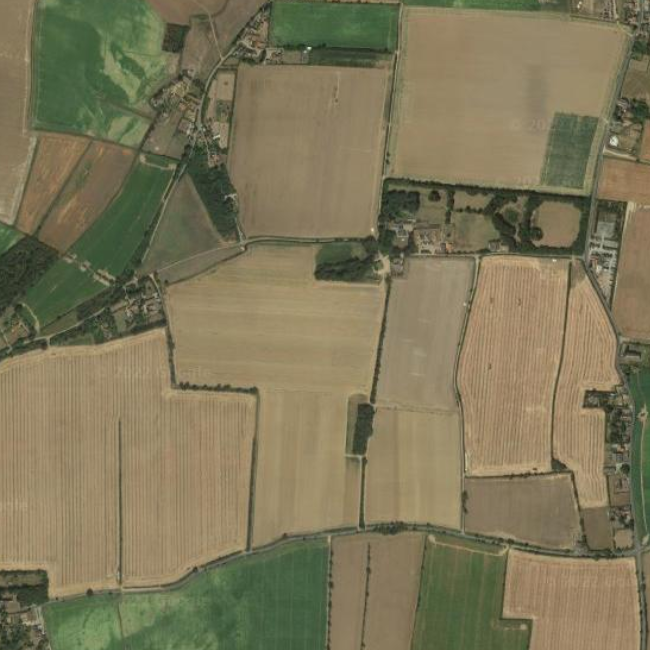
\includegraphics[width=6cm]{images/unlabeledMap.png}}}
            \qquad
            \subfloat[\centering Map with labels on roads]{{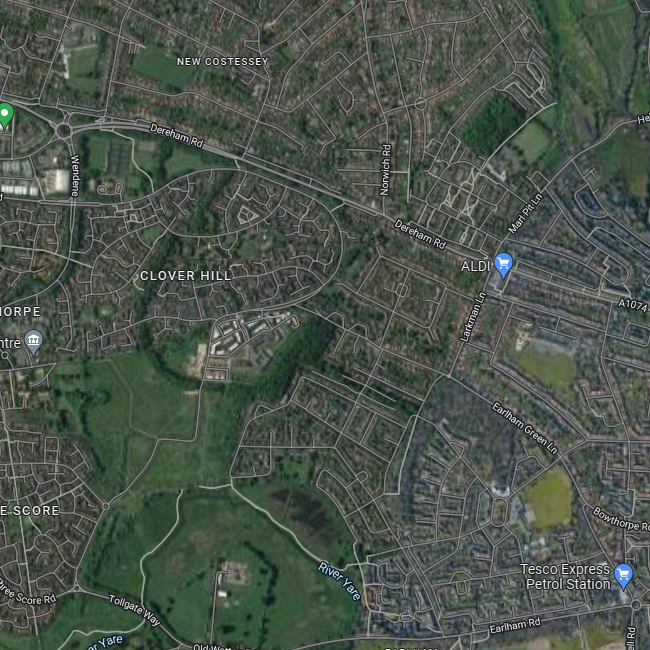
\includegraphics[width=6cm]{images/labeledMap.png}}}
            \caption*{Examples of maps with and without labels taken from Google Maps\textsuperscript{\textcopyright}}
        \end{figure}
        \bk

        This can cause issues for people who live out in areas which have not been mapped. This is because they cannot create easy to follow routes with the click of a button. Therefor, 
        causing people who live in rural areas to waste time getting used to the routes they have to take to go anywhere. Overall, the problem I am going to be creating a solution for is 
        how people are unable to easily go from point to point at the click of a button and be easily able to, at a glance, interpret the map without prior experience. \\

        \subsection{Background}
        \bk
        When people usually want to go about planning a journey they will use a service, for example Google Maps to get from one location to another. This usually takes the form of clicking 
        a location and then selecting an origin. This isn't always possible however, this can be for a multitude of reasons it seems however I will briefly go over some below:\\
        
        \begin{enumerate}
            \item \textbf{Either the destination or origin location(s) are not in the service's database.}
            \item \textbf{The destination and origin have no clear defined path between them.}
            \item \textbf{Either the destination or origin are off any predefined track.}
            \item \textbf{The travel method the user has selected is not able to traverse the terrain between the origin and destination.}
        \end{enumerate}

        \bk
        Some of these I believe are out of the scope of this project however once the interview has been conducted with the end user I will have a better idea of the needs that my program needs to for-fill.\\

        \bk
        Finally, I feel that the point of my final solution should be to fix all of the flaws which I find during my research as well as from the end user. As well as improving where the end user feels it needs to be. \\

        \bk
        
        \subsection{End User}
            \subsubsection{First Interview}
            \normalsize
            In order to get a better feel for the objectives and functions that my program should complete I interviewed with an end user, Mrs Mandy T. I believed that she was an appropriate candidate for this
            project due to the fact that she has to drive into work every morning. Along her route she has to deal with Google Maps which do not cover all of the roads in her area. Therefor in the following questions
            I asked her some questions gauge her priorities when it comes to web mapping.
            \bk
            \begin{enumerate}
                \item {\bf{When using web maps (e.g. Google Maps\textsuperscript{\tiny\textcopyright}) what are the key features you look for?}} \\
                \bk
                "A scale! WHY is it lost so often when Google Maps is embedded?! 
                Then it depends what type of map I'm looking at... if it's a road map then....roads! Size/type of road is important and things like one-way restrictions. 
                If it's for e.g. walking...footpaths/bridleways and parking are important. 
                "
                \item {\bf{Have you ever experienced a faulty or mislabeled part of an web map or has said map ever been inaccurate?}} \\
                \bk
                "Yes"
                \item {\bf{Do you often use web maps in your day to day life, if so in what capacity?}} \\
                \bk
                "Yes, \textbf{NEEDS TO BE ADDED TO}"
                \item {\bf{In your opinion do you feel that web maps are vital to every day life if so why or why not? }} \\
                \bk
                "No.  I passed my driving test before we had sat-nav or internet, so clearly they're not vital - we survived without them! \\ 
                They are quite helpful though as we used to have to buy a new road map every year, whereas web maps can be updated as things change, instead of only annually!"
                \item {\bf{What makes a good user interface for a web map?}} \\
                \bk 
                "Clarity and simplicity.  Nothing needlessly complicated."
                \item {\bf{How do you use web maps (e.g. long journeys, short journeys, school runs)?}} \\
                \bk
                "Route functionality on long or unfamiliar journeys. 
                Using them a lot at the moment as am planning a holiday overseas.  The maps are useful to see whether accommodation and restaurants will be walking distance, 
                and what options there are in each location etc."
                \item {\bf{Do you feel a tutorial would be beneficial to aid in the use of the map or should the focus more be spent on intuitive ease of use?}} \\
                \bk
                "If they're easy to use, a tutorial would be surplus to requirements, so ease of use is more important. "
                \item {\bf{Would it be beneficial to store old routes?}} \\
                \bk
                "Not really (is this a routing question?). I don't know what purpose that would give, unless I was being accused of something and needed to use the route as evidence of 
                being in a certain location! It could be use full in the context of frequently traveled routes however if this was the case I would know the route by heart anyway."
                \item {\bf{What forms of transport should the map include?}} \\
                \bk
                "(I think this is a routing question not a map question)
                Walking, bike/horse, car, bus, plane, ferry. 
                If just a map question, then the map should include footpaths, bridle paths, roads, ferry routes"
                \item {\bf{If there was one feature you could have implemented in an existing solution what would it be?}} \\
                \bk
                "To be able to post a question about a specific area and have a person who is local to that area answer it."
            \end{enumerate}
            
            \subsubsection{Evaluation of First Interview}
            Overall I feel that this interview gave me valuable insight into the requirements of my end user. As well as this my end user made it clear to me that there are two overriding 
            parts of this solution. The map recognition aspect of it and the path finding aspect. Going deeper into the path finding part of this project I will need to do research on the 
            different methods that will be used to achieve this and some of the possible data structures I could use. \\
        \bk

        \subsection{Initial Research} 
            \subsubsection{Existing Solutions}
            Below each overview passage I have included an image of each map for comparison of their GUI's. These will be used as inspiration as to how my final solution will look as well 
            as serving as examples of how the GUI can sometimes become overly complicated. This is especially the case with Bing Maps as when you initially access it you are flooded with 
            popups and extra options. \\
            \paragraph{Google Maps} \mbox{} \\
            \bk
            
            As aforementioned this is one of the most used forms of interactive web mapping in use at the moment. It has been in use since 8\textsuperscript{th} February 2005. As it exists
            now it is an interactive world map with routing features built in. It provides detailed information about geographical places and regions around the world. Unlike some of its
            competitors it also offers aerial and satellite images of places around the world aiding in navigation of terrain. \\
            
            \bk
            
            As well as its map viewing capabilities it also offers partial route planning and live route tracking for cars, bikes, walkers and public transport. It provides instantaneous and
            real time feedback while you are moving however the one big caveat to this is the fact that it will require an internet connection to run, something that is not always available. \\
            \bk
            
            \begin{figure}[H]
                \centering
                \subfloat[\centering Example of Google Maps' GUI]{{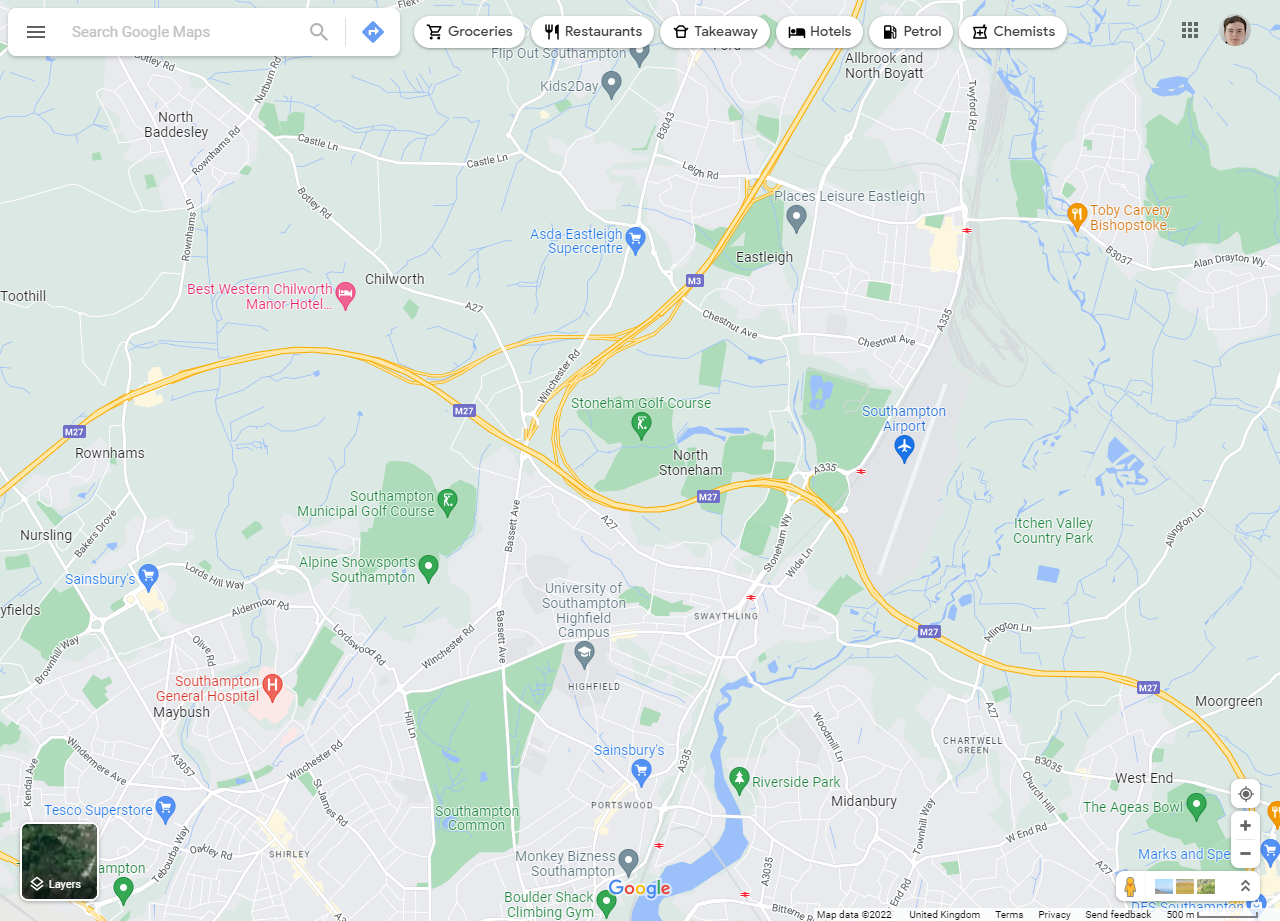
\includegraphics[width=7.5cm]{images/googleMapExample.png}}}
                \caption*{Sourced from Google Maps\textsuperscript{\tiny\textcopyright}}
            \end{figure}

            \bk 
            
            \paragraph{Bing Maps} \mbox{} \\
            This is another form of interactive web mapping. This is a more plain version of Google Maps at first glace. This is due to the fact that it does not have as many features as Google Maps.
            This does have its advantages due to the UI seeming less cluttered and more accessible. Similar to the Google Maps it also offers route planning and map traversal as well as live traffic updating.
            Bing maps unlike Google Maps boasts a more open API and easier programmatic interface for developers to be able to interface with their program. \\
 
            \bk
 
            Bing maps also still includes the feature which allows users to create their own maps based on their own data. Unlike google which did have this feature until they discontinued it.
            I believe that this could be something that would be beneficial to my program, allowing people to take a photo of their own map and have my solution compute it into a rotatable map. \\
 
            \bk
 
            \begin{figure}[H]
                \centering
                \subfloat[\centering Example of Bing Maps' GUI]{{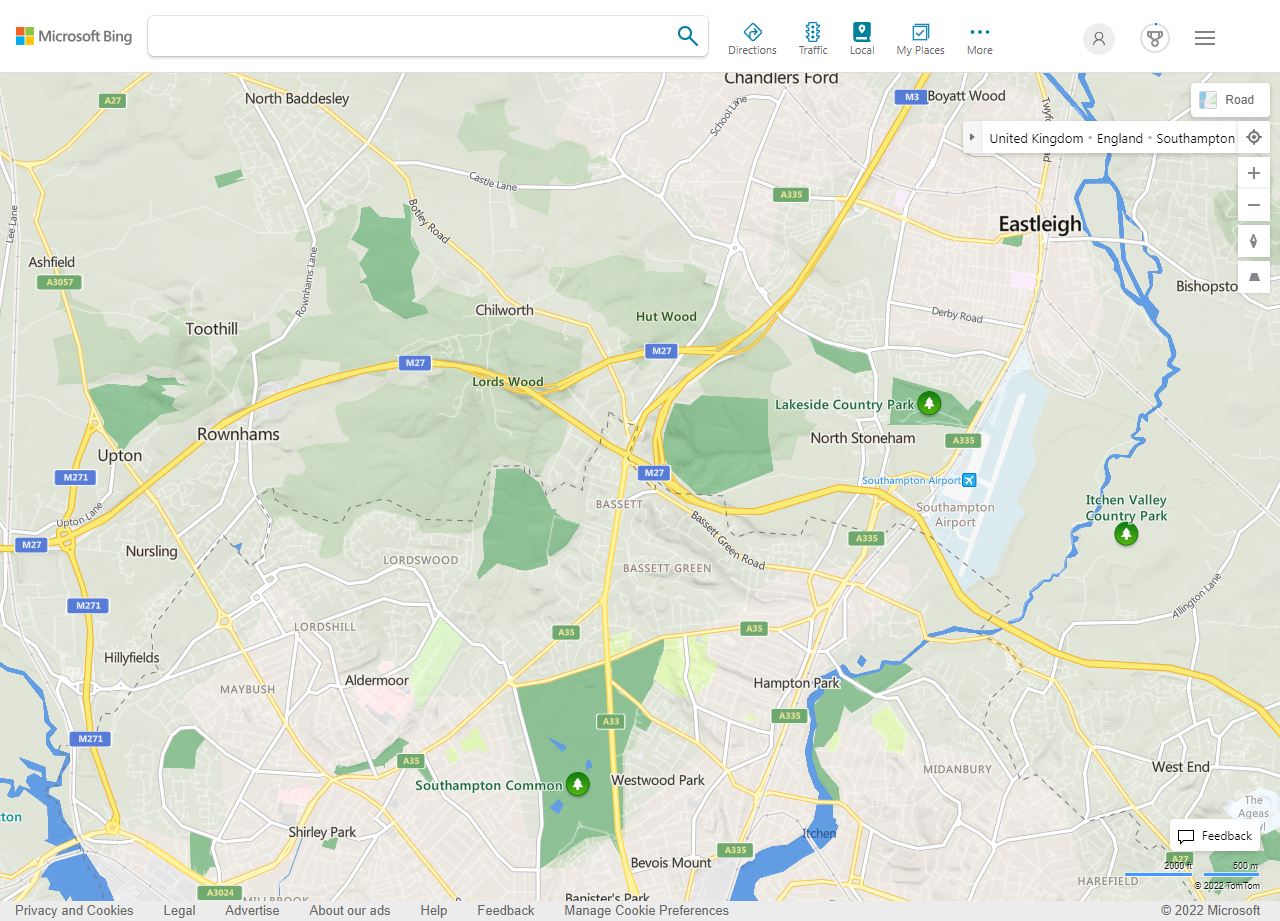
\includegraphics[width=7.5cm]{images/bingMapExample.png}}}
                \caption*{Sourced from Bing Maps\textsuperscript{\tiny\textcopyright}}
            \end{figure}

            \bk

            \paragraph{OS Maps} \mbox{} \\
            This is a different take in web mapping compared to Bing and Google Maps. With Ordnance Survey their focus was on the accuracy of their maps hence they do not have as an extensive routing system.
            If you wanted to go from point to point on an OS map you would have to plot it by hand. However if you wanted to go on an exercise trail on the other hand they are very well suited
            for this and as such have an extensive list of pre-planned routes. \\
            \bk
            Similar to Google Maps, and in a limited capacity, Bing maps; OS Maps allow you to view their maps in different forms such as 3D and topographic however in order to access these you will
            have to access their premium plan therefore for the average user this is not a viable option and a hindrance. It is good to note however that the other variations on the map of the UK,
            and this holds true for all of the aforementioned maps, that the satellite view and other views are not necessary and could in fact be a hindrance. \\
            
            \bk
            
            \begin{figure}[H]
                \centering
                \subfloat[\centering Example of Ordnance Survey's Map GUI]{{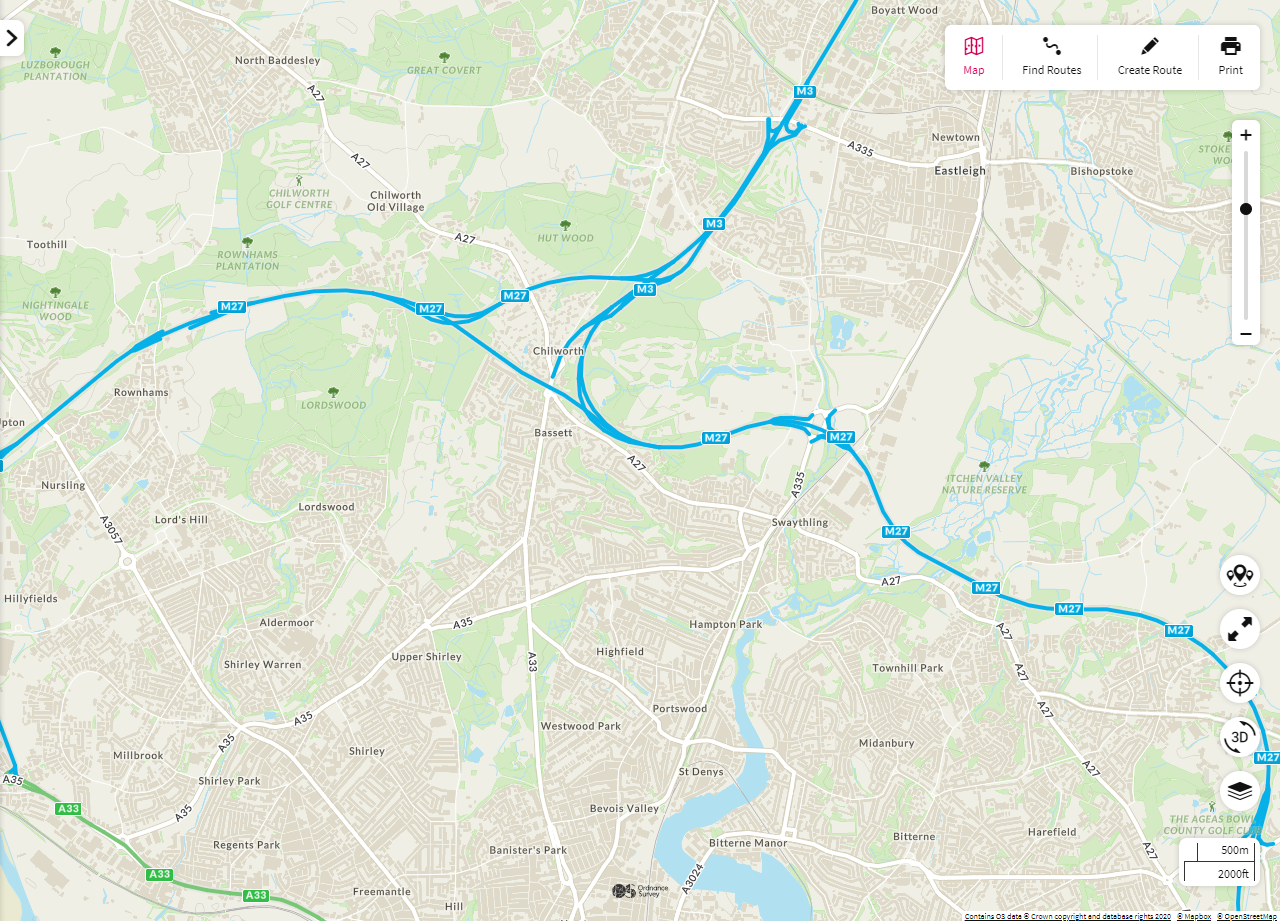
\includegraphics[width=7.5cm]{images/osMapExample.png}}}
                \caption*{Sourced from OSMaps.com\textsuperscript{\tiny\textcopyright}}
            \end{figure}

            \bk
            
            \paragraph{Existing Solutions Conclusion} \mbox{} \\
            In conclusion, I have found that the existing solutions that are available are all very well designed and well implemented. I have found that they are easy to use and rather intuitive
            however, for the average user who just needs to get from A to B in the most economic way possible they are overly complicated. As well as this I have found that with the exception of OS maps
            both of the other solutions require an internet connection to get the best use out of their maps, this is something which I believe I should avoid. This will mean that all calculations will 
            have to occur self contained within the program, not allowing the use of external API's. \\
            \bk

            \subsubsection{Possible Algorithmic Solutions}
            There are, as aforementioned many existing solutions which work in various ways, in order to make my solution unique and functioning I am going to have to incorporate many different algorithms
            and theories. \\ \bk

            \paragraph{Edge Detection} \mbox{} \\
            First of all I will need some way of recognising a map and parsing it in some way. The way that first springs to mind is edge detection. This is a way of taking an image and computing where there
            are changes in contrast or brightness which could be considered an edge. There are many forms of edge detection out there all of which work in various ways, the main things they look for however
            are discontinuities in depth, discontinuities in surface orientation, changes in material properties and variations in scene illumination. All of these factors combine and allow a program to decide
            if there is an edge in an image. \\ \bk

            A simple edge detection model can be extremely effected by natural blur or artifacts in an image. In order to mitigate this there are smoothing algorithms that can be used to blur and smooth edges
            causing the impact of artifacts to be avoided. The common term when referring to artifacts and erroneous data in an image is \emph{noise}. I believe it will be beneficial to include some of these
            in my solution, this will be something to look into in the \textbf{Further Research} section. \\ \bk

            Taking a quick look at one form of edge detection, Canny Edge detection, it is relatively simple in its implementation. It has only 5 steps, first removing noise with a Gaussian filter then applying
            bounding to the image and finally performing hysteresis threshold. This is the most common form of edge detection that I have come across in my research however there are others. A rather
            different example of edge detection is Kovalevsky edge detection. Unlike canny edge detection this does not care about the luminosity of the image and goes based of the colour intensity in each
            of the channels. \\ \bk

            \paragraph{Graph Forming} \mbox{} \\
            This is not so much a possible algorithmic solution but more of something that my solution will have to achieve. Once the image of the map has been altered and the edge detection has been 
            performed, I will be left with an image which has white lines where there "edges". From this I will need to create a weighted graph as well as an unweighted graph. \\ \bk
            
            During my research I have failed to come across an existing solution to this problem. As well as this looking through some examples that people have uploaded it seems that sometimes the edge 
            detection does not yield a fully connected image. This could prove to be an issue as it would add the possibility of isolating certain roads. \\ \bk
            
            I feel that I need to look more into this and come up with my own solution during the prototyping stage, and come up with my own algorithmic way of generating it. \\ \bk
            
            \bk

            \subsubsection{Key Components Required}
            After doing my initial research and a brief look at the existing solutions I have come up with, what I feel, is the main 4 Components that I will need to build my solution. \\ \bk
            
            \paragraph{The Graphical User Interface} \mbox{} \\
            Talking to my end user made it clear to me that in order for the program to be usable by the wider population it would need to be clean and uncluttered. This leaves me in a difficult position 
            due to there being a limited amount of frameworks that are available to me. I have two sets of possibilities: \\
            \begin{enumerate}
                \item A Local App Run on Device
                \item A Web Based Application
            \end{enumerate}
            Each of these have their advantages, if I where to go with a locally run app I could make it in the console keeping it simplistic and easy to use. However if I do use the console it would limit
             this solution to a computer which could be seen as going against the idea of this problem. On the other hand, if I where to go with a web server based application this would yield much better 
             compatibility with all devices since all you would need is access to a web browser. This, by its very nature, means that you would need an internet connection which is also a problem which I
              was hoping to fix. \\ \bk
            
            The solution then I believe is to make it both a locally based program with the option for it to run a web server. However I will need to specify one over the other to begin with to make sure
             that the program is working either way. \\ \bk
            
            Regardless of which one I choose I will conduct some form of testing where I will allow, through a survey, people to specify what makes an easy to use and intuitive. \\ \bk
            
            \paragraph{Image Manipulation and Edge Detection} \mbox{} \\
            This is perhaps the most important part of the project since without this I would not be able to continue to path find the image of the map. Looking at my research I feel that there will be a combination of 
            \bk
            
            \paragraph{Graph Creation and Representation} \mbox{} \\
            From lessons which we have had in class I have been shown that there are 2 reasonable ways of representing a graph in code, this includes an adjacency matrix and an adjacency list. Both have their advantages and disadvantages. An adjacency matrix is good when you have a reasonably connected graph which has weights, this is due to it being easy to access and traverse. As soon as you have a sparse graph however it becomes very memory intensive which is unnecessary considering that there will be very few of the cells with actual data in them. This is when the adjacency list comes into play, the reason that I am reluctant to use this form of representing a graph is that when performing some of the various graph traversal algorithms it can incredibly difficult and pointless to adapt them when by adapting them you effectively generate the adjacency matrix.
            \bk
            
            \paragraph{Graph Traversal and Output} \mbox{} \\
            \bk


        \subsection{Further Research}
            \subsubsection{Dive into Specific Algorithms}
            After doing some research it seems that there needs to be a set of definitions before I go any further to avoid confusion. This is because during my time on Wikipedia there are sections
            where several terms are used interchangeable where I feel they are not the same. Each of these definitions are as defined by me and are not necessarily the official definitions since they 
            do not explicitly exist. They are as follows: \\ \bk
            \begin{enumerate}
                \item Graph Traversal: The act of routing or searching through a graph from one node to another, either using an algorithm or by another means.
                \item Graph Routing: Graph traversal in a \emph{weighted undirected} graph.
                \item Graph Searching: Graph traversal in a \emph{unweighted undirected} graph.
            \end{enumerate}

            \bk
            The difference is slight however the key takeaway from this is that when I am referring to a Routing algorithm I am referring to one which works on a weighted graph. And vice versa if I am 
            talking about a searching algorithm this is referring to graph traversal on an unweighted graph. \\ \bk

            \paragraph{Black and White Filter}\mbox{} \\
            In order to allow the program to function, assuming that the canny edge detection was chosen we do not need the colour data of the image. In order to remove this a filter is used, this one is the
            industry standard since it takes into account how prevalent red, green and blue are rather than taking an average which could become non representing of the real case. \\ \bk
            
            \begin{gather*}
                \beta = 0.299 * \alpha_{b} + 0.587 * \alpha_{g} + 0.114 * \alpha_{b}
                \text{; }
                \begin{cases}
                    255 & \beta > 255 \\
                    0 & \beta < 0 \\
                    \beta & \beta \in [0, 255]
                \end{cases}
            \end{gather*}
            
            \BK

            If an averaging was used it would just be, this is also known colloquially as the "quick and dirty" method. \\ \bk
            \begin{gather*}
                    \beta = \frac {(\alpha_{b} + \alpha_{g} + \alpha_{b})}{3}
            \end{gather*}

            \bk
            \paragraph{Gaussian Filter} \mbox{} \\
            This is the first step of 5 in terms of performing Canny Edge Detection. Applying the Gaussian filter to the image will smooth out the image and remove any noise. It does this by taking a section
            of the image, sometimes referred to as a kernel and performing an equation on it. Once it has computed the equation it sets all of the pixels inside the kernel to this value. The following is true 
            for a kernel size of $(2k + 1) * (2k + 1)$. It takes two changeable parameters $\sigma$ which denotes the amount of blur to apply and $k$ is the kernel size. As well as being one of the key steps in canny edge detection it is also a vital component to most edge detection programs since noise can cause errors in the final image.\\ \bk
            
            \begin{gather*}
                H_{ij} = \frac{1}{
                    2\pi\sigma^{2}
                } \exp \bigg(
                    -\frac{
                        (i - (k + 1))^{2} + (j - (k + 1))^{2}
                    }
                    {
                        2\sigma^{2}
                    }
                \bigg);1\leq i, j \leq(2k+1)
            \end{gather*}

            \BK
            Since the Gaussian kernel I would be using would always be centred around the origin $(0, 0)$ I can use a simplified version of the Gaussian distribution equation. This is as follows: \\ \bk
            
            \begin{gather*}
                H_{ij} = \frac{1}{2\pi\sigma^2} \exp \frac{-(x^2 + y^2)}{\sigma^2}
            \end{gather*}
            
            \BK
            I can afford to remove the $(i - (k + 1))$ section due to the fact that I am not having to calculate the Gaussian distribution at a non-centred location. One notable thing to mention is that in many cases it is not necessary to calculate the Gaussian kernel by hand and an approximation can be used. The example below is the approximation when $\sigma$ has a value of 1. \\ \bk
            
            \begin{gather*}
                B = \frac{1}{159} \begin{bmatrix} 
                2 & 4 & 5 & 4 & 2\\
                4 & 9 & 12 & 9 & 4\\
                5 & 12 & 15 & 12 & 5\\
                4 & 9 & 12 & 9 & 4\\
                2 & 4 & 5 & 4 & 2
                \end{bmatrix} * A
            \end{gather*}
            \bk
            
            \paragraph{Convolution Operation} \mbox{} \\
            Convolution is the method at which most image manipulation is achieved. It evolves taking a altering kernel and a kernel of the original image and then combines the two through convolution. The generalised equation for this is as follows. \\ \bk
            
            \begin{gather*}
            {\displaystyle {\begin{bmatrix}x_{11}&x_{12}&\cdots &x_{1n}\\x_{21}&x_{22}&\cdots &x_{2n}\\\vdots &\vdots &\ddots &\vdots \\x_{m1}&x_{m2}&\cdots &x_{mn}\\\end{bmatrix}}*{\begin{bmatrix}y_{11}&y_{12}&\cdots &y_{1n}\\y_{21}&y_{22}&\cdots &y_{2n}\\\vdots &\vdots &\ddots &\vdots \\y_{m1}&y_{m2}&\cdots &y_{mn}\\\end{bmatrix}}=\sum _{i=0}^{m-1}\sum _{j=0}^{n-1}x_{(m-i)(n-j)}y_{(1+i)(1+j)}}
            \end{gather*} \bk

            To give a more comprehensive example this can be simplified down to:

            \begin{gather*}
                \displaystyle \left({\begin{bmatrix}a&b&c\\d&e&f\\g&h&i\end{bmatrix}}*{\begin{bmatrix}1&2&3\\4&5&6\\7&8&9\end{bmatrix}}\right)\\  \\
                \rightarrow{} (i\cdot 1)+(h\cdot 2)+(g\cdot 3)+(f\cdot 4)+(e\cdot 5)+(d\cdot 6)+(c\cdot 7)+(b\cdot 8)+(a\cdot 9)
            \end{gather*}

            \bk
            The simplest way of thinking of this is that you are performing matrix multiplication on a two matrices except one of them has been flipped both vertically and horizontally. Mapping the point [2, 2] to [0, 0].

            \subsubsection{Second Interview}
            \normalsize
            Now that I have done some more research into the various ways there are to complete this task I have formed some more questions to ask my end user to get a solid and
            defined list of objectives for the program. AI will couple this with my research to form a complete plan to form said objectives. As well as this however the second interview
            will allow me to correct any inaccurate questions that where asked in the initial interview. This is because after I received my initial responses I realised that I
            needed to be more clear with what I was asking and the information that I wanted back. \\
            \bk

            HAS BEEN ASKED WAITING FOR RESPONSES
            \begin{enumerate}
                \item {\bf{Bobbert?}} \\
                \bk
                bobbert.
                \item {\bf{Cobbert?}} \\
                \bk
                cobbert.
                \item {\bf{Dobbert?}} \\
                \bk
                dobbert.
                \item {\bf{Fobbert?}} \\
                \bk
                Fobbert.
                \item {\bf{Norbert?}} \\
                \bk
                norbert
                \item {\bf{Dilbert?}} \\
                \bk
                dilbert.
                \item {\bf{Bobbert?}} \\
                \bk
                bobbert.
            \end{enumerate}

            \subsubsection{Evaluation of Second Interview}
            After conducting this second interview I feel I now have a firm understanding of what I need to achieve with this program. I will also take this opportunity to create a prototype of the 
            the different parts of the program to gauge the difficulty of the program and any problems I may encounter before moving onto the final solution. \\ \bk
            Apart from that however I feel the interview went\dots % add to this

        \subsection{Prototyping}
        \subsubsection{Prototype Objectives} 
        Before I begin the creation of my prototypes I will create a list of sections I wish to complete by the end. This will allow me to keep perspective and make sure that the prototype remains on track. I have decided that the parts of my final solution are:
        
        \begin{itemize}
            \item A version of edge detection
            \item A graph class with basic traversal
            \item A forms interface for showing images
        \end{itemize} \bk
        

        \subsubsection{Edge Detection}
        For the example of edge detection which I am going to prototype I have chosen Canny Edge Detection, this is the most common of the types of edge detection and is relatively simple. It is also widely documented which allows me to focus more on the application and less on the finding of resources. \\ \bk

        Before I begin, there are a couple of key features that need to be mentioned. The first is how I handle building the image kernel. For example when the center pixel is on the edge of the image, you will have some non existent pixels as part of the image kernel. To combat this there are several methods:
        
        \begin{enumerate}
            \item Extension - The nearest border pixels to the chosen pixel are extended in order to fill the gaps. The corner pixels are extended at 90 deg. Others are extended in straight lines.
            \item Wrapping - The pixels for the unknown ones are taken from the opposite side of the image. For example it it was 1 off the top the first pixel from the bottom would be used.
            \item Mirroring - The image is mirrored at the edges doubling up the total image.
            \item Constants - Any pixels in the kernel which are not contained in the image are given a default value, this is usually grey or black depending on the application.
            \item Duplication - Similar to above any pixels which are not contained are set to the value of the center pixel in the kernel.
        \end{enumerate} \bk
        
        \begin{figure}[H]
            \centering
            \subfloat[\centering Wrapping]{{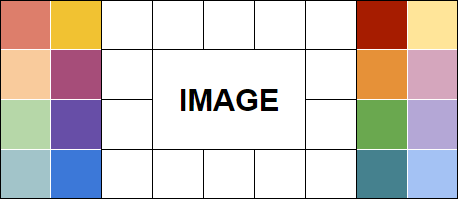
\includegraphics[width=4.5cm]{images/kernelExamples/wrap.png}}}
            \qquad
            \subfloat[\centering Mirroring]{{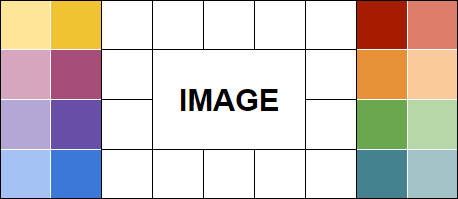
\includegraphics[width=4.5cm]{images/kernelExamples/mirror.png}}}
            \\ \BK
            \qquad
            \subfloat[\centering Extension]{{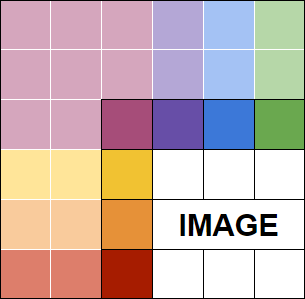
\includegraphics[width=2.5cm]{images/kernelExamples/extend.png}}} \space
            \qquad
            \subfloat[\centering Constants]{{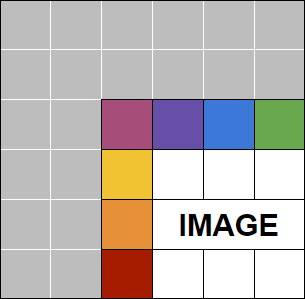
\includegraphics[width=2.5cm]{images/kernelExamples/constant.png}}}
            \qquad
            \subfloat[\centering Duplication]{{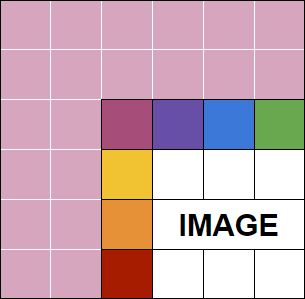
\includegraphics[width=2.5cm]{images/kernelExamples/clone.png}}}
        \end{figure}
        

        For this part of the prototype I have decide to go with the duplication option, this is due to the fact that it is one of the easier and quicker methods to implement as well as being suitable for the edge detection use case. \\ \bk
        
        \begin{figure}[H]
            \centering
            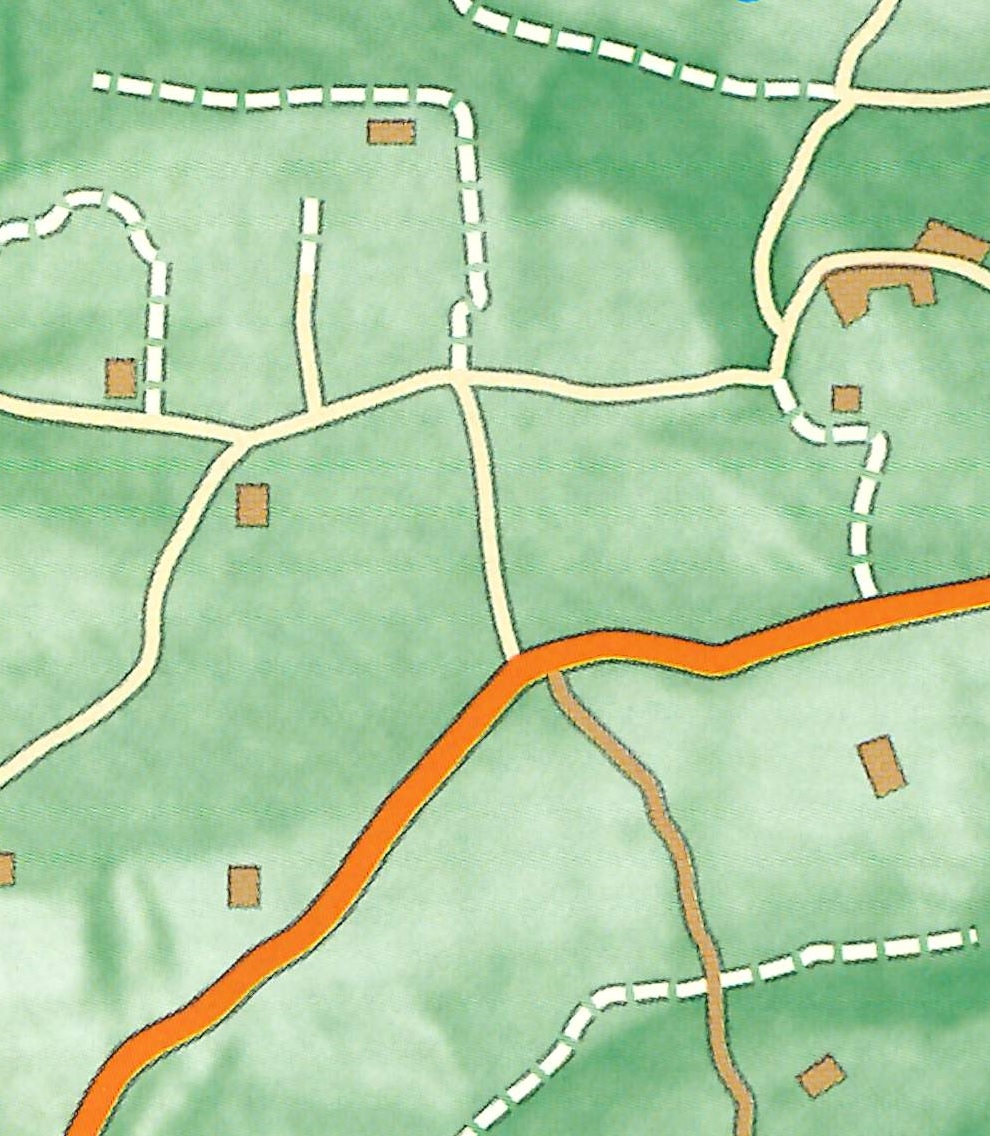
\includegraphics[width=5cm]{images/edgeDetectionPrototype/in.jpg}
            \caption{Original Image}
            \label{fig:proto_original}
        \end{figure}
        
        \paragraph{1. Converting to Black and White} \mbox{} \\
        The first part of the edge detection is to convert the image to black and white. This is because if the image is in colour then you would have to either perform edge detection on each of the colour sections and then somehow combine them, or take a single colour value to base the conversion off of. As previously mentioned this can be accomplished through many means, the most common as explained in \textit{1.5.1 Black and White Filter}. The version which I have decided to use for this prototype is the industry standard Y\textsuperscript{'}UV conversion. \\ \bk
        
        The implementation in code of this is as below:
        \begin{cscode}
public double[,] BWFilter(Bitmap image)
{
    double[,] result = new double[image.Height, image.Width];

    for (int i = 0; i < image.Height; i++)
    {
        for (int j = 0; j < image.Width; j++)
        {
            Color c = image.GetPixel(j, i);
            double value = c.R * 0.299 + c.G * 0.587 + c.B * 0.114;

            result[i, j] = Bound(0, 255, value);
        }
    }

    return result;
}
        \end{cscode}
        
        This takes the original image in Bitmap form and then instantiates an array with the dimensions of the input image, this will serve going forward as the array as to which all changes will be based from. I learnt from this prototype early on that when calculating the values is is better to use the exact ones from the previous stage. This is because if all the values where compressed to within image specifications ($0 \leq x \leq 25$) you would loose definition and precision causing later calculation so be incorrect. Once this section has run through every pixel in the image and converted it to a black and white value the subroutine returns the double array with the black and white values. The result of this on the input \textit{figure \ref{fig:proto_original}} is: \\ \bk
        
        \begin{figure}[H]
            \centering
            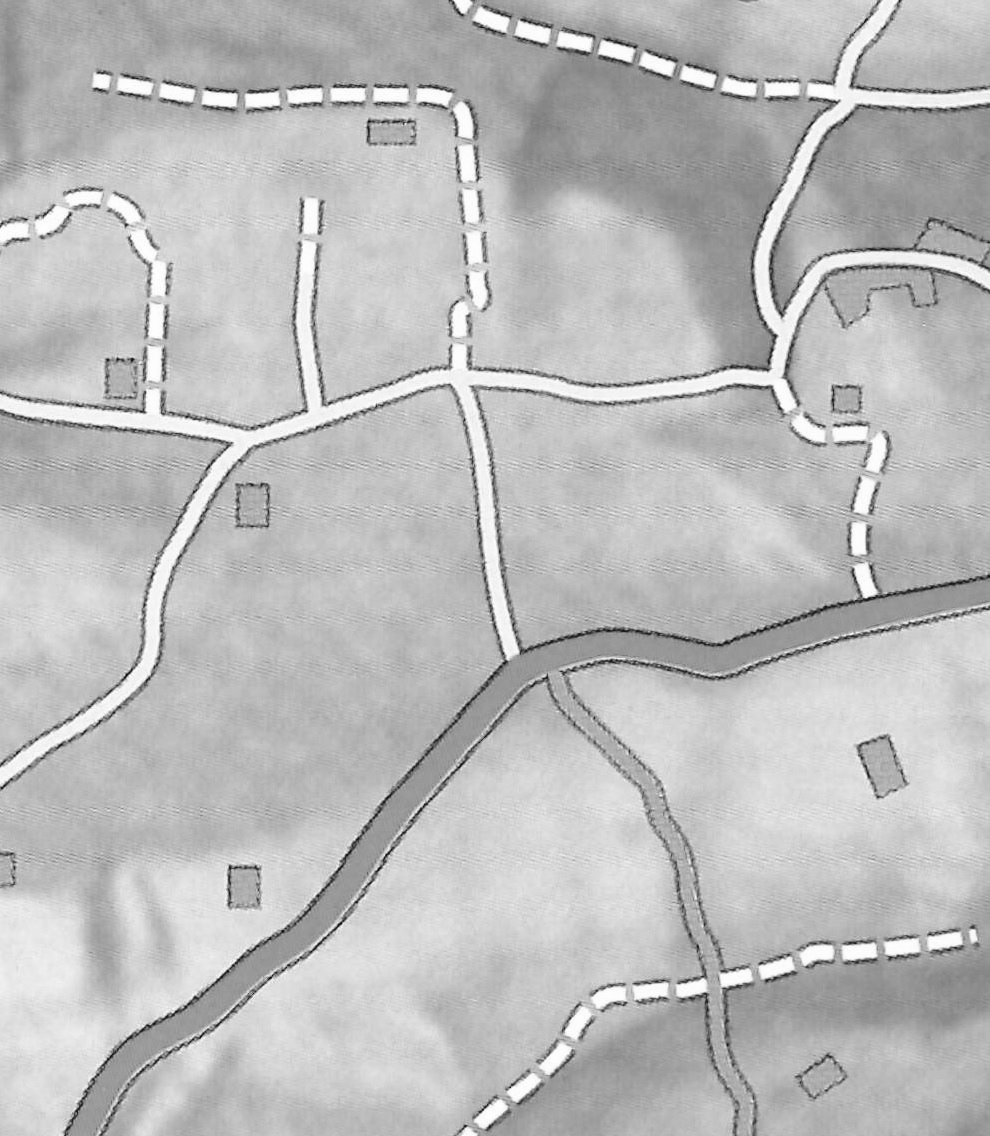
\includegraphics[width=5cm]{images/edgeDetectionPrototype/a.jpg}
            \caption{Black and White Filter}
            \label{fig:proto_bwfilter}
        \end{figure} \bk
        
        \paragraph{2. Gaussian Filter} \mbox{} \\
        The next step of canny edge detection is applying the Gaussian filter. This is to ensure that any noise that is contained within the image is removed. This is because if there are stray pixels in the center of the image this can cause an edge to form when in fact there isn't one. This is the first operation in edge detection which requires convolution as explained in \textit{1.5.1 Gaussian Filter}. To accomplish this the following code was used: \\ \bk
        
        \begin{cscode}
public double[,] GaussianFilter(double sigma, int kernelSize, double[,] imageArray)
{
    double[,] result = new double[imageArray.GetLength(0), imageArray.GetLength(1)];

    Matrix gaussianKernel = GetGaussianKernel(kernelSize, sigma);

    for (int i = 0; i < result.GetLength(0); i++)
    {
        for (int j = 0; j < result.GetLength(1); j++)
        {
            Matrix imageKernel = BuildKernel(j, i, kernelSize, imageArray);
            double sum = Matrix.Convolution(imageKernel, gaussianKernel);
            result[i, j] = sum;
        }
    }

    return result;
}
        
public Matrix GetGaussianKernel(int k, double sigma)
{
    double[,] result = new double[k, k];
    int halfK = k / 2;

    double sum = 0;

    int cntY = -halfK;
    for (int i = 0; i < k; i++)
    {
        int cntX = -halfK;
        for (int j = 0; j < k; j++)
        {
            result[halfK + cntY, halfK + cntX] = GetGaussianDistribution(cntX, cntY, sigma);
            sum += result[halfK + cntY, halfK + cntX];
            cntX++;
        }
        cntY++;
    }

    for (int i = 0; i < k; i++) for (int j = 0; j < k; j++) result[i, j] /= sum;
    return new Matrix(result);
}
        \end{cscode}
        
        Again this subroutine follows a similar layout to the rest in this prototype, it iterates though each pixel in the image and apply some equation. In this case as stated above it is performing convolution of a matrix which is a sub section of the original image. It is convoluting this with the Gaussian kernel though the means described in \textit{1.5.1 Convolution Operation}. The code for the convolution operation can be seen at \textit{5.1.1 Lines 586 through 612} and the Gaussian distribution lambda function can be found \textit{5.1.1 Line 554}. Another learning experience here was how if the image is sufficiently large then the kernel does not have as much of an effect at blurring the image and removing noise. It may be beneficial in the final program to reduce the image to a smaller size or perhaps change the sigma and kernel size. The output of this subroutine is: \\ \bk

        \begin{figure}[H]
            \centering
            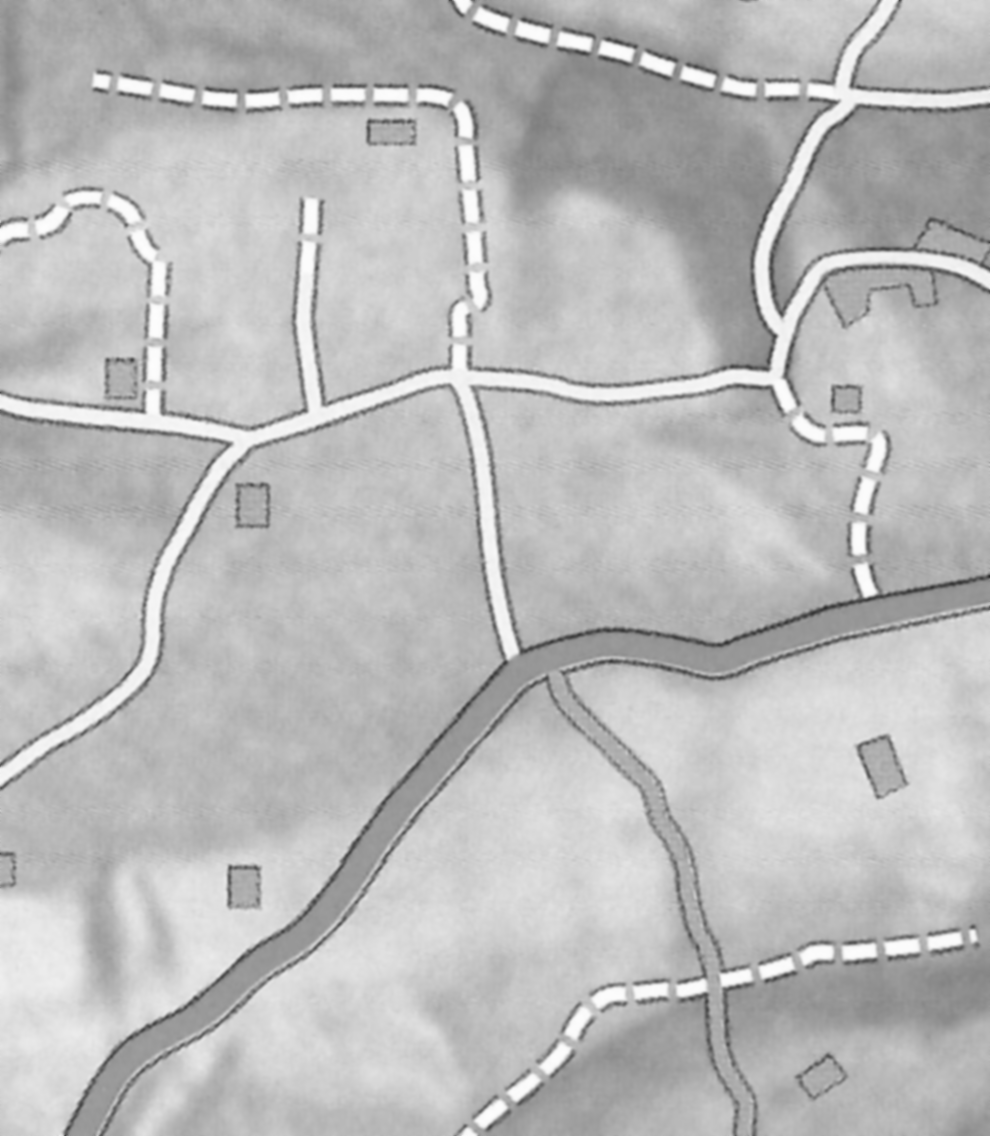
\includegraphics[width=5cm]{images/edgeDetectionPrototype/b.jpg}
            \caption{Gaussian Filter}
            \label{fig:proto_guaussian}
        \end{figure} \bk
        
        \paragraph{3. Calculation of XY Gradients} \mbox{} \\
        The first edge picking stage of canny edge detection is the calculation of the gradients of the image in both the X axis and the Y axis. In order to achieve this two more kernels are used. They are known as the Sobel operators. \\
        \begin{gather*}
            {\displaystyle M_{y}={\begin{bmatrix}+1&0&-1\\+2&0&-2\\+1&0&-1\end{bmatrix}}\quad {\text{and}}\quad M_{x}={\begin{bmatrix}+1&+2&+1\\0&0&0\\-1&-2&-1\end{bmatrix}}}
        \end{gather*} \bk
        
        The code which is used to perform this section of the canny edge detection is as follows, note that for the gradient in Y the matrix is replaced with the Y matrix and its code can be seen at \textit{5.1.1 Lines 416 through 432}. \\ \bk
        
        \begin{cscode}
public double[,] CalculateGradientX(double[,] imageArray)
{
    double[,] result = new double[imageArray.GetLength(0), imageArray.GetLength(1)];

    Matrix sobelX = new Matrix(new double[,] {
        { 1, 2, 1 },
        { 0, 0, 0 },
        { -1, -2, -1 },
    });

    for (int i = 0; i < imageArray.GetLength(0); i++)
    {
        for (int j = 0; j < imageArray.GetLength(1); j++)
        {
            Matrix imageKernel = BuildKernel(j, i, 3, imageArray);
            result[i, j] = Matrix.Convolution(imageKernel, sobelX);
        }
    }

    return result;
}
        \end{cscode}
        
        Same as the Gaussian filter the convolution operation is applied to both of these matrices. The kernels that are used are build from the image with the center $(i,j)$ same as the previous step. This is when it becomes beneficial to use the duplication method for the kernel building. Since the gradient is dependent on the surrounding pixels using the pixel itself prevents false edges from appearing. The two separate gradient kernels produce the following images:
        
        \begin{figure}[H]
            \centering
            \subfloat[Gradient in X]{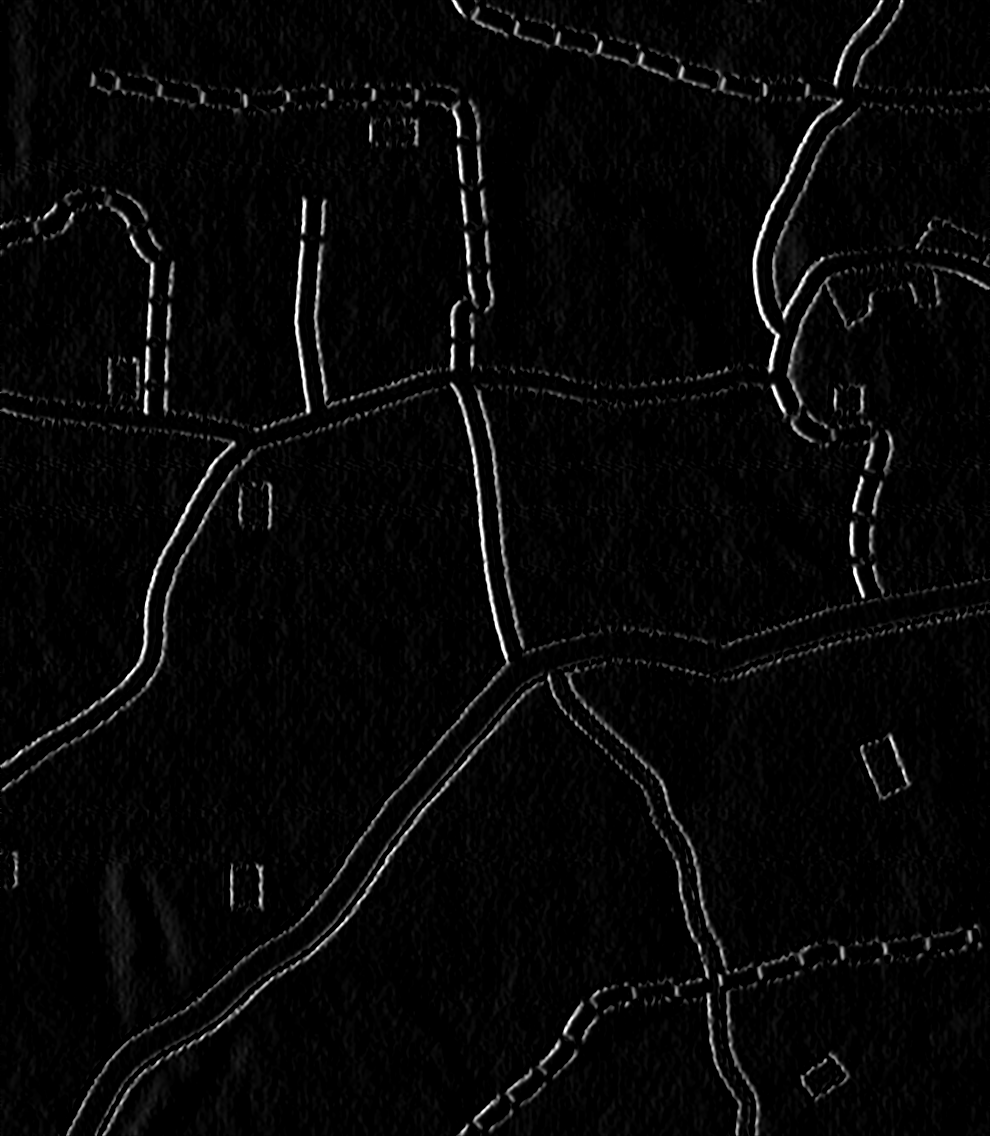
\includegraphics[width=5cm]{images/edgeDetectionPrototype/c.jpg}}
            \label{fig:proto_gradX}
            \qquad
            \subfloat[Gradient in Y]{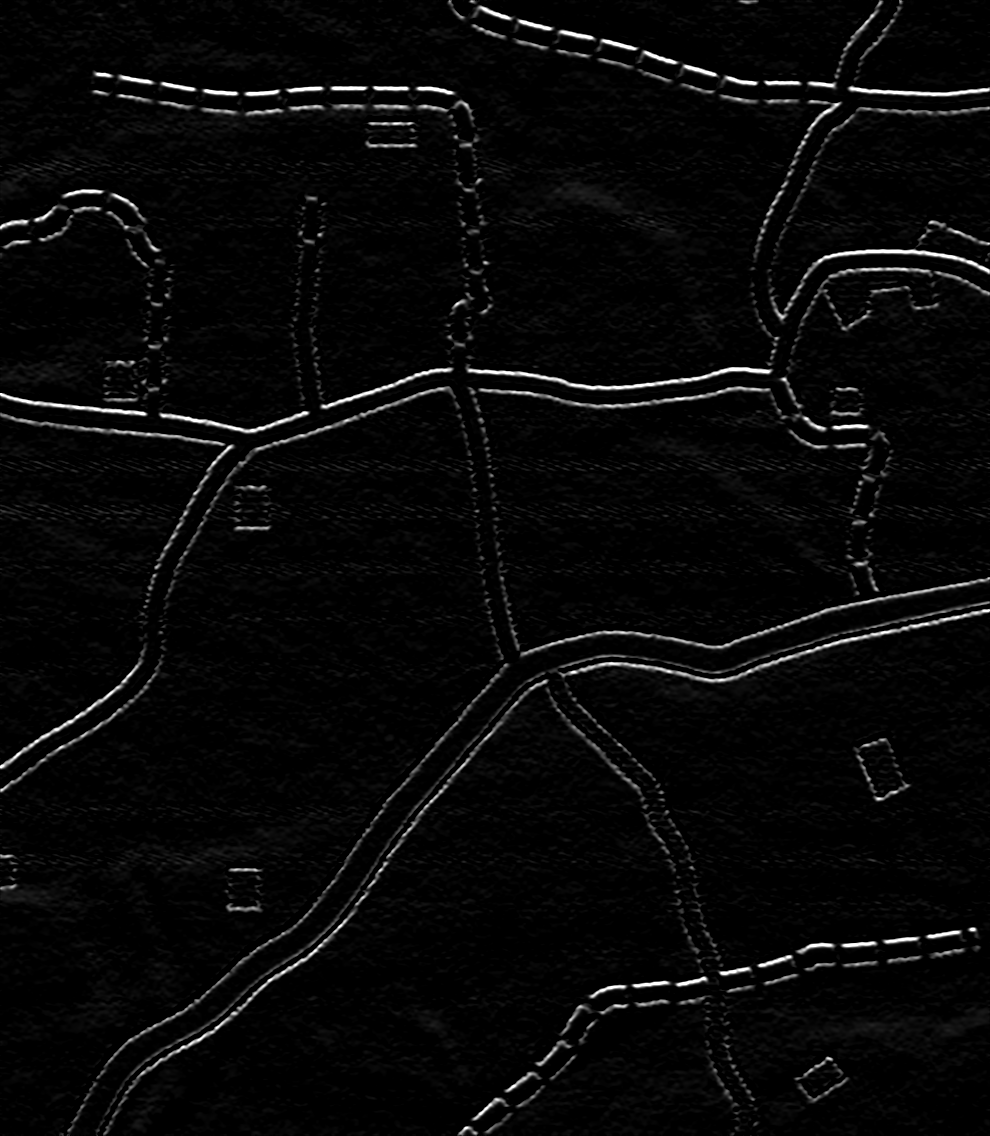
\includegraphics[width=5cm]{images/edgeDetectionPrototype/d.jpg}}
            \label{fig:proto_gradY}
        \end{figure} \bk
        
        These two images represent the cases where in the image there is a change in the value of the pixels. The brighter the white the more different two given pixels are. We can combine these two to give a total image of all gradient changes. Find image below, while this is useful to look at from a human perspective it is not the most useful in edge detection and in fact we will need both the raw 2D double arrays from each gradient calculation to move onto the next step.
        
        \begin{figure}[H]
            \centering
            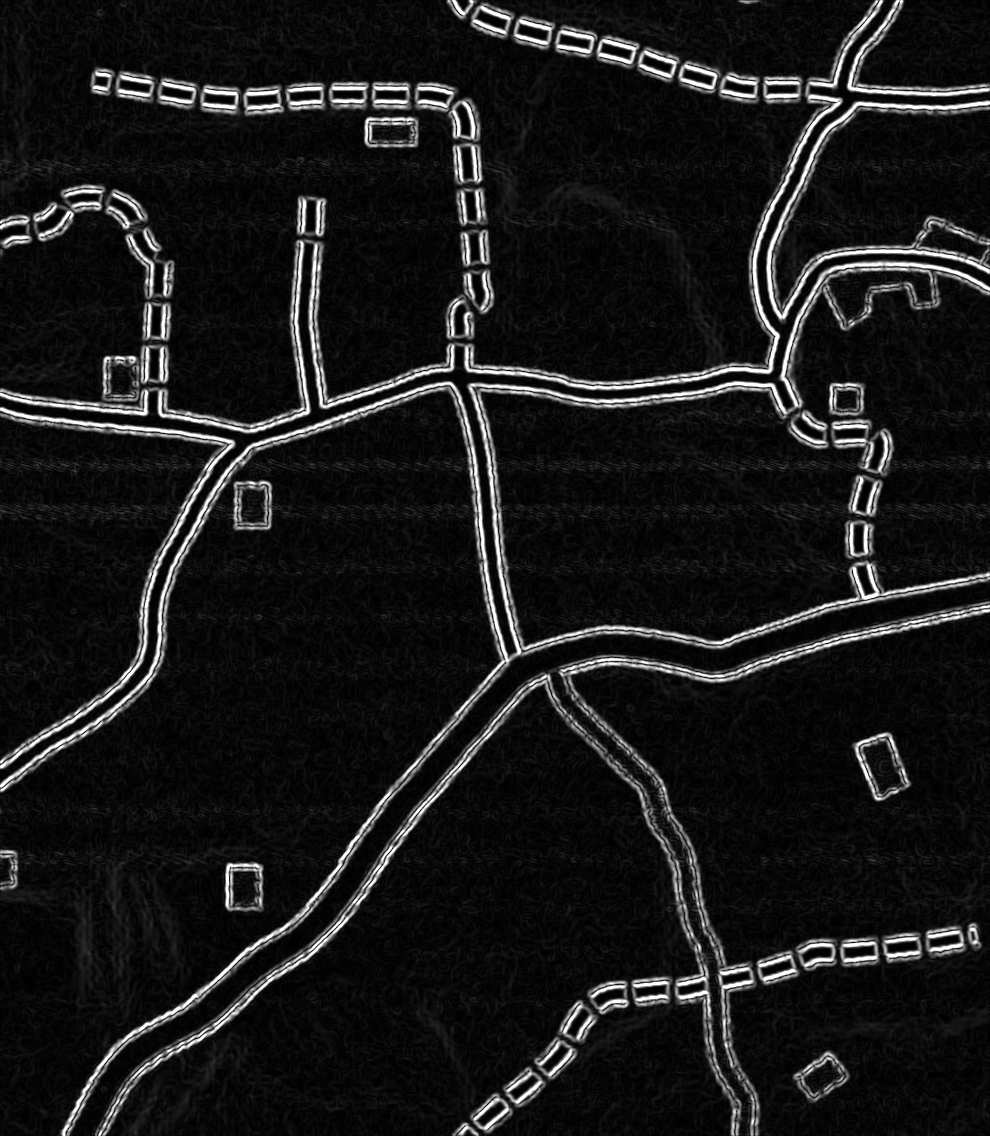
\includegraphics[width=5cm]{images/edgeDetectionPrototype/e.jpg}
            \caption{Gaussian Filter}
            \label{fig:proto_gradTot}
        \end{figure} \bk
        
        \paragraph{4. Gradient Direction} \mbox{} \\
        Now that the gradient values have been calculated we can move onto working out which direction the gradient is travelling. This is done via the use of the $2^{nd}$ argument arc-tangent. The definition of the $2^{nd}$ argument arc-tangent is defined as the angle in the Euclidean plane, given in radians, between the positive $x$ axis and the ray from the origin to the point $(x,y)$. Once this is calculated this will allow the program to see in which direction the gradient is travelling in the image. As well as this is also allows us to see how sharp the change is from one to the other, this is how we can decide if there is an edge there. The code to calculate the $2^{nd}$ argument arc-tangent is simple since all is needed is to iterate over the entire image. The code for this can be seen at \textit{5.1.1 Lines 379 through 384.}
        
        \begin{cscode} 
public double[,] CalculateTheta(double[,] gradX, double[,] gradY)
{
    double[,] result = new double[gradX.GetLength(0), gradX.GetLength(1)];
    for (int i = 0; i < gradX.GetLength(0); i++) for (int j = 0; j < gradX.GetLength(1); j++) result[i, j] = Math.Atan2(gradY[i, j], gradX[i, j]);
    return result;
}
        \end{cscode}
        
        This however will return an array with values which are in the range of -$\pi$ to $\pi$ therefore in order to create an image to visualise the result a linear transformation must be used which can be calculated as the equation of a line. The derived equation is $\frac{128}{2\pi}x + 128$ where x is the value of theta. Once converted the output of this stage is as follows.
        \begin{figure}[H]
            \centering
            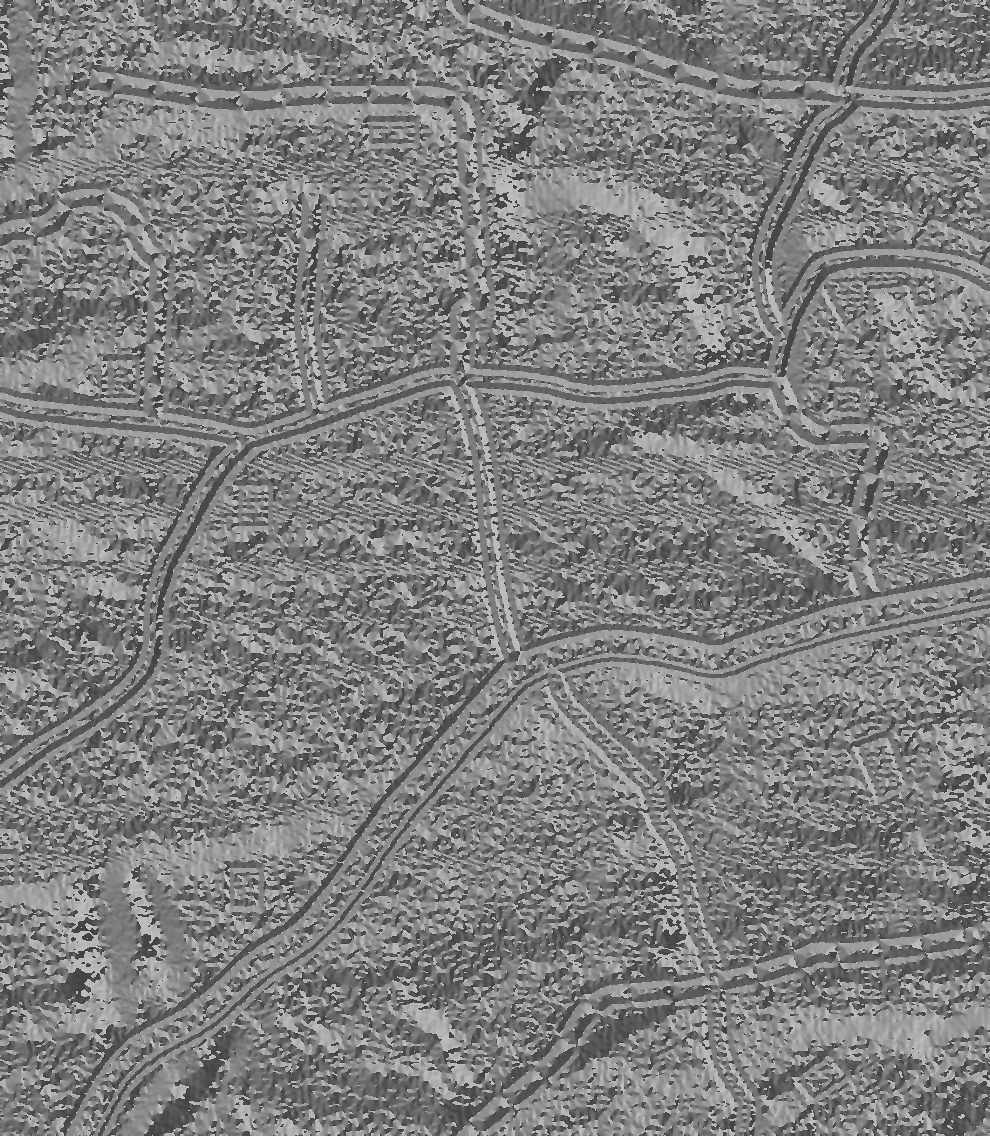
\includegraphics[width=5cm]{images/edgeDetectionPrototype/f.jpg}
            \caption{Gaussian Filter}
            \label{fig:proto_gradDir}
        \end{figure} \bk

        \paragraph{5. Gradient Magnitude Threshold} \mbox{} \\
        Once both the combined gradient and gradient directions have been calculate the next step in the process is working out which parts of the edge detected image are noise and which are not. In order to do this the combined gradients and the direction are taken into account and similar to before we build a kernel of the surrounding pixels of the image. The first part of this however is to convert the values in radians to values in degrees, to do this we run all through all values and convert them first. This can be seen \textit{Lines 372 through 377}.
        
        \begin{cscode}
public double[,] ConvertThetaToDegrees(double[,] thetaArray)
{
    double[,] result = new double[thetaArray.GetLength(0), thetaArray.GetLength(1)];
    for (int i = 0; i < thetaArray.GetLength(0); i++) for (int j = 0; j < thetaArray.GetLength(1); j++) result[i, j] = 180 * Math.Abs(thetaArray[i, j]) / Math.PI;
    return result;
}
        \end{cscode}
        
        Once all values are in degrees this becomes easier to deal with since there is less data lost to floating point arithmetic. Now that the angles are in degrees they are compared to predefined values as shown in the code. Depending which if the categories the pixel in question falls into the kernel is then used to decide whether that pixel will be set to black or not. Since this is the first filtering pass it is rather blunt and will not remove all of the noise in the image, this will come at a later stage through the use of min max threshold. Just so that the gradients can be visualised this is what is generated (adjusted to be visible and comprehensible for a human) see above \textit{figure \ref{fig:proto_gradDir}}. \\ \bk

        \begin{figure}[H]
            \centering
            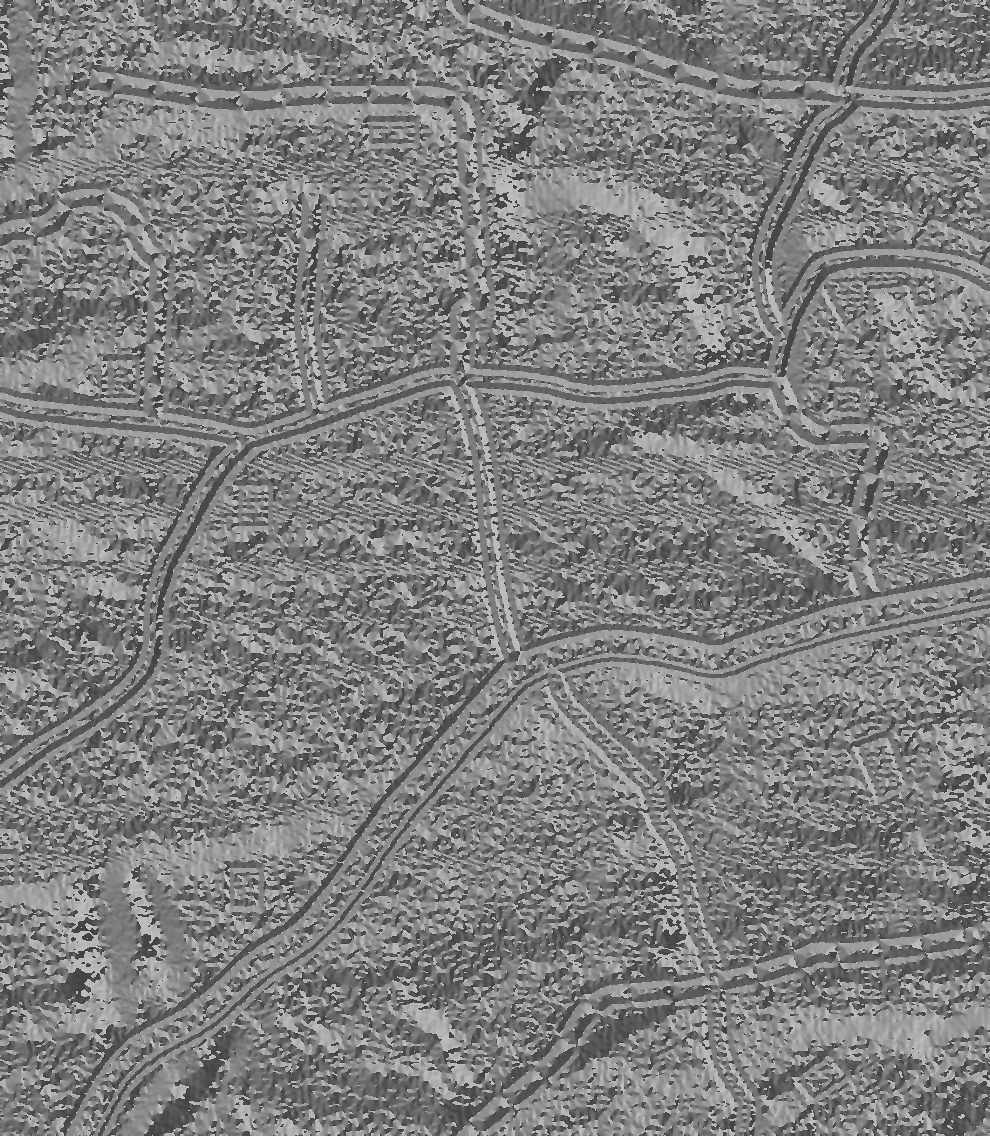
\includegraphics[width=5cm]{images/edgeDetectionPrototype/f.jpg}
            \caption{Gradient Direction}
            \label{fig:proto_gradDirection}
        \end{figure} \bk


        The part of the edge detection that this portion of the code is performing is removing parts of the image which have random lines and sporadic noise. This is due to us having a "direction" of where the gradient of the image is travelling. From this we can create a image kernel of our processed image so far. Depending on what the direction is it will fall into several categories. These can be seen in the code as follows:

        \begin{cscode}
public double[,] ApplyGradientMagnitudeThreshold(double[,] angles, double[,] magnitudes)
{
    double[,] result = magnitudes;
    double[,] anglesInDegrees = ConvertThetaToDegrees(angles);

    for (int i = 0; i < anglesInDegrees.GetLength(0); i++)
    {
        for (int j = 0; j < anglesInDegrees.GetLength(1); j++)
        {
            double[,] magnitudeKernel = BuildKernel(j, i, 3, magnitudes).matrix;

            if (anglesInDegrees[i, j] < 22.5 || anglesInDegrees[i, j] >= 157.5)
            {
                if (magnitudes[i, j] < magnitudeKernel[1, 2] || magnitudes[i, j] < magnitudeKernel[1, 0])
                {
                    result[i, j] = 0;
                }
            }
            else if (anglesInDegrees[i, j] >= 22.5 && anglesInDegrees[i, j] < 67.5)
            {
                if (magnitudes[i, j] < magnitudeKernel[0, 2] || magnitudes[i, j] < magnitudeKernel[2, 0])
                {
                    result[i, j] = 0;
                }
            }
            else if (anglesInDegrees[i, j] >= 67.5 && anglesInDegrees[i, j] < 112.5)
            {
                if (magnitudes[i, j] < magnitudeKernel[0, 1] || magnitudes[i, j] < magnitudeKernel[2, 1])
                {
                    result[i, j] = 0;
                }
            }
            else if (anglesInDegrees[i, j] >= 112.5 && anglesInDegrees[i, j] < 157.5)
            {
                if (magnitudes[i, j] < magnitudeKernel[0, 0] || magnitudes[i, j] < magnitudeKernel[2, 2])
                {
                    result[i, j] = 0;
                }
            }
            else throw new Exception();
        }
    }

    return result;
}
        \end{cscode}

        The use of the exception at the end is because the code above should catch all values however if it doesn't then something has gone wrong and therefore the process should not continue. After this has been applied to our image we are left with:
        
        \begin{figure}[H]
            \centering
            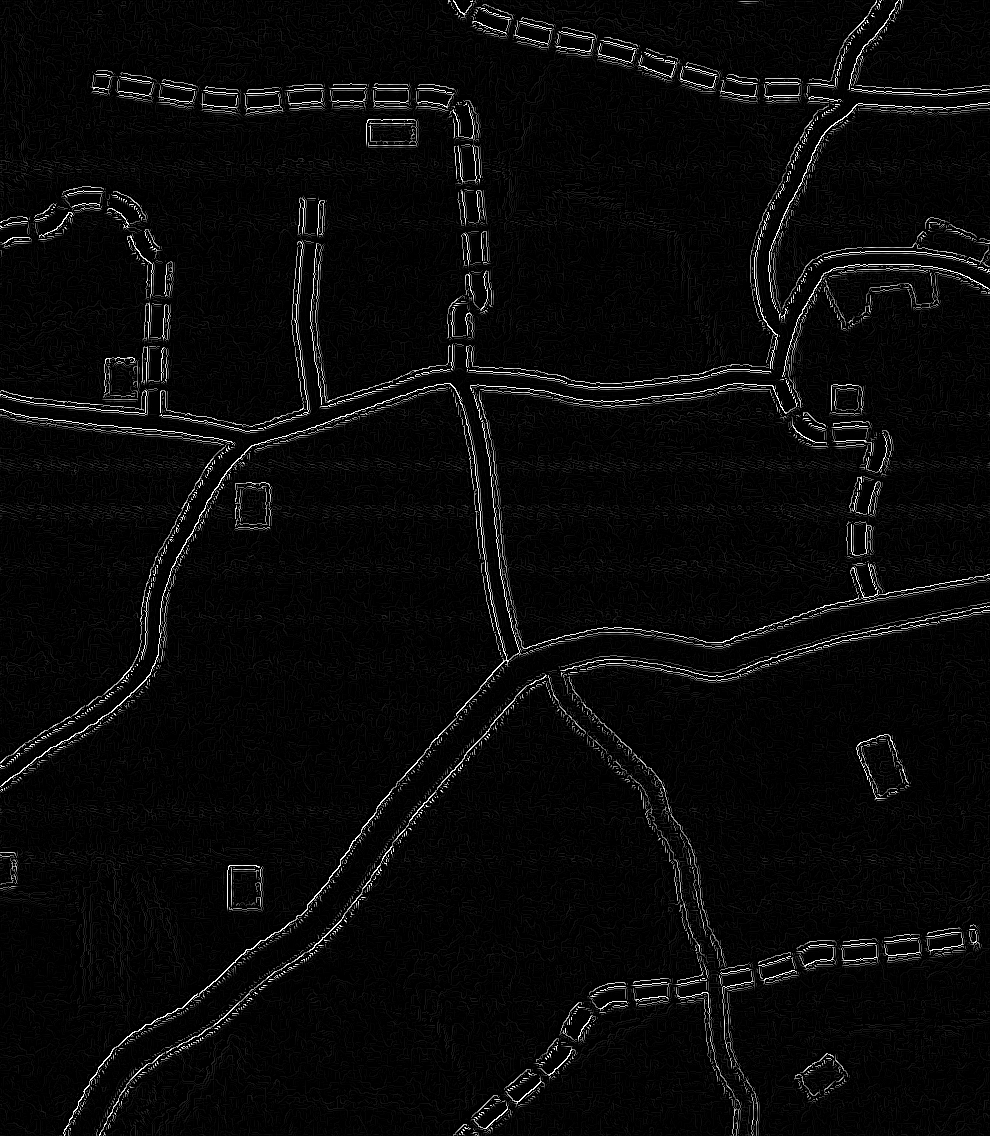
\includegraphics[width=5cm]{images/edgeDetectionPrototype/g.jpg}
            \caption{Magnitude Threshold}
            \label{fig:proto_magnitudeThreshold}
        \end{figure} \bk

        \paragraph{6. Min Max Threshold and Potential Edge Calculations} \mbox{} \\
        This part of the canny edge detection is also called the double threshold. This is where the image pixels will all be taken and their values considered. This is when it becomes necessary for us to use the black and white version of the image. If we did not then there would be no easy way to perform this. This is because unlike most of he other steps of the edge detection we are not interested yet at the pixels which are surrounding the ones we are looking at. We are just interested in its specific value. The code to perform this is as follows.

        \begin{cscode}
public (double, bool)[,] ApplyDoubleThreshold(double l, double h, double[,] gradients)
{
    double min = l * 255;
    double max = h * 255;

    (double, bool)[,] result = new (double, bool)[gradients.GetLength(0), gradients.GetLength(1)];

    for (int i = 0; i < gradients.GetLength(0); i++)
    {
        for (int j = 0; j < gradients.GetLength(1); j++)
        {
            if (gradients[i, j] < min) result[i, j] = (0, false);
            else if (gradients[i, j] > min && gradients[i, j] < max) result[i, j] = (gradients[i, j], false);
            else if (gradients[i, j] > max) result[i, j] = (gradients[i, j], true);
            else throw new Exception();
        }
    }

    return result;
}
        \end{cscode}

        The function takes two important parameters. The lower bound and the upper bound. These are the values at which we decide if a pixel is too weak and is to be set to black, if it is a "weak" pixel or a "strong" pixel. These are not important at the moment however will be used when it comes to hysteresis. Some pixels will be out right removed however and we can see the result of this double threshold is.

        \begin{figure}[H]
            \centering
            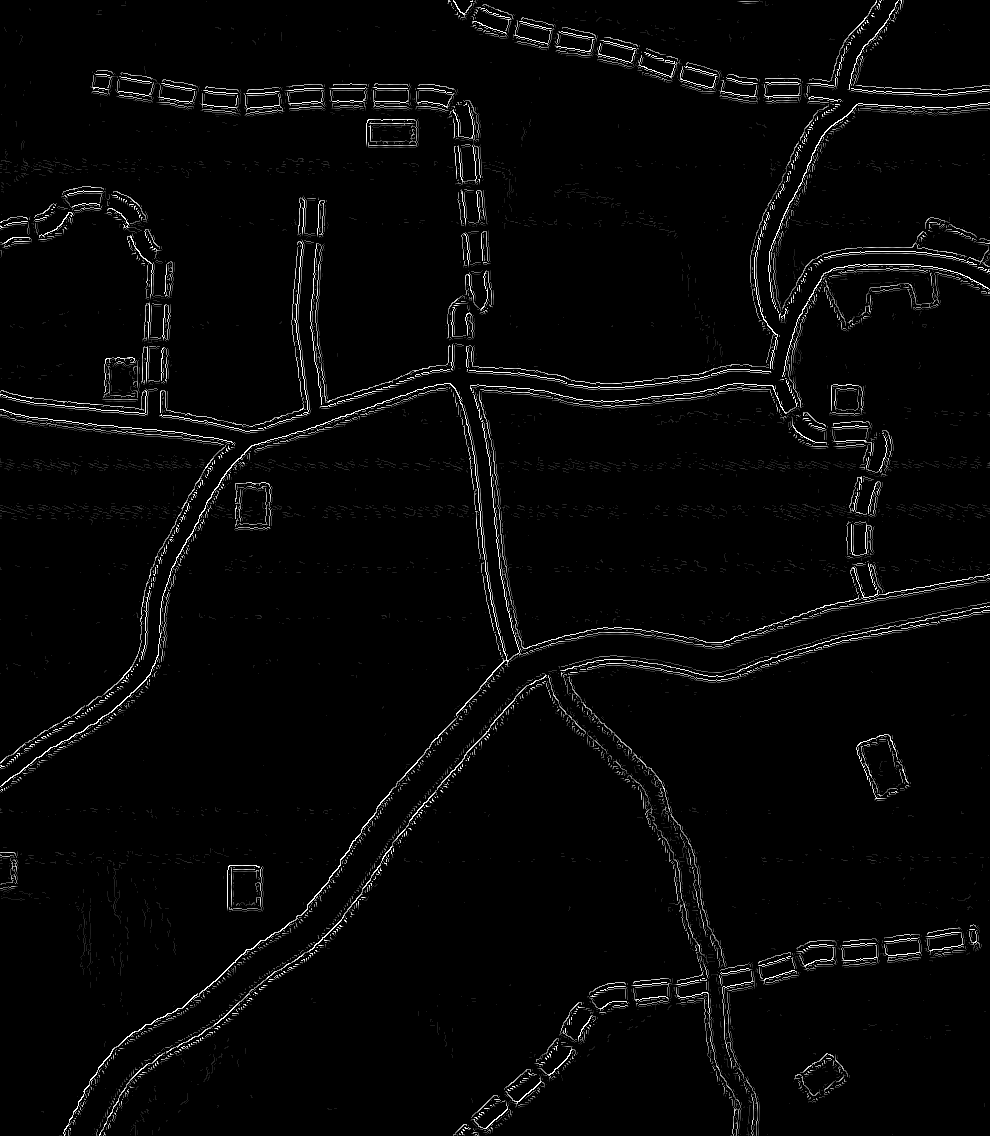
\includegraphics[width=5cm]{images/edgeDetectionPrototype/h.jpg}
            \caption{Magnitude Threshold}
            \label{fig:proto_minmaxThreshold}
        \end{figure} \bk

        As you can see lots of noise from the scan lines of the image have been removed in this step as they would have been too small to make it past the lower threshold. Now we have an 2D array of pixel values and whether they are considered "strong" or not. If they are strong this is represented by \textbf{true} in the $2\textsuperscript{nd}$ part of the tuple. And \textbf{false} for a "weak" pixel. \\ \bk

        \paragraph{7. Edge tracking by Hysteresis} \mbox{} \\
        This is the final step of traditional canny edge detection. This will require the 2D array of tuples and will require kernels of the image as it loops over every pixel. This will cause a problem since the usual way fo doing it would default to grey if the kernel overlapped with the edge of the image. So in this case we default to the pixel itself because any other value could cause us to get an erroneous edge. The way that this works is if the pixel is a "strong" pixel then it is defaulted to an edge since it was above the previous threshold. If the pixel is "weak" then it will build a kernel of all of the images around it. If any of the pixels which surround it are "strong" then this pixel is made "strong". The code for this is as follows.

        \begin{cscode}
public double[,] ApplyEdgeTrackingHysteresis((double, bool)[,] arrayOfValues)
{
    double[,] result = new double[arrayOfValues.GetLength(0), arrayOfValues.GetLength(1)];

    for (int i = 0; i < arrayOfValues.GetLength(0); i++)
    {
        for (int j = 0; j < arrayOfValues.GetLength(1); j++)
        {
            if (arrayOfValues[i, j].Item2 == false)
            {
                (double, bool)[,] imageKernel = BuildKernel(j, i, 3, arrayOfValues);
                bool strong = false;
                for (int k = 0; k < 3 && !strong; k++)
                {
                    for (int l = 0; l < 3 && !strong; l++)
                    {
                        if (imageKernel[k, l].Item2 == true) strong = true;
                    }
                }

                result[i, j] = strong ? 255 : 0;
            }
            else result[i, j] = 255;
        }
    }

    return result;
}
        \end{cscode}

        After this has been completed we are left with a classically edge detected image which looks as follows. The left image is the original for comparison purposes.

                
        \begin{figure}[H]
            \centering
            \subfloat[Original Input Image]{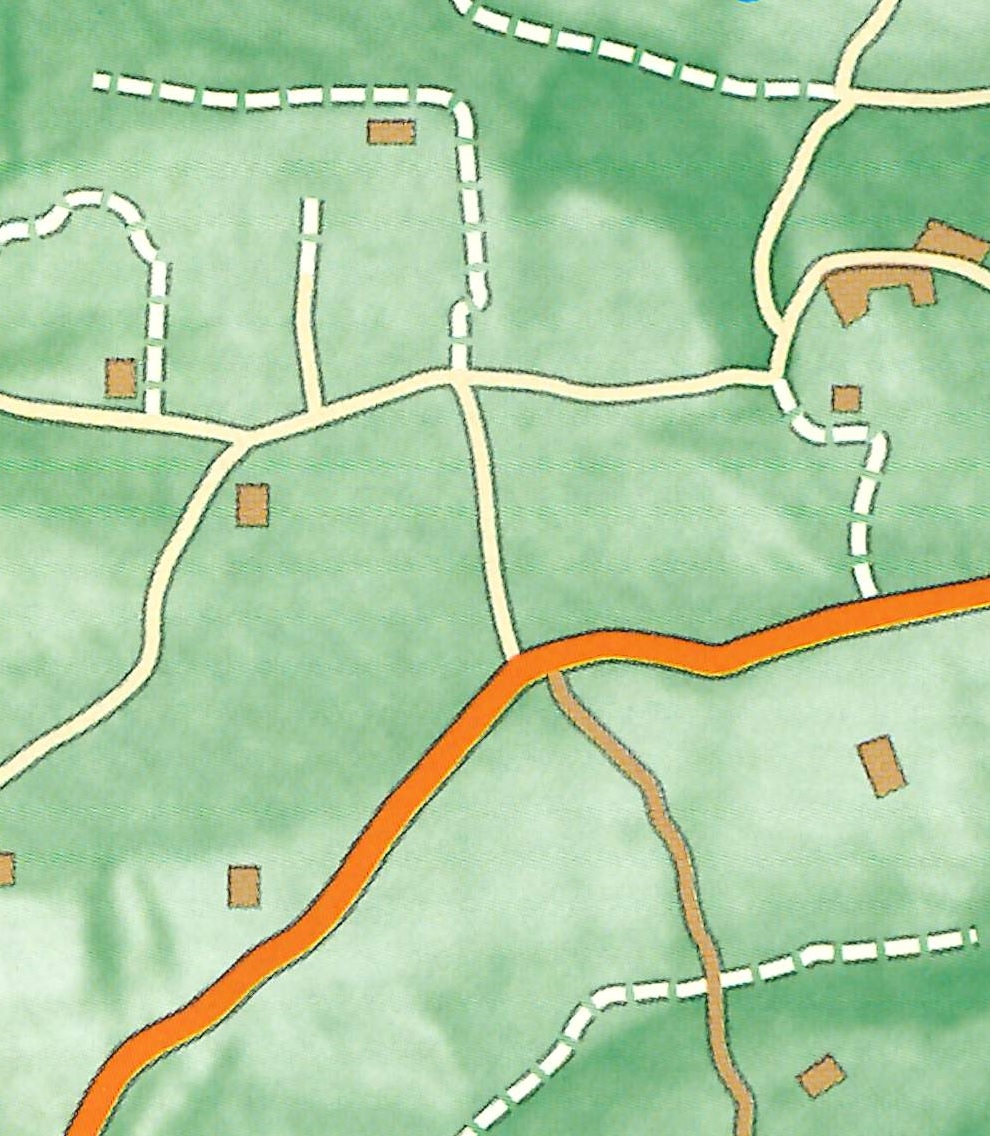
\includegraphics[width=5cm]{images/edgeDetectionPrototype/in.jpg}}
            \label{fig:proto_originalComaprison}
            \qquad
            \subfloat[Image after Classic Edge Detection]{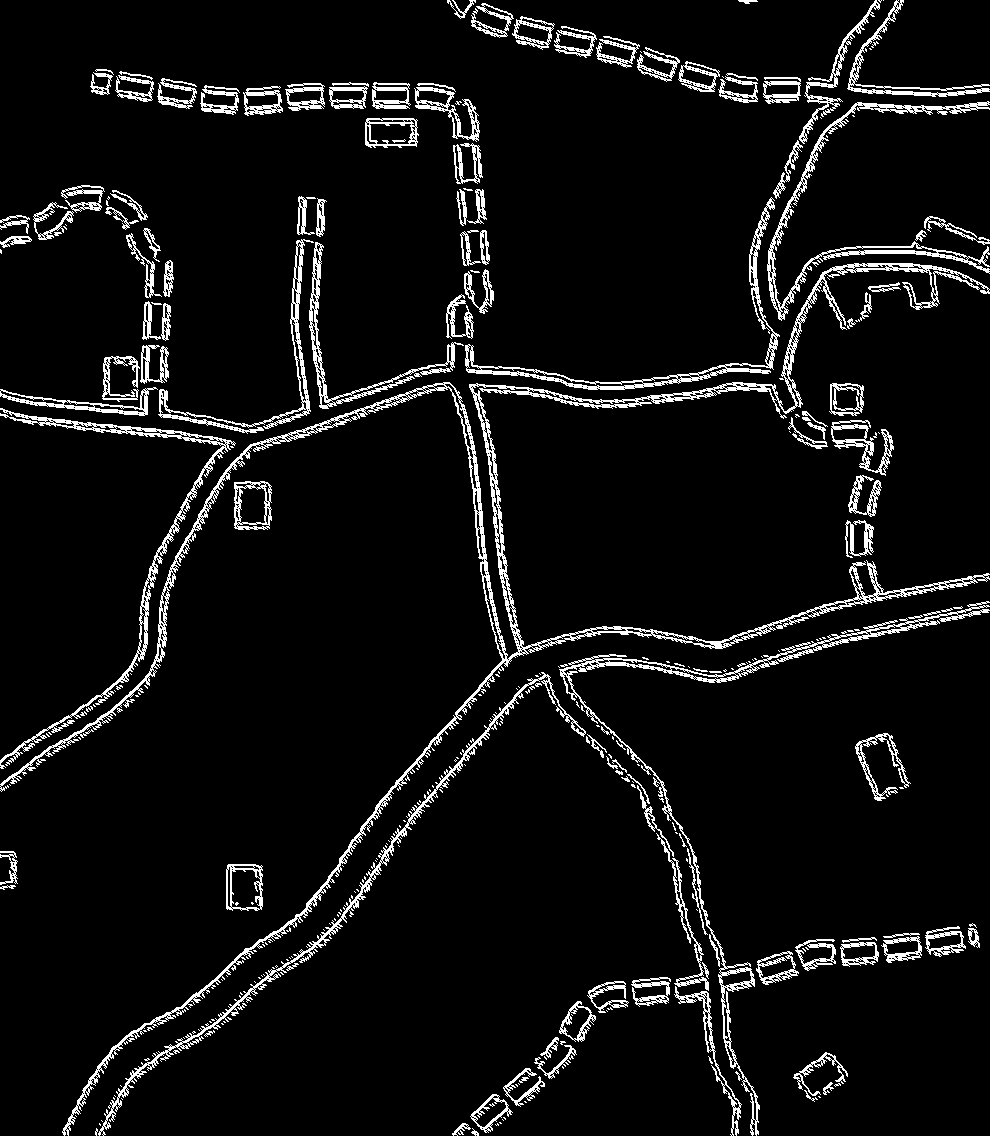
\includegraphics[width=5cm]{images/edgeDetectionPrototype/i.jpg}}
            \label{fig:proto_hysteresis}
        \end{figure} \bk

        As is visible in the final image we can see that after the edge detection there are holes in the lines. As well as this there are occasional gaps this is where I came up with a extra couple of steps. This allows the image to be properly formed and connect any miscellaneous roads which have small gaps.

        \paragraph{8. Emboss Kernel} \mbox{} \\
        This stage isn't strictly needed for more than the reasons stated above, this will make it so that the some roads which are slightly separated, or artifacts left over from the edge detection are removed. This is done thought the use of an image kernel which is as follows: \\ 

        \begin{gather*}
            \begin{pmatrix}
                -2 & -1 & 0 \\
                -1 & 1  & 1 \\
                0  & 1  & 2 \\
            \end{pmatrix}
        \end{gather*}

        The code for this is very simple and involved convolution across the entire image using this code. \\ \bk

        \begin{cscode}
public double[,] EmbossImage(double[,] imageArray)
{
    double[,] result = new double[imageArray.GetLength(0), imageArray.GetLength(1)];

    Matrix embossMatrix = new Matrix(new double[,]
    {
        { -2, -1, 0 },
        { -1, 1, 1 },
        { 0, 1, 2 },
    });

    for (int i = 0; i < imageArray.GetLength(0); i++)
    {
        for (int j = 0; j < imageArray.GetLength(1); j++)
        {
            Matrix imageKernel = BuildKernel(j, i, 3, imageArray);
            result[i, j] = Math.Abs(Matrix.Convolution(imageKernel, embossMatrix));
        }
    }

    return result;
}
        \end{cscode}

        This results in, as you can imagine, an embossed image. \\ \bk

        \begin{figure}[H]
            \centering
            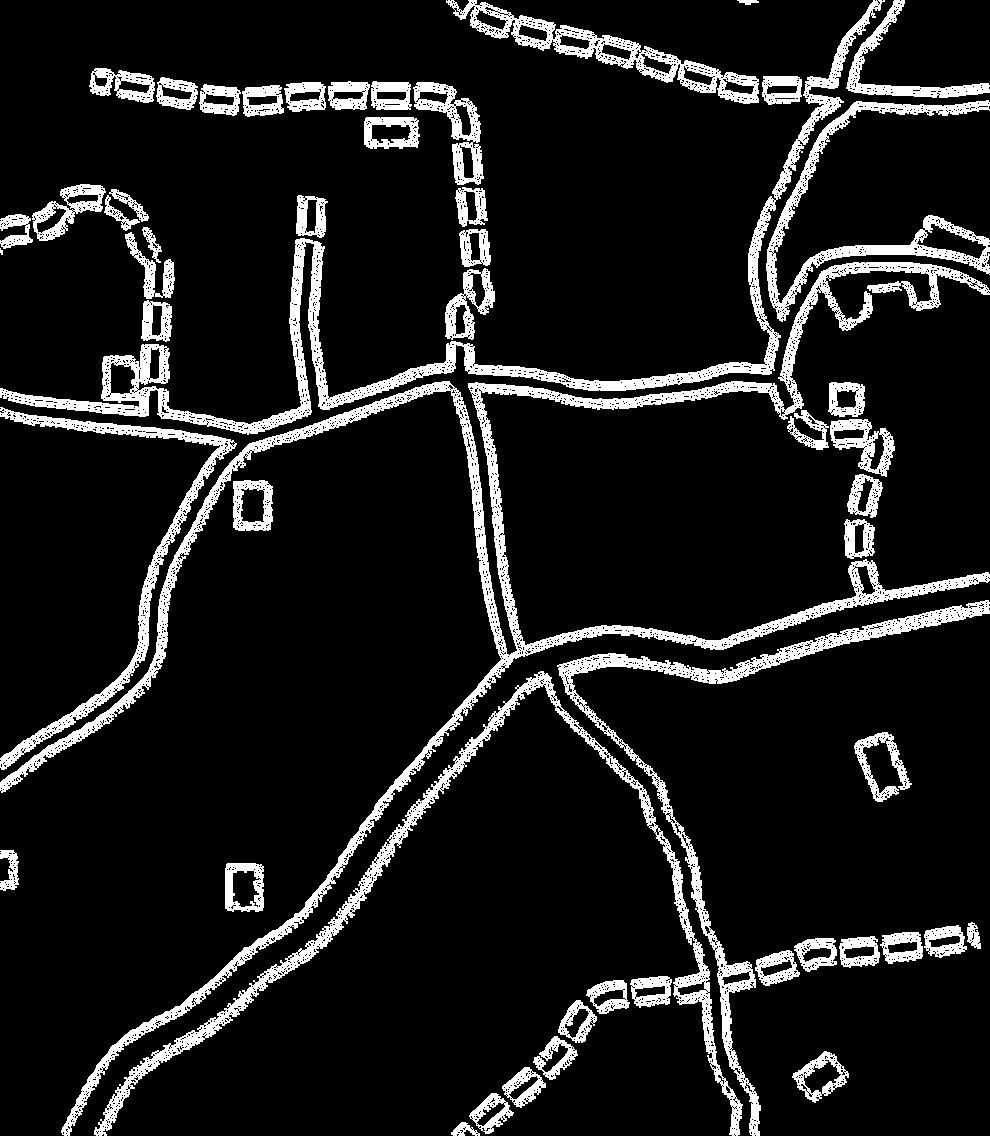
\includegraphics[width=5cm]{images/edgeDetectionPrototype/j.jpg}
            \caption{Magnitude Threshold}
            \label{fig:proto_embossedImage}
        \end{figure} \bk

        \paragraph{9. Custom Hole Filling} \mbox{} \\
        Now that the lines of the image have been increased then the only step which remains is to make the lines full and complete, this means that in the future when this is Incorporated into my final solution when a filling algorithm is applied it wont pick up erroneous roads.
        
        \begin{figure}[H]
            \centering
            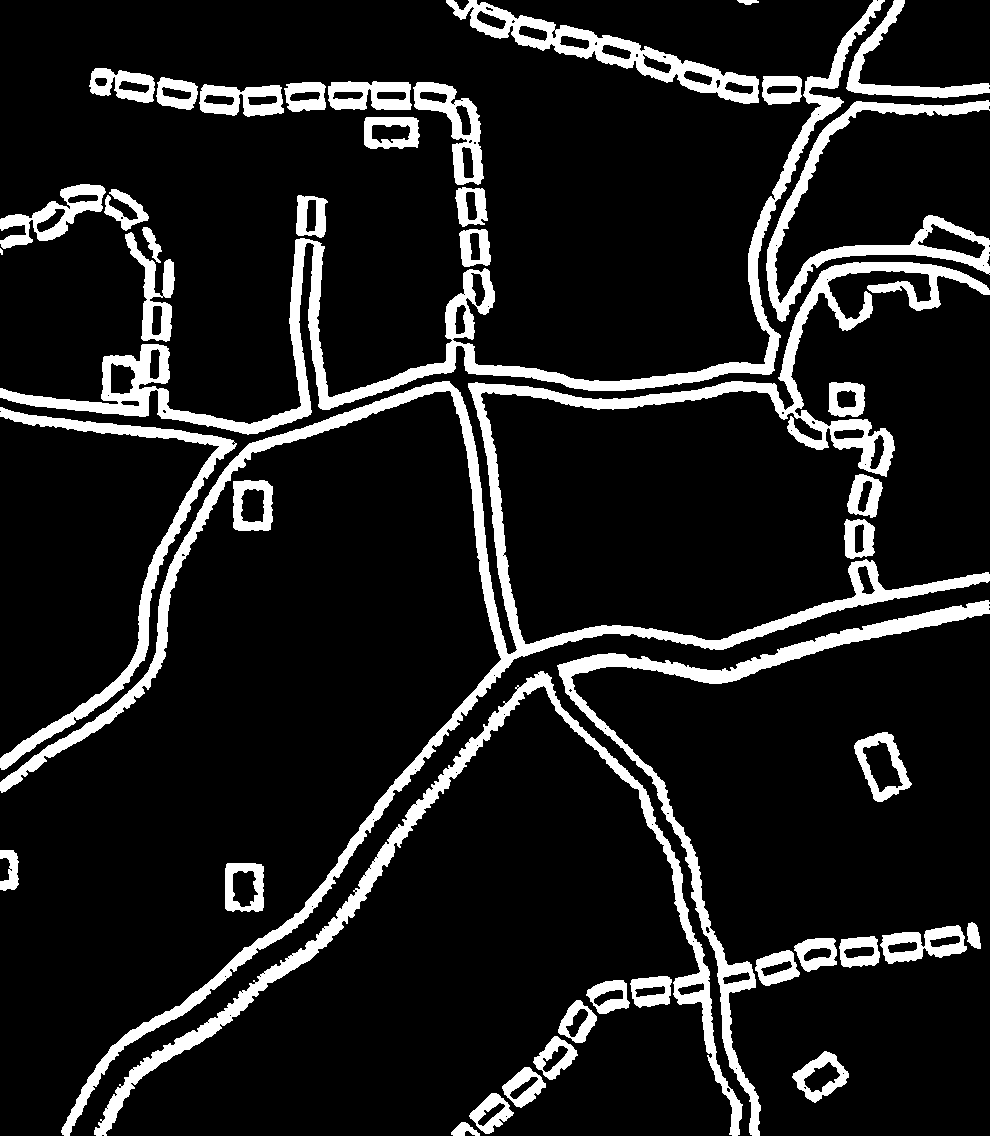
\includegraphics[width=5cm]{images/edgeDetectionPrototype/k.jpg}
            \caption{Magnitude Threshold}
            \label{fig:proto_finalFilledImage}
        \end{figure} \bk

        This is completed with the following code, the way that it works is that it takes a kernel of the surrounding image. If there is a certain amount of pixels in the surrounding kernel which are white then the center pixel is set to white. This threshold can be changed but 4 works well. 

        \begin{cscode}
public double[,] FillImage(double[,] imageArray)
{
    double[,] result = imageArray;

    for (int i = 0; i < imageArray.GetLength(0); i++)
    {
        for (int j = 0; j < imageArray.GetLength(1); j++)
        {
            Matrix imageKernel = BuildKernel(j, i, 3, imageArray);
            int count = 0;
            foreach (double value in imageKernel.matrix)
            {
                if (value >= 255) count++;
            }

            if (count > 4) result[i, j] = 255;
        }
    }

    return result;
}
        \end{cscode}


        \subsubsection{Graph Class and Graph Traversal}
        The graph data structure is well documented and has two main ways of being represented. One of which is a Adjacency List and the other is an Adjacency Matrix, each have their advantages and disadvantages so I will start with those.

        \begin{enumerate}
            \item Adjacency Matrix
            \begin{itemize}
                \item Advantages
                    \begin{enumerate}
                        \item[] Very fast when needing to lookup connections.
                        \item[] Inserting is also fast due to it being instantly accessible and not a dynamic structure.
                    \end{enumerate}
                \item Disadvantages
                \begin{enumerate}
                        \item[] Very memory inefficient and will need to grow exponentially in each dimension with the amount of pixels in the image.
                        \item[] When you have a sparse graph it is even more inefficient.
                \end{enumerate}
            \end{itemize}
            \item Adjacency List
                \begin{itemize}
                    \item Advantages
                    \begin{enumerate}
                        \item[] Easier to use pragmatically and implement
                        \item[] It is much easier to use Linq functions with to find graph connections
                    \end{enumerate}
                    \item Disadvantages
                    \begin{enumerate}
                        \item[] Relatively slower when it comes to accessing sections of the graph.
                        \item[] Would have to be a hybrid with a dictionary to allow for reasonable use
                    \end{enumerate}
            \end{itemize}.
        \end{enumerate}

        With all of this being said I decided to go for a Dictionary List since this was the easiest way to programmatically manipulate it. It also makes it easier to enter a new graph. This compared to a matrix where it would get into extreme values quickly. The structure of my prototype graph is: \\ \bk

       \begin{figure}[H]
            \centering
            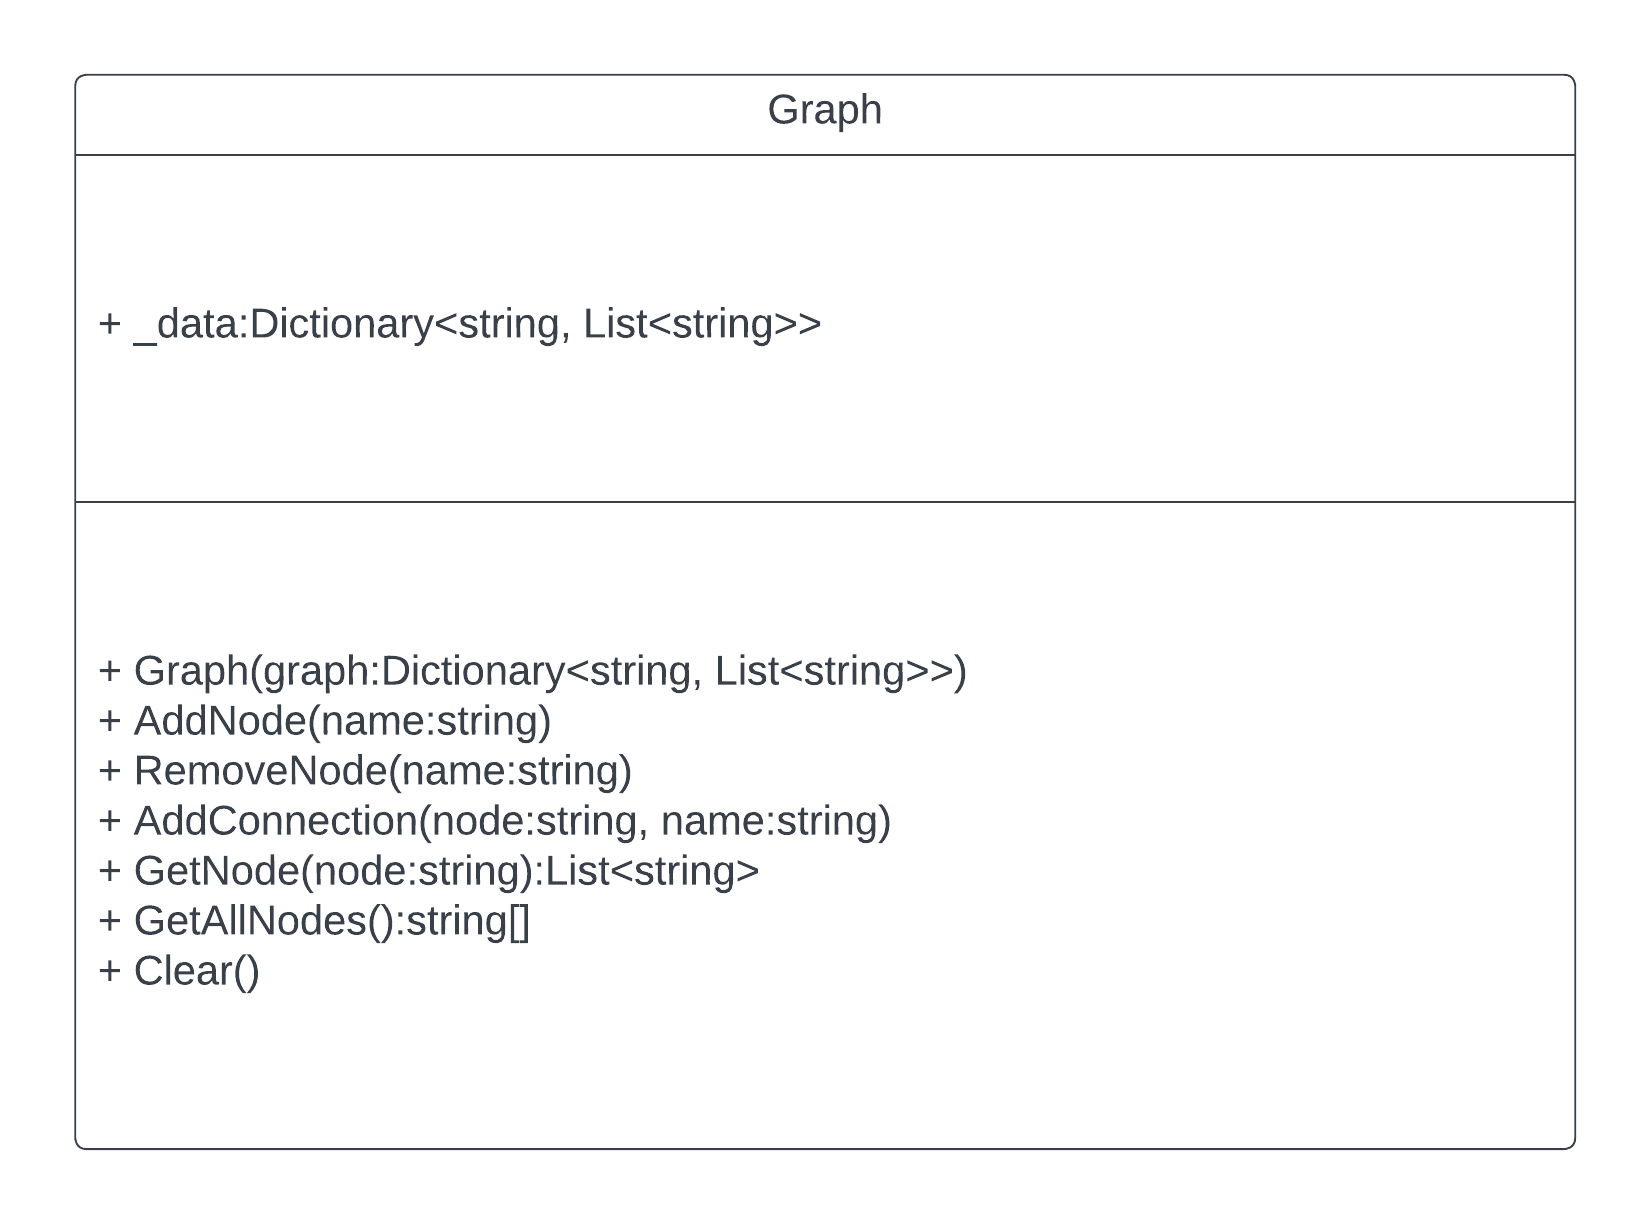
\includegraphics[width=10cm]{images/graphClassDiagram.png}
            \caption{Graph UML Diagram}
            \label{fig:proto_umlGraph}
        \end{figure} \bk

        and in code \\ \bk

        \begin{cscode}
public class Graph
{
    public Dictionary<string, List<string>> _data = new Dictionary<string, List<string>>();

    public Graph(Dictionary<string, List<string>> graph)
    {
        _data = graph;
    }

    public void AddNode(string name)
    {
        if (_data.ContainsKey(name)) throw new GraphException($"Cannot add {name}, node already exists.");
        _data.Add(name, new List<string>());
    }

    public void RemoveNode(string name)
    {
        if (!_data.ContainsKey(name)) throw new GraphException($"Cannot remove {name}, node does not exist.");
        _data.Remove(name);
    }

    public void AddConnection(string node, string name)
    {
        if (!_data.ContainsKey(node)) throw new GraphException($"Cannot add connection {name} to {node} original node does not exist.");
        if (_data[node].Contains(name)) throw new GraphException($"Cannot add connection {name} to {node} connection already exists.");
        _data[node].Add(name);
    }

    public List<string> GetNode(string node)
    {
        if (!_data.ContainsKey(node)) throw new GraphException($"Node {node} does not exist.");
        return _data[node];
    }

    public string[] GetAllNodes() => _data.Keys.ToArray();

    public void Clear() => _data.Clear();
}
        \end{cscode}

        This is the most basic of graph structures and may need to be changed as I develop the final solution however for the moment it serves as a good prototype. With this graph I also went on to program basic DFS (Depth-First Search) and BFS (Breadth First Search). \\ \bk

        \begin{cscode}
public static string[] DFS(string start, Graph graph)
{
    List<string> path = new List<string>();
    Stack<string> stack = new Stack<string>();
    Dictionary<string, bool> visited = new Dictionary<string, bool>();
    foreach (string s in graph.GetAllNodes()) visited.Add(s, false);

    // Kick Start
    stack.Push(start);

    while (!stack.IsEmpty())
    {

        string node = stack.Pop();
        path.Add(node);
        visited[node] = true;

        List<string> connections = graph.GetNode(node);

        connections.Reverse();

        foreach (string s in connections)
        {
            if (visited[s] == false)
            {
                stack.Push(s);
            }
        }
    }


    return path.ToArray();
}

public static string[] BFS(string start, Graph graph)
{
    List<string> path = new List<string>();
    Queue<string> stack = new Queue<string>();
    Dictionary<string, bool> visited = new Dictionary<string, bool>();
    foreach (string s in graph.GetAllNodes()) visited.Add(s, false);

    // Kick Start
    stack.Enqueue(start);

    while (!stack.IsEmpty())
    {

        string node = stack.Dequeue();
        path.Add(node);
        visited[node] = true;

        List<string> connections = graph.GetNode(node);

        connections.Reverse();

        foreach (string s in connections)
        {
            if (visited[s] == false)
            {
                stack.Enqueue(s);
            }
        }
    }

    return path.ToArray();
}
        \end{cscode}

        Both of these I ran through by hand and they came out correct. It was useful to see how they are calculated and how the implementation is different depending on whether you use a stack or a queue for the graph traversal.
        
        \subsubsection{Windows Forms with Images}
        To allow the user to easily be able to see the output of the edge detection. In order to do this the project needed to be created in dot-Net Framework. Once this is done a basic mock up of what the prompt to the user will see is made in the user interface. This creates backend XML which is interpreted by the framework to be presented to the user. As well as this there is also the programmatic part to it which can be used to display the image. \\ \bk
        
        \textbf{Example}

        \begin{cscode}
partial class ShowImage
{
    /// <summary>
    /// Required designer variable.
    /// </summary>
    private System.ComponentModel.IContainer components = null;

    /// <summary>
    /// Clean up any resources being used.
    /// </summary>
    /// <param name="disposing">true if managed resources should be disposed; otherwise, false.</param>
    protected override void Dispose(bool disposing)
    {
        if (disposing && (components != null))
        {
            components.Dispose();
        }
        base.Dispose(disposing);
    }

    #region Windows Form Designer generated code

    /// <summary>
    /// Required method for Designer support - do not modify
    /// the contents of this method with the code editor.
    /// </summary>
    private void InitializeComponent()
    {
        this.imageBox = new System.Windows.Forms.PictureBox();
        this.next = new System.Windows.Forms.Button();
        this.content = new System.Windows.Forms.RichTextBox();
        ((System.ComponentModel.ISupportInitialize)(this.imageBox)).BeginInit();
        this.SuspendLayout();
        // 
        // imageBox
        // 
        this.imageBox.Location = new System.Drawing.Point(12, 12);
        this.imageBox.Name = "imageBox";
        this.imageBox.Size = new System.Drawing.Size(500, 450);
        this.imageBox.TabIndex = 1;
        this.imageBox.TabStop = false;
        // 
        // next
        // 
        this.next.Font = new System.Drawing.Font("JetBrains Mono SemiBold", 24.75F, System.Drawing.FontStyle.Bold, System.Drawing.GraphicsUnit.Point, ((byte)(0)));
        this.next.Location = new System.Drawing.Point(518, 384);
        this.next.Name = "next";
        this.next.Size = new System.Drawing.Size(354, 78);
        this.next.TabIndex = 4;
        this.next.Text = "Continue";
        this.next.UseVisualStyleBackColor = true;
        this.next.Click += new System.EventHandler(this.next_Click);
        // 
        // content
        // 
        this.content.AcceptsTab = true;
        this.content.Font = new System.Drawing.Font("JetBrains Mono SemiBold", 15F, System.Drawing.FontStyle.Bold);
        this.content.Location = new System.Drawing.Point(518, 12);
        this.content.Name = "content";
        this.content.ReadOnly = true;
        this.content.Size = new System.Drawing.Size(354, 366);
        this.content.TabIndex = 5;
        this.content.Text = "";
        // 
        // ShowImage
        // 
        this.AutoScaleDimensions = new System.Drawing.SizeF(6F, 13F);
        this.AutoScaleMode = System.Windows.Forms.AutoScaleMode.Font;
        this.ClientSize = new System.Drawing.Size(884, 474);
        this.Controls.Add(this.content);
        this.Controls.Add(this.next);
        this.Controls.Add(this.imageBox);
        this.Name = "ShowImage";
        this.Text = "ShowImage";
        this.Load += new System.EventHandler(this.ShowImage_Load);
        ((System.ComponentModel.ISupportInitialize)(this.imageBox)).EndInit();
        this.ResumeLayout(false);

    }

    #endregion

    private System.Windows.Forms.PictureBox imageBox;
    private System.Windows.Forms.Button next;
    private System.Windows.Forms.RichTextBox content;
}
        
public partial class ShowImage : Form
{
    private Bitmap _image;
    private string _content;

    public ShowImage(Bitmap image, string content)
    {
        this.ControlBox = false;

        _image = image;
        _content = content;

        InitializeComponent();
    }

    private void ShowImage_Load(object sender, EventArgs e)
    {
        imageBox.SizeMode = PictureBoxSizeMode.StretchImage;
        imageBox.Image = _image;
        content.Text = _content;
    }

    private void next_Click(object sender, EventArgs e)
    {
        Close();
    }
}
        \end{cscode}

        These two partial classes come together to form the final form. One thing which I learned from this prototype is that there are several ways that the image can be made to fill the text box and that needs to be carefully considered.
            

        \subsection{Objectives}
        \normalsize
        
        % Tips for objectives
        
        % 1. Use numbered objectives to allow them to be refer ed back to
        % 2. Don't mention programming techniques
        % 3. Objectives for the program not the programmer
        
        After conducting the initial and second interviews and reflecting upon the results of my research I have formed a list of objectives that the program must meet to be considered 
        complete. As well as the base objectives I have also, with help from my end user, come up with extensions which will increase the effectiveness of my solution overall. \\
        \bk
        
        \renewcommand{\labelenumii}{\arabic{enumi}.\arabic{enumii}}
        \renewcommand{\labelenumiii}{\arabic{enumi}.\arabic{enumii}.\arabic{enumiii}}
        \renewcommand{\labelenumiv}{\arabic{enumi}.\arabic{enumii}.\arabic{enumiii}.\arabic{enumiv}}
        
        \begin{enumerate}
            \item The Program must have way to input a Map
            \begin{enumerate}
                \item The Program should be able to parse a map from a file, including
                \begin{enumerate}
                    \item A photograph of an map
                    \item A screenshot of an existing map
                    \item A hand drawing of suitable quality (if it is not a message should be shown)
                \end{enumerate}
                \item When the user inputs a map, the program will ask them
                \begin{enumerate}
                    \item What type of map they are inputting
                    \item Whether this is the correct image
                    \item Whether they want the image deleted after edge detection
                    \item Whether they would like the image to be stored in a binary file, \\
                    \begin{enumerate}
                        \item If selected then the programs should ask for a name
                        \item It should ask for a description of the image
                        \item It should ask for the type of image.
                        \item The time and date of the image should be automatically calculated.
                    \end{enumerate}
                    \emph{These are just some examples of prompts}
                \end{enumerate}
                \item The inputted map should be converted into a graph
                \begin{enumerate}
                    \item The map (in graph form) should be able to be traversed
                    \item The map in graph form should be simplified to ensure that redundant nodes are not recorded.
                \end{enumerate}
                
                \item If any error occurs during the map input process an appropriate error should be displayed and the program should continue to run
            \end{enumerate}

            \item The Program must perform canny edge detection   
            \begin{enumerate}
                \item At each stage of the edge detection an image should be produced
                \begin{enumerate}
                    % \item The user should be able to save the intermediate images.
                \end{enumerate}
                \item Between each stage the user should be able to repeat the last step in order to change parameters.\\
                \emph{The user should be able to change (at various stages):} 
                \begin{enumerate}
                    \item The sigma value of the Gaussian elimination
                    \item The lower threshold value
                    \item The higher threshold value
                    \item The Gaussian kernel size
                    \item The black and white filter ratios
                    \item The amount of times embossing is performed
                    \item The times de-blocking should be performed
                \end{enumerate}
                \item The edge detection must have the option to be multi threaded.
                \begin{enumerate}
                    \item There should be presets to allow quicker processing
                    \begin{enumerate}
                        \item There should be a preset for hand drawn images
                        \item There should be a preset for photographed images
                        \item There should be a preset for screen shot images
                    \end{enumerate}
                \end{enumerate}
                
                \item The edge detection must have the option to be single threaded
            \end{enumerate}
            
            \item The Program must overlay the detected roads onto the original image
            \begin{enumerate}
                \item The result of the edge detection will be shown to the user before road detection
                \item The program will perform road detection
                \begin{enumerate}
                    \item The image should have the option to be inverted
                    \item A filling algorithm should be applied to the image
                    \item The percentage threshold for non roads much be changeable by the user
                    \item The total filled image can be displayed to the user
                    \item The singled out roads and paths must be shown to the user
                \end{enumerate}
                
            \end{enumerate}
            
            \item The Program must allow Map Traversal
            \begin{enumerate}
                \item There should be Multiple Traversal Algorithms Available to be chosen from.
                    \begin{enumerate}
                        % https://en.wikipedia.org/wiki/Category:Graph_algorithms
                        \item The Program should implement Routing Algorithms 
                        \begin{enumerate}
                            \item This includes Dijkstra's algorithm
                            \item This includes A*
                        \end{enumerate}
                        % https://en.wikipedia.org/wiki/Category:Search_algorithms
                        \item The Program should Implement Searching Algorithms these do not have to be shown to the user.
                        \begin{enumerate}
                            \item This includes BFS (Breadth-first search).
                            \item This includes DFS (Depth-first search).
                        \end{enumerate}
                    \end{enumerate}
                \item Depending on the option that the user chooses they can either
                \begin{enumerate}
                    \item Decide a specific algorithm to use
                    \begin{enumerate}
                        \item The general efficiency should be displayed.
                        \item The general length of each should be displayed.
                        \item The node count of each should be displayed if Dijkstra's is selected.
                    \end{enumerate}
                \end{enumerate}
            \end{enumerate}
            
            \item The Program must have a Clear and Simplistic GUI.
            \begin{enumerate}
                \item At a glance the user should be able to ascertain which step they are at in the process.
                \item Whenever a forms is displayed it should not serve more than one purpose.
                \item There should be a setting so that if the user chooses more detail can be displayed.
                \item The main user window should not be cluttered with old information.
            \end{enumerate}          

            \item The program must implement abstract data types
            \begin{enumerate}
                \item The program must implement a matrix class
                \begin{enumerate}
                    \item The program must be able to perform basic operations
                    \begin{enumerate}
                        \item Perform matrix multiplication
                        \item Perform matrix addition
                        \item Perform matrix subtraction
                        \item Perform scalar multiplication
                        \item Perform matrix minimization
                \end{enumerate}
                \item The program must be able to find the determinant of a matrix
                \item The program must be able to find the inverse of a matrix
                \item The program must be able to apply the convolution operation
                \end{enumerate}
                \item The program should implement a graph class
                \begin{enumerate}
                    \item The graph should be able to be modified by
                    \begin{enumerate}
                        \item Inserting Nodes
                        \item Accessing per node
                        \item Access all nodes 
                        \item Inserting connections between nodes
                    \end{enumerate}
                    \item It should be implemented using an adjacency list.
                \end{enumerate}
            \end{enumerate}
            \bk
        \end{enumerate}  
        \vspace{1cm}    
        \centerline{\large\textbf{Extension Objectives}}
        \vspace{1cm}

        \begin{enumerate}[resume]
            \item The program should be able to output
            \begin{enumerate}
                \item The map in a binary file format
                \begin{enumerate}
                    \item This file can be saved
                    \item This file can be re-read and re-routed
                \end{enumerate}
                \item The saved images from the processing of the map should be able to be saved in a compressed format.
                \item The routed map with path drawn on it
                \item The saved binary file should be able to be cloned
                \item The saved binary file should be able to be renamed
                \item The saved binary file should be able to be have its description changed
                \item The saved binary file should be able to be able to be deleted                
            \end{enumerate}
            \item The program should have re-callable settings
            \begin{enumerate}
                \item Map Algorithm
                \item Random Save Names
                \item Map Approximations
            \end{enumerate}
            \item The program settings should be easily movable.
            \item The program save files should be easily movable.
        \end{enumerate}

        \bk

        % sufficiently well modelled ti be of use in subsequent stages
        % Outline the structure of the program
        % not all modeling needs to go in this section
        % class diagram and equations to be used
        % mockup of the interface (less vital)
        \subsection{Modelling}
            TODO
        \bk

\end{flushleft}

    \begin{flushleft}
    \normalsize
    \section{Technical Design}

    \subsection{Programming Language Selection and Libraries Used}

    I selected C# as my programming language for several reasons. Currently, it is the language that I am most familiar with. In addition, I conducted research on which languages are best for fast processing, and found that C, C++, and C# are among the top contenders. Considering my skill set and the importance of speed in this situation, I concluded that C# would be a good fit. Furthermore the object orientated nature of the language means that I will be able to separate the front end and the back end processing into separate bll files keeping the code clean and easily maintainable.\\ 
    \bk
    Find below a list of all libraries I used: \\
    
    \subsubsection{Linq}
    In order to manipulate lists and create the data structures that I need I will need to use some Linq methods. During the prototyping stage I found that using some Linq methods such as the Select statement allowed the program to be easier to read and make logical sense. As well as this there have been optimisations made in the iterative Linq methods which will make my program faster. Similar to some of the following libraries this is a Microsoft Library which is open source.
    \\ \bk


    \subsubsection{Bitmap}
    In order for my program to function a required part of it is that it is able to take an image as an input. In native C# there is no set way to do this. Therefore I needed to use the Microsoft System.Drawing Namespace. This namespace provides access to GDI+ basic graphics functionality. This does limit this project as is to only working on Windows since the library requires access to the GDI+ native library which is only on windows services. \\
    
    The only part of this library I will be using is the Bitmap class. This will allow me to accept all types of images without the need of parsing them myself since this is not the aim of my project. 
    \\ \bk

    \subsubsection{Windows Forms}
    In order to complete my objectives my program will need to be easy to use and any user with some degree of technical competency should be able to use it. In order to achieve this objective I though that instead of using some form of console input in order to get a starting and an end location, that it would be better to use some form of GUI. In order to do this I will use Windows Forms. This will allow me to make a simple GUI which will allow the end user to interact with the user and easily understand. \\ 

    The things which I will end up using the windows forms are the map traversal, allowing the user to select a start and an end node with a click instead of having to enter a coordinate. As well as this I will also use forms to show the user the stages of, for example, the canny edge detection.
    \\ \bk

    \subsection{High Level Overview}
    The general purpose of my project is to allow a user to take a map and input it into my program, then subsequently convert it into a routable map. \\ \bk
    
    In order to achieve this goal my program will first take an input, the users map. It will then take this map and convert it into an machine readable format, a Bitmap. Canny edge detection will then be performed on it causing the edges and the surroundings of the paths on the image to be found. Using these edges a filling algorithm will fill the spaces encapsulated by the lines. Finally these filled spaces will be used to convert the whole image to a graph which can then be traversed using graph traversal algorithms such as A* or Dijkstra's algorithm. \\ \bk

    \begin{figure}[H]
        \centering
        \subfloat[\centering High Level Overview Of Program]{{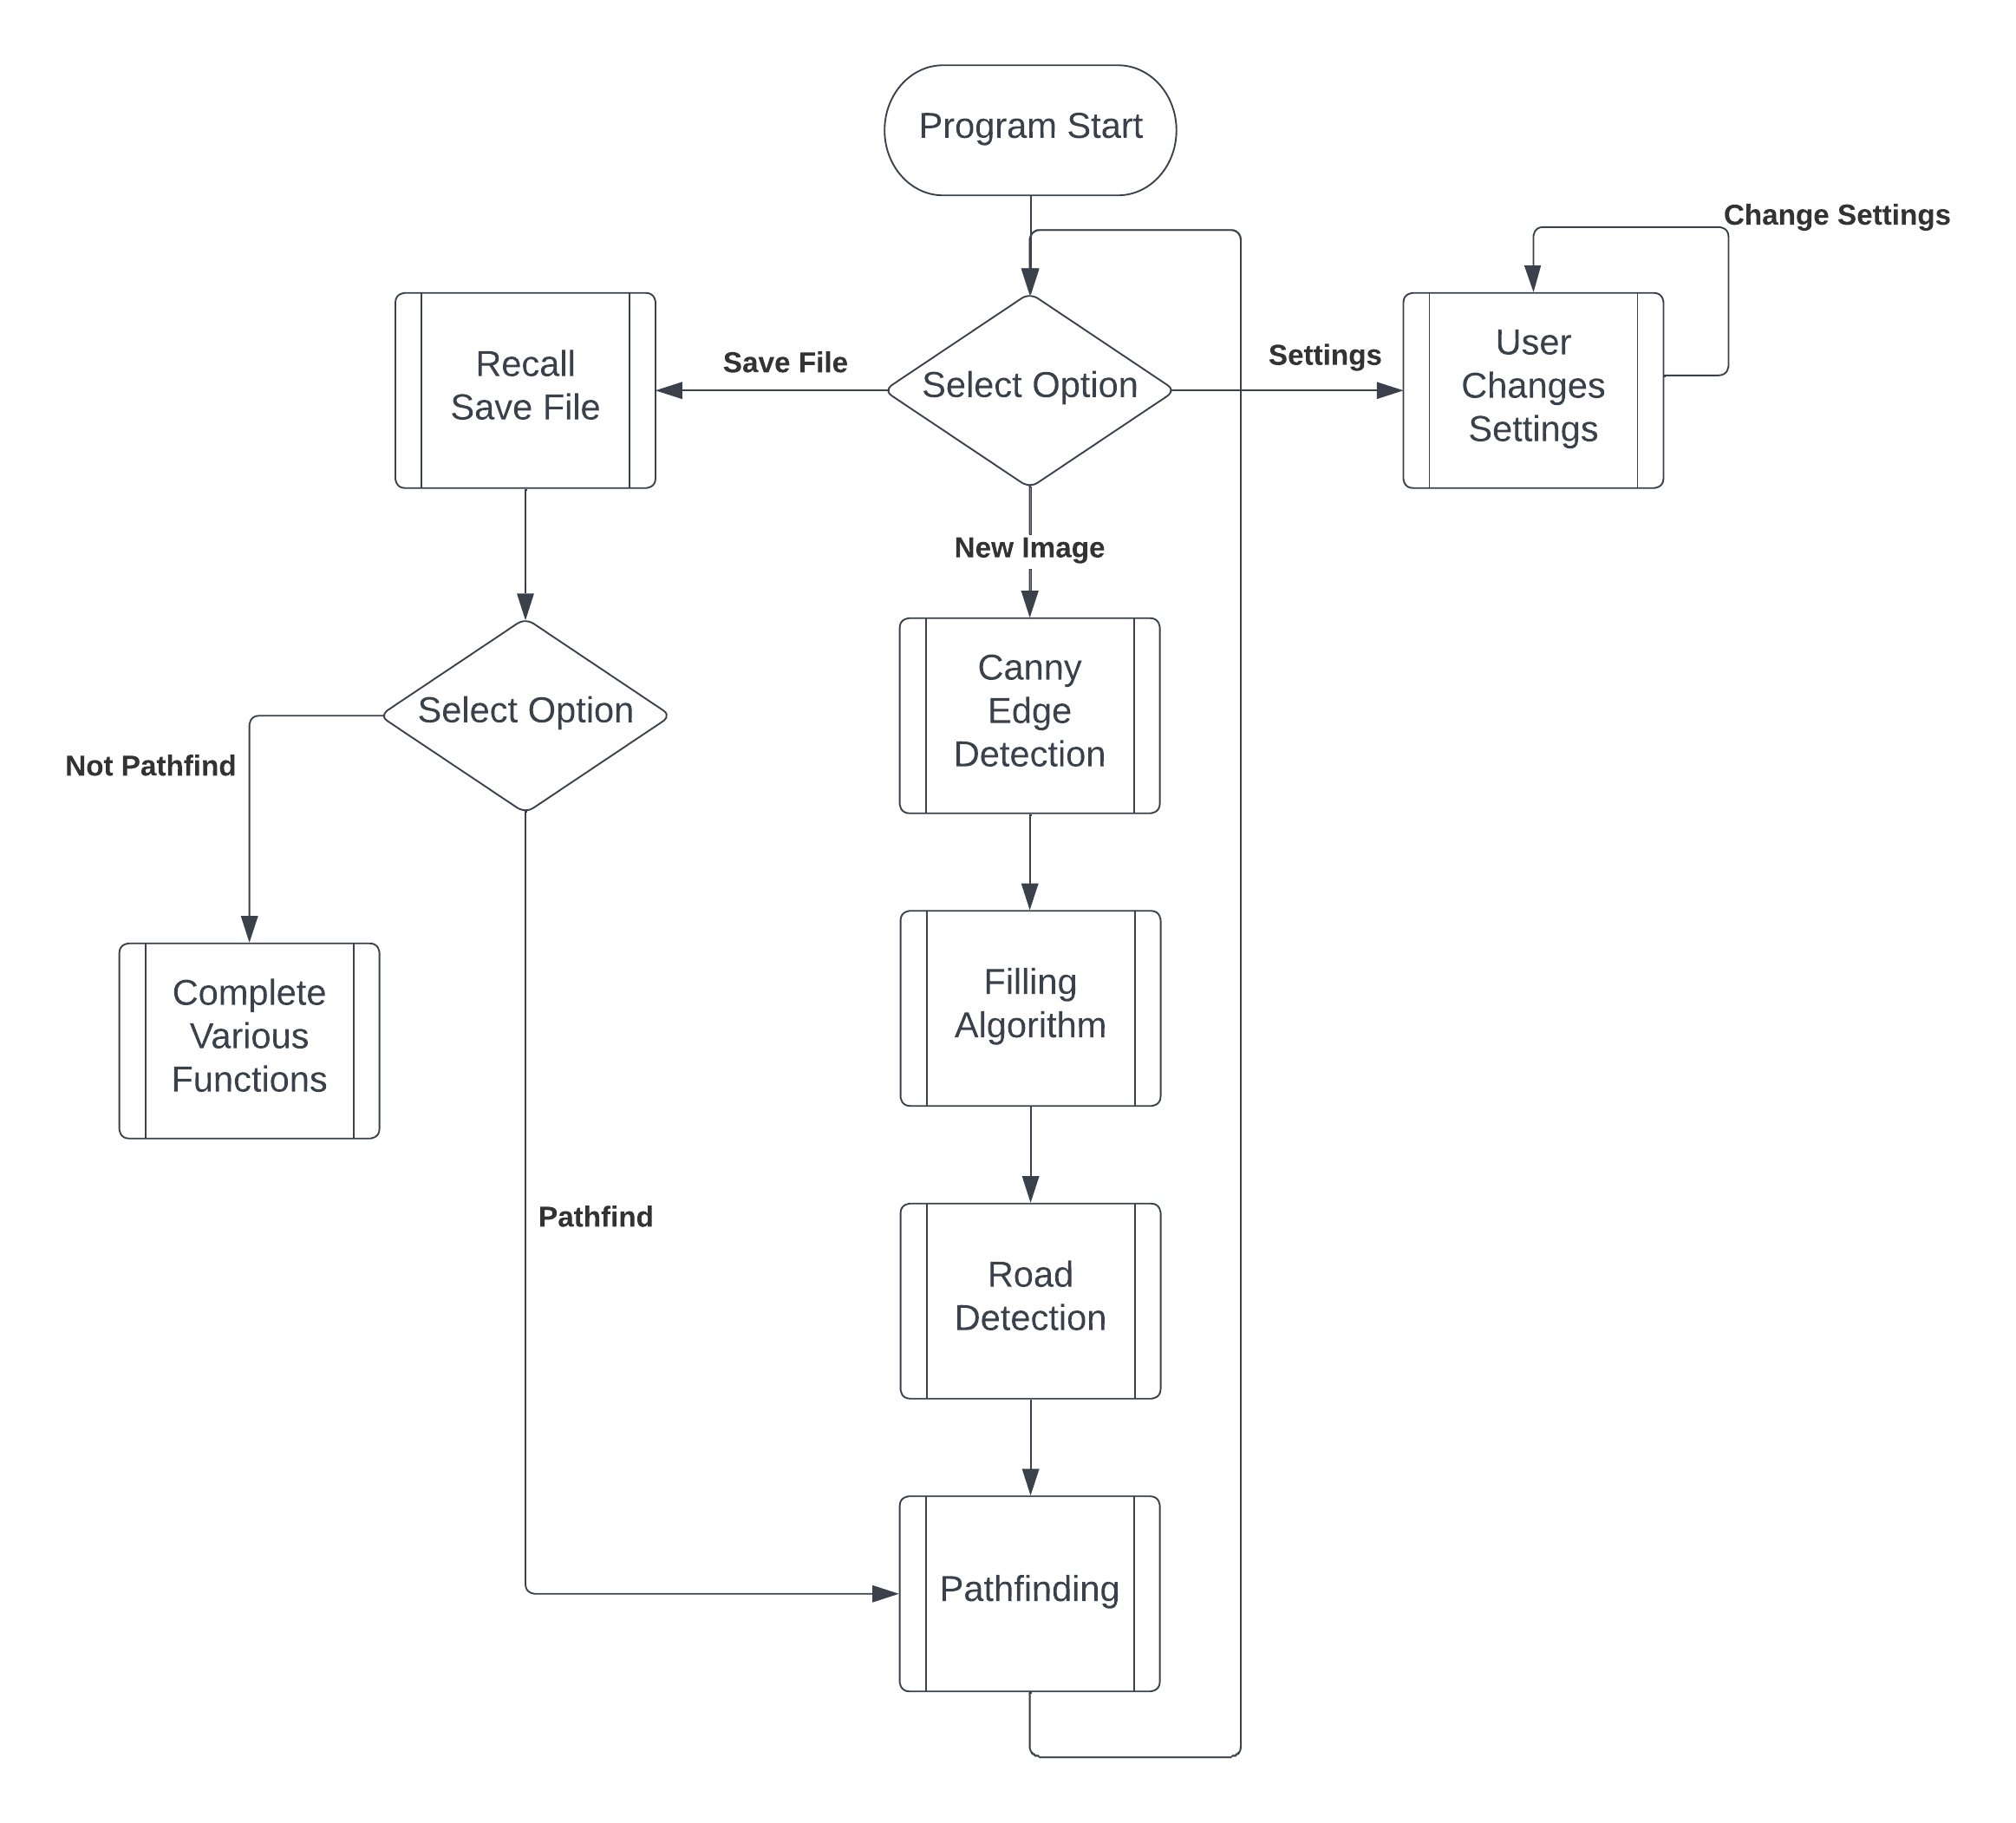
\includegraphics[width=17cm]{images/HighLevelOverview.png}}}
        \caption*{A High Level Overview of the Whole Program}
    \end{figure}

    The version of Edge Detection I will be using as previously stated will be Canny Edge Detection, this is as opposed to Sobel Edge Detection. The main version of filling I will be using is flood fill due to it simple nature to implement ad due to the fact that it does not take much memory and can be made recursive so it performs well. The final main algorithm I will need to use is image kernels and convolution, this will allow me to manipulate the inputted image.

    \subsubsection{Bitmap}
    In order for my program to function a required part of it is that it is able to take an image as an input. In native C# there is no set way to do this. Therefore I needed to use the Microsoft System.Drawing Namespace. This namespace provides access to GDI+ basic graphics functionality. This does limit this project as is to only working on Windows since the library requires access to the GDI+ native library which is only on windows services. \\
    
    The only part of this library I will be using is the Bitmap class. This will allow me to accept all types of images without the need of parsing them myself since this is not the aim of my project. 
    \\ \bk 


\end{flushleft}

    \begin{flushleft}
    \section{Program Testing}
    \subsection{Testing Tables}
    \subsubsection{Targeted Testing Areas}

    \normalsize
    In order to ensure that my NEA conforms to my objectives this following section will test each of them one at a time. As well as this I will test to make sure that each part of the final solution works together and produces the desired and expected output. \\
    An overview of the sections I will test are:
    \begin{enumerate}
        \item User Map Inputs and Subsequent Outputs
        \begin{enumerate}
            \item Loading In Image Files
            \item Creating The Save File
            \item Options Given To User
            \item Conversion To Graph
            \item Error Handling 
        \end{enumerate}\bk
        \item Canny Edge Detection Operations
        \begin{enumerate}
            \item User Variables
            \item Constructor Arguments
            \item Full Flow Thorough
            \item Individual Method Calls
            \item Exceptions
        \end{enumerate}\bk
        \item Road Detection
        \begin{enumerate}
            \item User Variables
            \item Constructor Arguments
            \item Full Flow Through
            \item Individual Method Calls
            \item Exceptions
        \end{enumerate}\bk
        \item Graph Traversal
        \begin{enumerate}
            \item Different Node Placements
            \item Different Algorithms
            \item Other Graph Settings
        \end{enumerate}\bk
        \item Logging and Saves
        \begin{enumerate}
            \item Validity Of Save Files
            \item Contents of Log Files
            \item Save Settings
        \end{enumerate}\bk
        \item Miscellaneous Items + GUI
        \begin{enumerate}
            \item GUI Elements
            \item Matrix Functions
            \item Extensions and Utilities 
            \item Structures
        \end{enumerate}
    \end{enumerate}
    \bk

    It should be noted that in the following tests do not explicitly test objective 5 however it can be seen through out the that this objective has been met. From the icon being clear to the user interface clearing. I believe this combined and the constant evidence shown through the allows me to come to the conclusion that objective 5 has been met.

    \bk
    \setlength\LTpre{0pt}
    \pagebreak
    \subsubsection{User Inputs and Outputs Testing Table}
    \bk
    \normalsize
    \begin{longtable}{| C{0.6cm} | C{2.5cm} | C{4.75cm} | C{4.75cm} | L{1cm} | L{1.4cm} |}
    \hline
    {\footnotesize Test No.}  & Name & Input Data / Description & Expected Output & Pass Fail & Test Evidence \\
    \hline\hline
    \multicolumn{6}{| l |}{\textbf{1.1.(2)} The program should be able to parse a map from a file including...} \\
    \hline
    \rn  & Entering a JPG & Enter the test image as a JPG into the "New Image" promp. & The program should accept the image and be able to process it and show it to the user in the "Preview Form" & Pass & 0:10 \\
    \hline
    \rn  & Entering a PNG & Enter the test image as a PNG into the "New Image" promp. & The program should accept the image and be able to process it and show it to the user in the "Preview Form" & Pass & 0:23 \\
    \hline
    \rn  & Entering a BMP & Enter the test image as a BMP into the "New Image" promp. & The program should accept the image and be able to process it and show it to the user in the "Preview Form" & Pass & 0:33 \\
    \hline
    \rn  & Entering a TIFF & Enter the test image as a TIFF into the "New Image" promp & The program should accept the image and be able to process it and show it to the user in the "Preview Form" & Pass & 0:46 \\
    \hline  
    \multicolumn{6}{| l |}{\textbf{1.1.1} A photograph of an map} \\
    \hline
    \rn  & Entering a Photograph & Enter a photograph into the "new image prompt" & The program should accept the image and be able to process it and show it to the user in the "Preview Form" & Pass & 0:54 \\
    \hline    
    \multicolumn{6}{| l |}{\textbf{1.1.3} A hand drawing of suitable quality (if it is not a message should be shown)} \\
    \hline
    \rn  & Entering a Hand Drawing & Enter a hand drawing into the "new image prompt" & The program should accept the image and be able to process it and show it to the user in the "Preview Form" & Pass & 1:05 \\
    \hline    
    \multicolumn{6}{| l |}{\textbf{1.4} A hand drawing of suitable quality (if it is not a message should be shown)} \\
    \hline
    \rn  & Entering a Small Image (less than 200x200) & Resize test image to be less than 200x200 and then input that into the "New Image" prompt & The program should reject the image and instruct the user as to how to fix the issue. & Pass & 1:17 \\
    \hline
    \rn  & Entering an Invalid Image Path & At the "New Image" prompt an invalid file path should be entered. This test should be repeated with different invalid paths to make sure that all cases are accounted for. & The program should reject all of these inputs without crashing. & Pass & 1:35 \\
    \hline  
    \rn  & Entering an Local Path & The test described described here would consist of a path in the form "../../image.png" for example. & The program should be able to process this path and show the image to the user in the "Preview Image" form. & Pass & 1:52 \\
    \hline
    \rn  & Entering a Valid Save Path & A valid save file path should be entered, use the test image save "save.vmap". & the program should accept this input and show the "Recalled Image" options. & Pass & 12:16 \\
    \hline
    \rn  & Entering an Invalid Save Path & An invalid save file path should be entered. This can be any path ending with "/<something>.vmap" & The program should error and instruct the user how to fix the issue. & Pass & 13:05 \\   
    \hline
    \rn  & Try to Escape Bounds of Option Selector & When in the main menu attempt to go out of bounds of the menu and then select a non existent element. & The option function should not allow the user to go out of the options presented. & Pass & 2:11 \\
    \hline
    \rn  & Try to Break inputs through pre-clicking enter. & When going through menus repeatable click the enter key in order to attempt to get the program to error. This can include clicking misc keys as well as enter. & The program should handle all of these inputs before it then waits for non spammed inputs. It should not error. & Pass & 2:11 \\
    \hline
    \rn  & Remove Characters from Input & When a text input is required, for example the new image prompt when a path is entered, there is a chance that the user could have entered a mistake. Enter random characters then click "Backspace" to remove characters. & The characters should be removed and no error should occur if the backspace is clicked when the carat is at the end it should not error, & Pass & 2:33 \\
    \hline
    
    \multicolumn{6}{| l |}{\textbf{1.3} The inputted map should be converted into a graphs} \\
    \hline
    \rn  & Graph Constructor & Inside the testing menu run the test "Manual Graph", this should generate a predefined graph which contains the nodes and connections as follows. & \begin{enumerate}[label=\Alph*:]
        \item D
        \item F, C
        \item B
        \item A, E, G
        \item D, H
        \item B, G
        \item D, F
        \item E
    \end{enumerate} & Pass & 14:23 \\
    \hline

    \rn  & ToGraph Method & On a small test image the function extension .ToGraph should be run. & The outputted graph should contain the following nodes, {(0,2), (1,2), (2,0), (2,1), (2,2), (2,3), (2,4), (2,5), (3,2), (4,2), (5,2)} & Pass & 14:23  \\
    \hline
    
    \end{longtable}
    \BK

    \pagebreak
    \setcounter{magicrownumbers}{0}
    \subsubsection{Canny Edge Detection Testing Table}
    \bk
    \normalsize
    \begin{longtable}{| C{0.6cm} | C{2.5cm} | C{4.75cm} | C{4.75cm} | L{1cm} | L{1.4cm} |}
    \hline
    {\footnotesize Test No.}  & Name & Input Data / Description & Expected Output & Pass Fail & Test Evidence \\
    \hline\hline 
    \multicolumn{6}{| l |}{\textbf{2.1} At each stage of the edge detection an image should be produced} \\
    \hline
    \rn  & Canny Edge Detect Save Images & Run through a full map detection and at the prompt when it asks if the user would like to save an image at each stage of the Canny edge detection select yes then run the Canny edge detection. & Each stage of the edge detection will have an image saved in the runs/<id> folder. & Pass & 2:58 \\
    \hline
    \multicolumn{6}{| l |}{\textbf{2.3.1} There should be presets to allow quicker processing} \\
    \hline
    \rn & Run A Preset & The test image should be input at the "New Image" prompt. When it comes to picking how the edges should be picked the preset "Screenshot" should be selected. & The program should perform Canny Edge Detection without prompting the user for variables. It should return to user control at the "Invert Image" stage. & Pass & 3:03 \\
    \hline
    \multicolumn{6}{| l |}{\textbf{2.3} The edge detection must have the option to be multi threaded.} \\
    \hline
    \rn  & Cancel A Run & As above the test image should be entered. Both when it comes to the edge picking "Multi-threaded" then entering values then when the program confirms to continue select "No", and when the image is first read selecting "No" when the "Correct Image" prompt shows. & The program should stop running the current image and error with the reason "You asked for the processing of your map to stop." Then it should return to the main menu. & Pass & 3:49 \\
    \hline
    \multicolumn{6}{| l |}{\textbf{2.2} Between each stage the user should be able to repeat} \\
    \multicolumn{6}{| l |}{the last step in order to change parameters.} \\
    \hline
    \rn  & Enter Invalid Values & During the selection of Canny edge detection variations "Multi-threaded" should be chosen. When the program prompts for user inputs a variety of invalid ones should be provided. For example "test", "999999", "1s", "newline", "zero" etc... & The program should check to see if these inputs are within the bounds of the required variables and if they are not it will assume a default value and inform the user. & Pass & 3:16 \\
    \hline
    \rn  & Enter Valid Values & Same prompt as above, in the multi-threaded Canny edge detection variables. However this time valid values should be input, these should test the bounds of the inputs as prompted by the program. & The program should accept these changed values and notify the user of what they have changed too. & Pass & 3:10 \\
    \hline
    \end{longtable}

    
    \textit{The following tests ending in "method" are run one at a time during the slow, single threaded version of Canny edge detection with the exception of the Gradient calculation with error, these are used to test that each stage of the Canny edge detection algorithm are correct and functioning correctly. A full slow run is included afterwards to show that all of the methods work together. The test image is taken from wikipedia. } \\ \bk
 
    \begin{figure}[H]
        \centering
        \subfloat[\centering Example Image Used]{{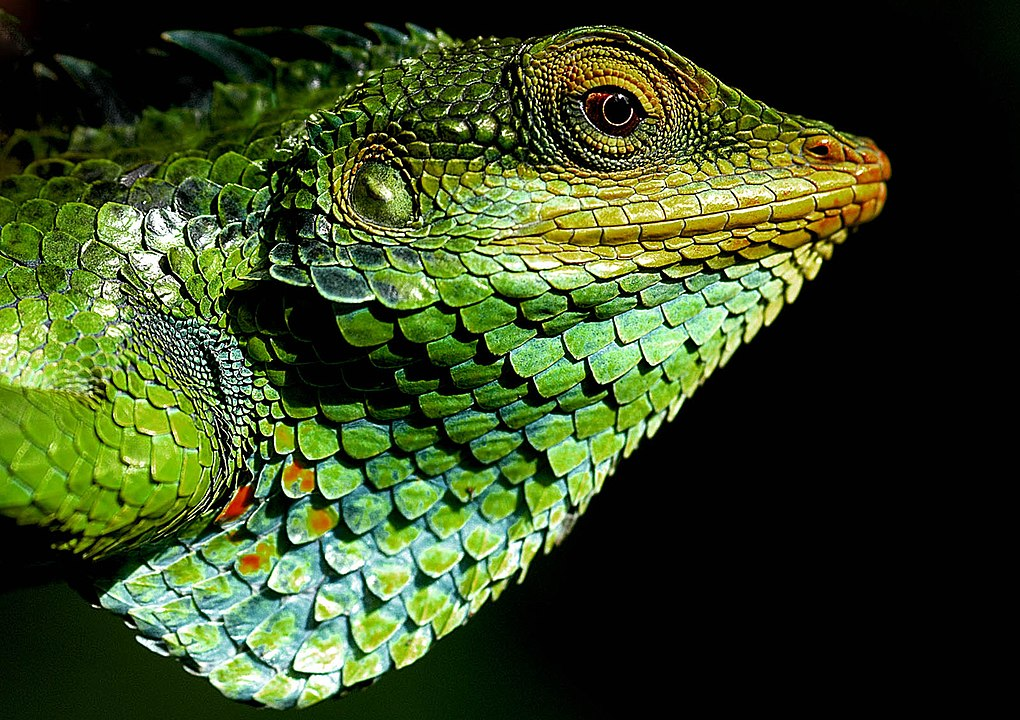
\includegraphics[width=7.5cm]{images/cannyTestImage.jpg}}}
        \caption*{
            \centering Sourced from Wikipedia\textsuperscript{\tiny\textcopyright} \\ \url{https://en.wikipedia.org/wiki/Canny_edge_detector##Walkthrough_of_the_algorithm}
        }
    \end{figure}

    \bk   

    \begin{longtable}{| C{0.6cm} | C{2.5cm} | C{4.75cm} | C{4.75cm} | L{1cm} | L{1.4cm} |}
    \hline
    \multicolumn{6}{| l |}{\textbf{2.4} The edge detection must have the option to be single threaded} \\
    \hline
    \multicolumn{6}{| l |}{\textbf{2.2.1 - 2.2.7} Stages of edge detection.} \\
    \hline
    \rn  & Black and White Method & Canny Edge Detection method should be ran with the original testing image. & \mbox{}{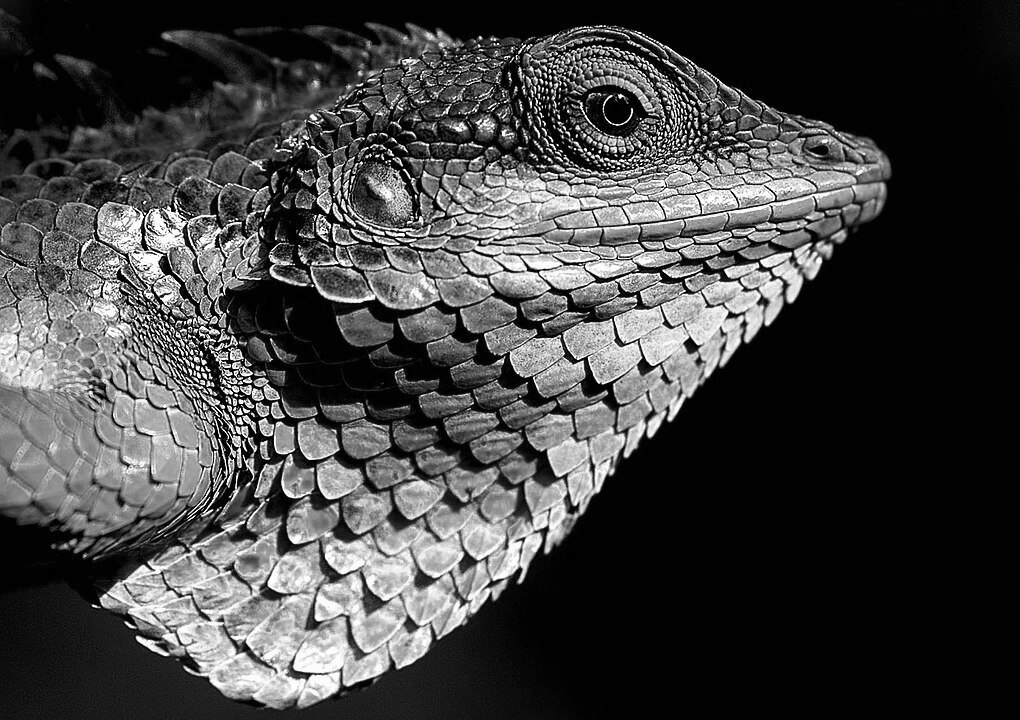
\includegraphics[width=4.5cm]{images/cannyTesting/Canny_Walkthrough_0_Black_White_Filter.jpg }} & Pass & 3:59 \\
    \hline
    \rn  & Gaussian Filter Method & Canny Edge Detection method should be run with the output of the previous step, Black and White conversion. & \mbox{}{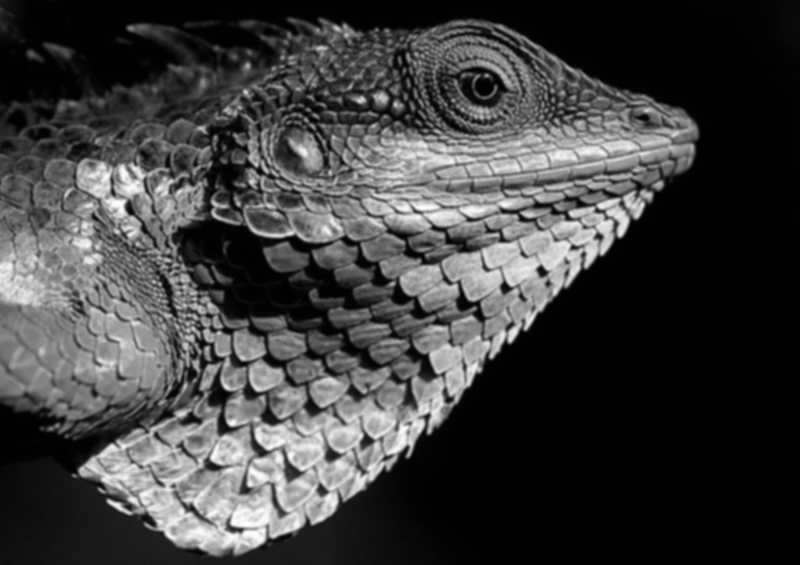
\includegraphics[width=4.5cm]{images/cannyTesting/Canny_Walkthrough_1_Gaussian_Blur.png }} & Pass &  4:10 \\
    \hline
    \rn  & Gradient Calculation Method(s) & This test describes a series of method calls which will all combine to form the image to the right. During this test, the outputs of each individual method call should be shown. The input into the initial methods should be the output from the Gaussian filter.  & \mbox{}{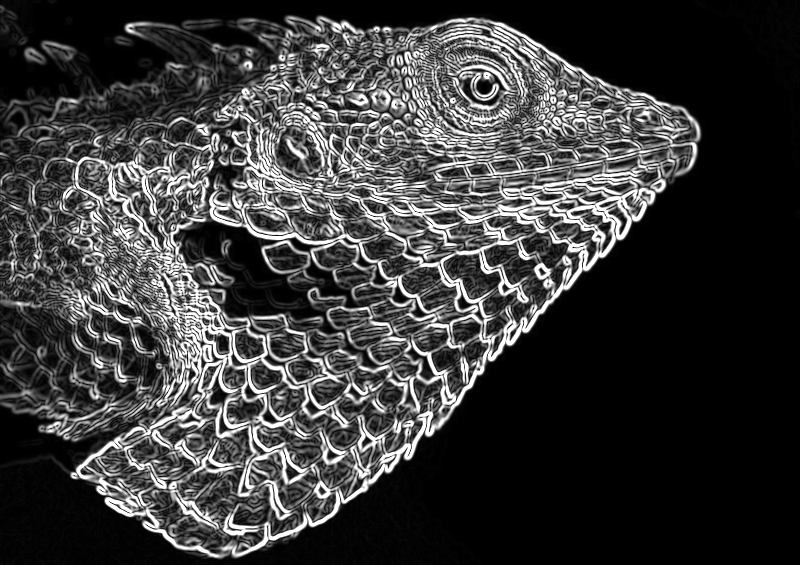
\includegraphics[width=4.5cm]{images/cannyTesting/Canny_Walkthrough_2_Intensity_Gradient.png }} & Pass & 4:23 \\
    \hline
    \rn  & Gradient Calculation Method & This test describes a series of method calls, the initial calls should be run with the output from the Gaussian filter. & The program should not start the gradient calculations, it should not run any further and should throw an ArgumentException. & Pass & 4:23  \\
    \hline
    \rn  & Threshold Method(s) & Canny Edge Detection method should be run with the output of the previous successful step, the non-error gradient calculations. & \mbox{}{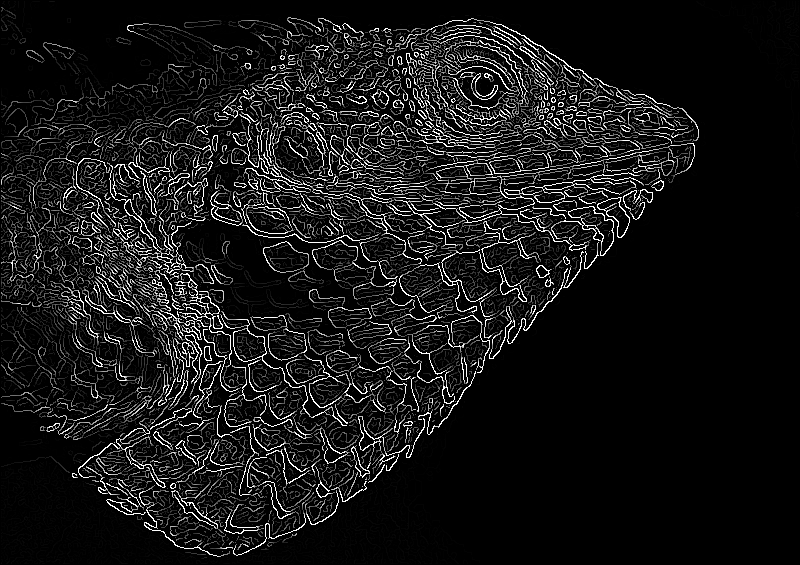
\includegraphics[width=4.5cm]{images/cannyTesting/Canny_Walkthrough_3_Non-maximum_suppression.png }} & Pass & 4:30 \\
    \hline
    \rn  & Hysteresis Method & Canny Edge Detection method should be run with the output of the previous step, the gradient calculation methods. After this test the image will be in its final edge detected form. & \mbox{}{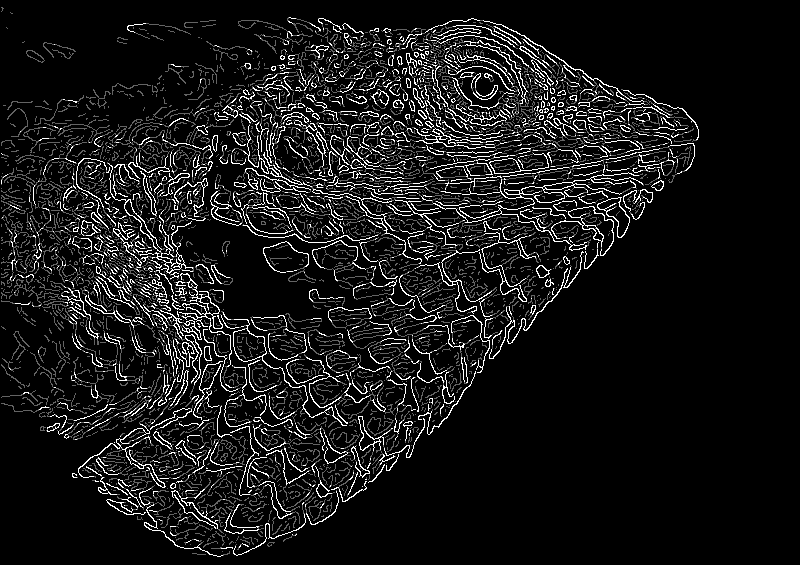
\includegraphics[width=4.5cm]{images/cannyTesting/Canny_Walkthrough_4_Double_Threshold.png }} & Pass & 4:38 \\
    \hline
    \rn  & Run Full Custom Run (Quick) & Using the "RunQuadrant" method in order to quickly process an image. The default values should be used and the result file should be compared to the image to the right. & \mbox{}{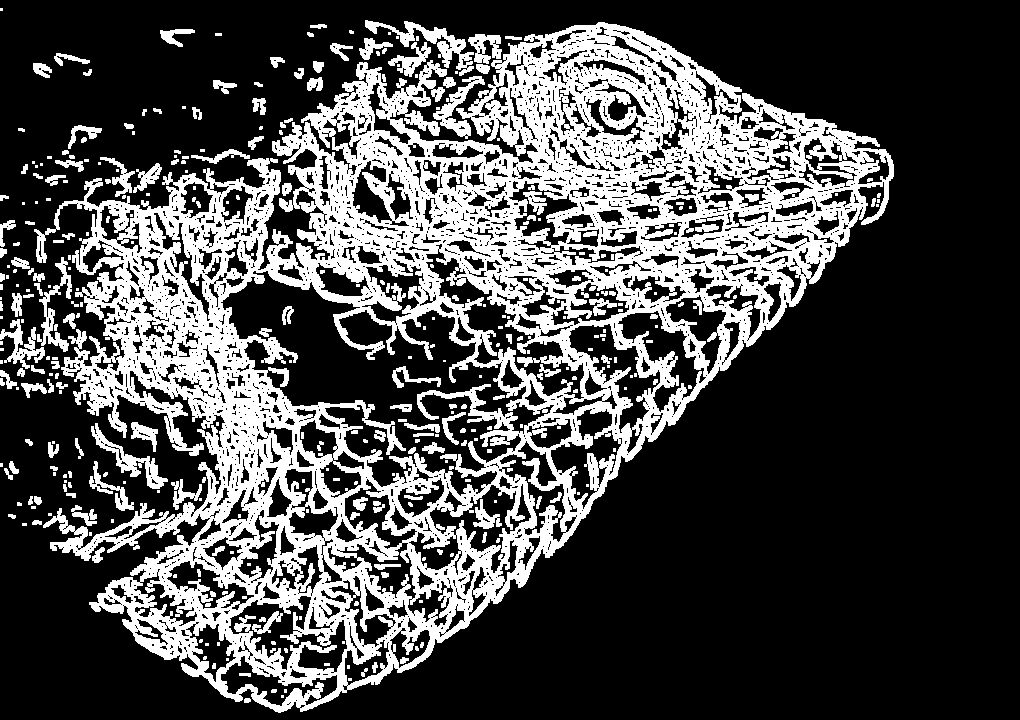
\includegraphics[width=4.5cm]{images/cannyTesting/Canny_Walkthrough_5_Hysteresis.png }} & Pass & 11:15 \\
    \hline
    \rn  & Run Full Custom Run (Slow) & The slow single threaded version should be used, this should allow the user to change and go back on variables if they do not like the output. The final expected result is seen to the left. At each stage however the processed images should be shown. & \mbox{}{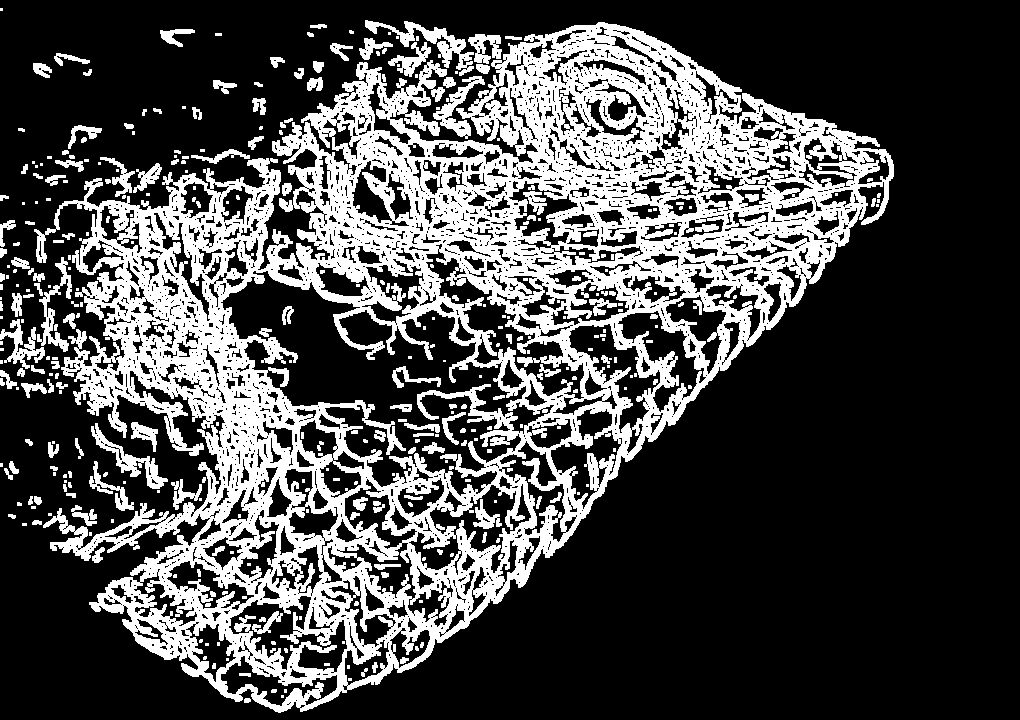
\includegraphics[width=4.5cm]{images/cannyTesting/Canny_Walkthrough_5_Hysteresis.png }} & Pass & 3:57 \\
    \hline
    \end{longtable}
    \BK
    \pagebreak
    \setcounter{magicrownumbers}{0}
    \subsubsection{Road Detection and Graph Conversion Testing Table}
    \bk
    \normalsize
    \begin{longtable}{| C{0.6cm} | C{2.5cm} | C{4.75cm} | C{4.75cm} | L{1cm} | L{1.4cm} |}
    \hline
    {\footnotesize Test No.}  & Name & Input Data / Description & Expected Output & Pass Fail & Test Evidence \\
    \hline\hline
    \multicolumn{6}{| l |}{\textbf{3} The Program must overlay the detected roads onto the original imaged} \\
    \multicolumn{6}{| l |}{\textbf{3.2.4 - 3.2.5} The total filled image can be displayed to the user} \\
    \hline
    \rn  & Full Run of Road Detection & Using the test image, after the run of Canny edge detection the result should not be inverted and the road threshold should be set to 0.3 and then the road detection run. & \mbox{}{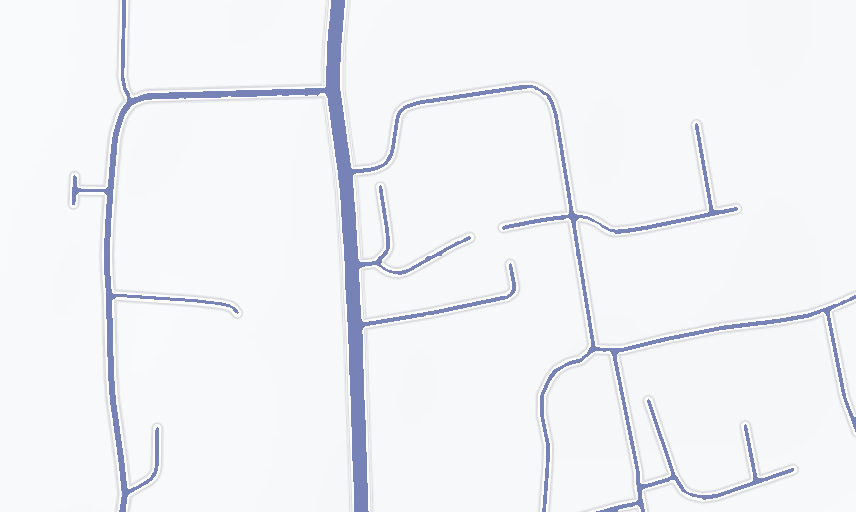
\includegraphics[width=4.5cm]{images/roadExamples/comb.png }} & Pass & 5:06 \\
    \hline
    \multicolumn{6}{| l |}{\textbf{3.2.3} The percentage threshold for non roads much be changeable by the user } \\
    \hline
    \rn  & Enter Valid Threshold & When the road prompt is shown a number within the shown range should be entered. & The program should accept this new input and use it in the following process. It should also clearly show the user that the value has been changed. & Pass & 4:54 \\
    \hline
    \rn  & Enter Invalid Threshold & When the road prompt is shown a number out the shown range should be entered as well as this invalid strings should be entered. Examples include "test", "ds@13=kle3q" etc... & The program should use the default value and not error. It should clearly show the user that the default value has been used. & Pass & 5:05 \\
    \hline
    \rn  & Redo Threshold & After the road detection has been performed the user is prompted whether the result is as they like, at this prompt "No" should be entered. & The program should exit with an error message "You asked for the processing of your map to stop.". It should then return to the main menu. & Pass & 5:00 \\
    \hline
    \multicolumn{6}{| l |}{\textbf{3.2.1} The image should have the option to be inverted} \\
    \hline
    \rn  & Invert Image Method & An all black image 100x100 image should be fed into this method and then the output should be a 100x100 white square. & \mbox{}{
\includegraphics[width=4.5cm]{images/roadExamples/white.png }} & Pass & 4:52 \\
    \hline
    \multicolumn{6}{| l |}{\textbf{3.2.2} A filling algorithm should be applied to the image} \\
    \hline
    \rn  & Fill Image Method & An image with 4 white quadrants should be fed into the function. This image should be 200x200. The colours used are pseudo randomly generated so they may not be identical to the expected output, the 4 quadrants should still be filled however. & \mbox{}{
\includegraphics[width=4.5cm]{images/roadExamples/quadsFilledExample.png }} & Pass & 5:00 \\
    \hline
    
    \end{longtable}
    \BK
    \pagebreak
    \setcounter{magicrownumbers}{0}
    \subsubsection{Graph Traversal Testing Table}
    \bk
    \normalsize
    \begin{longtable}{| C{0.6cm} | C{2.5cm} | C{4.75cm} | C{4.75cm} | L{1cm} | L{1.4cm} |}
    \hline
    {\footnotesize Test No.}  & Name & Input Data / Description & Expected Output & Pass Fail & Test Evidence \\
    \hline
    \end{longtable}
    \textit{The following are all performed on the test image unless otherwise stated, some of the tests are conducted separate to the main program but still using the same methods and functions. This is due to the fact that some of these traversal algorithms are never shown to the user.} \\
    \bk
    \begin{longtable}{| C{0.6cm} | C{2.5cm} | C{4.75cm} | C{4.75cm} | L{1cm} | L{1.4cm} |}
    \hline
    \multicolumn{6}{| l |}{\textbf{4.1.2}  The Program should Implement Searching Algorithms} \\
    \multicolumn{6}{| l |}{ these do not have to be shown to the user.} \\
    \hline
    \multicolumn{6}{| l |}{\textbf{4.1.2.2}  This includes DFS (Depth-first search).} \\
    \hline
    \rn  & Run DFS & Using the test image run depth first search. Since this test is not shown the user use the premed video. & To the human eye it should look like the path is going "down" more than it is going across, in essence it should look like the image is "filling up". & Pass & 5:25 \\
    \hline
    \multicolumn{6}{| l |}{\textbf{4.1.2.1}  This includes BFS (Breadth-first search).} \\
    \hline
    \rn  & Run BFS Location 1 & Using the test image run breadth first search. Since this test is not shown the user use the premed video. & To the human eye it should look like the path is going "across" more than it is going down, in essence it should look like something is spreading from a single point source out to the rest of the image. & Pass & 5:47 \\
    \hline
    \rn  & Run BFS Location 2 & Using the test image run breadth first search. Since this test is not shown the user use the premed video. & To the human eye it should look like the path is going "across" more than it is going down, in essence it should look like something is spreading from a single point source out to the rest of the image. & Pass & 6:10 \\
    \hline
    \multicolumn{6}{| l |}{\textbf{4.1.1}  The Program should implement Routing Algorithms} \\
    \hline
    \multicolumn{6}{| l |}{\textbf{4.1.1.1}  This includes Dijkstra’s algorithm.}
    \\
    \hline
    \rn  & Run Dijkstra & Using the save.vmap perform graph traversal using the algorithm "Dijkstra's" setting the start node and end node anywhere on the graph then clicking "Pathfind" & The program should perform Dijkstra's algorithm on the image before drawing the path which it found as the most optimal route. & Pass & 6:35 \\
    \hline
    \rn  & Run Dijkstra Same Start Different End & Using the same start node as the previous test the end node should be moved, then "pathfind" should be clicked & The program should instantly draw the new path without having to re-perform Dijkstra's & Pass & 6:55 \\
    \hline
    \rn  & Run Dijkstra Different Start Same End & With the same end node as above, the start node should be moved to another point on the image then the "Pathfind" button should be clicked. & The program should perform Dijkstra's again due to the start node being moved. & Pass & 7:27 \\
    \hline
    \rn  & Run Dijkstra Different Start Different End & Move both the start and end nodes from the ones above and then click "Pathfind" & As above the program will have to recalculate the entire path since the start node has moved. & Pass & 7:04 \\
    \hline
    \rn  & Run Dijkstra End on Find & Enable the setting "endOnFind" and then perform Dijkstra's on two nodes which are relatively spatially close to each other. Then click "Pathfind". & The program will perform Dijkstra's however if it locates the end node it will pause pathfinding there and stop. It should be faster than regular Dijkstra's & Pass & 7:54 \\
    \hline
    \multicolumn{6}{| l |}{\textbf{4.1.1.2}  This includes A* (a specialised Dijkstra)}
    \\
    \hline
    \rn  & Run A* Image & Two nodes should be placed on points on the graph, then the "Pathfind" button should be clicked. & The algorithm will run the A* algorithm which using a heuristic algorithm will more efficiently find a path to the end node. It should run faster than Dijkstra's. & Pass & 8:05 \\
    \hline
    \end{longtable}
    \BK

    \pagebreak
    \setcounter{magicrownumbers}{0}
    \subsubsection{Logging and Saves Testing Table}
    \bk
    \normalsize
    \begin{longtable}{| C{0.6cm} | C{2.5cm} | C{4.75cm} | C{4.75cm} | L{1cm} | L{1.4cm} |}
    \hline
    {\footnotesize Test No.} & Name & Input Data / Description & Expected Output & Pass Fail & Test Evidence \\
    \hline\hline
    \multicolumn{6}{| l |}{\textbf{8} The program should have re-callable settings} \\
    \hline
    \rn  & Read Normal Settings File & Start the program and navigate to "Settings" & No error should occur and settings should be able to be changed. & Pass & 8:27 \\
    \hline   
    \rn  & Read Corrupt Settings File & Remove and rename sections of settings file. Then as above. & The program should error and instruct the user how to correct the fault. & Pass & 8:47 \\ 
    \hline
    \rn  & Programmatically Alter Normal Settings File & Navigate to "Settings" and change settings in each sub menu and show altered settings.conf & settings.conf should show the changed settings. Before and after should be shown side by side. & Pass & 8:35, 9:14 \\
    \hline
    \rn  & Programmatically Alter Corrupt Settings File & Remove entry from settings then attempt to alter settings similar to above. & The program should error and instruct the user how to correct the fault. & Pass & 8:47 \\
    \hline
    \rn  & Save Corrupt Settings File & Attempt to enter the settings menu, alter a setting and the exit. Upon the "exit" condition the file will be saved. & The program should not let the user alter the settings and should error and instruct the user how to proceed. & Pass & 8:47 \\
    \hline
    \rn  & Save Normal Settings File & Enter the settings menu, alter a setting and then exit. Upon the "exit" condition the file will be saved. & The file should save without issue and a side by side of the programmatically altered file should be shown. & Pass & 8:44 \\
    \hline
    \rn  & Manually Alter Settings File & Open the settings.conf file and change settings values then save and restart the program. Once the program has been restarted check the settings in the menu to see if they have been changed. & The changed settings state should be mirrored in the settings menu. & Pass & 9:24 \\
    \hline
    \multicolumn{6}{| l |}{\textbf{9 / 10}  The program settings / save files should be easily movable. } \\
    \hline
    \rn  & Run Program Fresh & Run the executable of the program. & In the file directory 3 folders should be created. Runs, Saves, Logs. And inside of the log file there should be a file called master.txt Inside the master log a startup message should be recorded. There should also be a config file created. & Pass & 10:00 \\
    \hline
    \rn  & Re-run Program & Close the program which was just started. Then run the executable. & No files should be created or deleted however there should be a new entry in the master.log & Pass & 10:07 \\
    \hline
    \rn  & Delete Some Folders and Re-run & In the directory where the program file is contained the programmatically created folders should be deleted. Not all but some. & When the program is restarted the files should be recreated & Pass & 10:10 \\
    \hline
    \rn  & Full Run and Check Master Log & After the previous tests have been completed (ones involving a raw image being processed) the master.log should be checked & when checking the master log there should be a message saying that a run has started and that it ends. Furthermore it should contain the ID of the run. & Pass & 10:19 \\
    \hline
    \rn  & Full Run and Check Individual Log & After the previous tests have been completed (ones involving a raw image being processed) the individual unique run log should be checked & Inside the per run log there should be each step of the edge detection and others depending on pathfinding. & Pass & 11:08 \\
    \hline
    \rn  & Cause Error and Check Log & Check the log after one of the input validation tests. & There should be a line in the master file referencing the error. & Pass & 11:23 \\
    \hline
    \multicolumn{6}{| l |}{\textbf{7.1} The map in a binary file format } \\
    \hline
    \multicolumn{6}{| l |}{\textbf{7.2} The saved images from the processing of the map should be able to be saved in a  } \\
    \multicolumn{6}{| l |}{ compressed format. } \\
    \hline
    \rn  & Full Run with Save To Zip & Process a whole image asking for it to be saved. The setting "zipOnComplete" enabled. This will ensure that after the processing the file is saved. & After the run has completed in the root directory a zip file will be created containing any partial images, save file and logs. & Pass & 11:18 \\
    \hline
    \rn  & Run with Detailed Logging & Enable the setting "detailedLogging" and run through a full process of map recognition. & To the side of the main screen during the process detailed log messages of what exactly is going on should be shown. & Pass & 11:18 \\
    \hline
    \rn  & View Save File From Program & Using the test image save attempt to read it into the program. & The program should accept the test image save and take the user to the save image file. & Pass & 12:16 \\
    \hline
    \multicolumn{6}{| l |}{\textbf{7.6} The saved binary file should be able to be have its description changed } \\
    \hline
    \rn  & Change Save File Information & First the file information should be viewed by selecting "View File Information" then once what you know what you wish to change the "Change File Information". Then any of the details may be changed. & Once a change has been made the program should create a copy of the save file with the new info contained within and the rest of the old data. & Pass & 13:21 \\
    \hline
    \multicolumn{6}{| l |}{\textbf{7.3} The saved binary file should be able to be cloned } \\
    \hline
    \rn  & Clone Save File & On the save file info page select "Clone" & The program should create a copy of the save file with all of its details exactly the same. & Pass & 12:25 \\
    \hline
    \multicolumn{6}{| l |}{\textbf{7.5} The saved binary file should be able to be renamed } \\
    \hline
    \rn  & Rename Save File & In the save file menu, "Rename" should be selected. A new name should be entered. & The program will be renamed to the value which the user entered. & Pass & 12:36 \\
    \hline
    \multicolumn{6}{| l |}{\textbf{7.7} The saved binary file should be able to be able to be deleted } \\
\hline
    \rn  & Delete Save File & As above select "Delete" and then follow the prompts to delete the file. & Once the user has navigated to the confirm button the program will delete the save file. & Pass & 12:51 \\
    \hline
    \rn  & Recall to Pathfind Save File & In the recalled options select the pathfind option. & When this option is selected the program will turn over to the pathfinding image form. From there the user can perform graph traversal on it. & Pass & 13:09 \\
    \hline
    \end{longtable}
    \BK

    \pagebreak
    \setcounter{magicrownumbers}{0}
    \subsubsection{Miscellaneous Testing Table}
    \bk
    \normalsize
    \begin{longtable}{| C{2cm} | L{12cm} | C{2cm} |}
    \hline
    {\footnotesize Test No.} & Name & Pass Fail \\
    \hline
    \multicolumn{3}{| c |}{ \normalsize{\textbf{It can be said that since the program works given all tests so far, and that all}} } \\
    \multicolumn{3}{| c |}{ \normalsize{\textbf{the following tests test functionality which is integral to said program, it}} } \\
    \multicolumn{3}{| c |}{ \normalsize{\textbf{can be said that these functions work in the capacity required by the program.}} } \\
    \hline\hline
    \multicolumn{3}{| l |}{ \normalsize{\textbf{6.1}:The program must implement a matrix class } } \\
    \hline
    \rn  & Matrix Constructor & Pass \\
    \hline
    \rn  & Array Index Accessing of Matrix & Pass \\
    \hline
    \rn  & Adding Matrices & Pass \\
    \hline
    \rn  & Subtracting Matrices & Pass \\
    \hline
    \rn  & Matrix Multiplication & Pass \\
    \hline
    \rn  & Scalar Multiplication & Pass \\
    \hline
    \rn  & Matrix Minimisation & Pass \\
    \hline
    \rn  & Matrix Convolution & Pass \\
    \hline
    \multicolumn{3}{| l |}{ \normalsize{\textbf{X.X}: No set objective but contribute to the simplistic and user input objectives} } \\
    \hline
    \rn  & Progress Bar Creation & Pass \\
    \hline
    \rn  & Progress Bar Update Action & Pass \\
    \hline
    \rn  & Coord Struct ToString & Pass \\
    \hline
    \rn  & Coord Struct Equals Method & Pass \\
    \hline
    \rn  & Coord Struct Equals Opperator & Pass \\
    \hline
    \rn  & Coord Struct Not Equals Opperator & Pass \\
    \hline
    \rn  & 2D Double Array ToBitmap Extension & Pass \\
    \hline
    \rn  & Bitmap ToDoubles Extension & Pass \\
    \hline
    \rn  & 2D RGB Structure ToBitmap Extension & Pass \\
    \hline
    \rn  & 2D Doubles ToGraph & Pass \\
    \hline
    \rn  & SetPixel Extension & Pass \\
    \hline
    \rn  & GetPixel Extension & Pass \\
    \hline
    \rn  & Gaussian Distribution Utility & Pass \\
    \hline
    \rn  & Bound Utility & Pass \\
    \hline
    \rn  & TryBound Utility & Pass \\
    \hline
    \rn  & Degree to Radian Utility & Pass \\
    \hline
    \rn  & Radian to Degree Utility & Pass \\
    \hline
    \rn  & Map Radian To Pixel Utility & Pass \\
    \hline
    \rn  & Combine Bitmap Utility & Pass \\
    \hline
    \rn  & Split Image Utility & Pass \\
    \hline
    \rn  & combine Quadrants Utility & Pass \\
    \hline
    \rn  & Inverse Image Utility & Pass \\
    \hline
    \rn  & Generic Rebuild Path Utility & Pass \\
    \hline
    \rn  & Is Yes Utility & Pass \\
    \hline 
    \rn  & Get Red Utility & Pass \\
    \hline
    \rn  & Get Green Utility & Pass \\
    \hline
    \rn  & Get Blue Utility & Pass \\
    \hline
    \rn  & Get Average Utility & Pass \\
    \hline
    \rn  & Get Industry Average Utility & Pass \\
    \hline
    \rn  & Get If Exists Utility & Pass \\
    \hline
    \rn  & Get Distance Between Nodes Utility & Pass \\
    \hline
    \end{longtable}
    \pagebreak
    \textit{The following tests refer to pathfinding through any given map using A-Star, this is testing the "Pathfind Image Form". The test image recalled from a save file will be used for all of these tests unless otherwise specified.} \\ \bk
    \begin{longtable}{| C{0.6cm} | C{2.5cm} | C{4.75cm} | C{4.75cm} | L{1cm} | L{1.4cm} |}
    \hline
    \multicolumn{6}{| l |}{\textbf{5} | The Program must have a Clear and Simplistic GUI.} \\
    \multicolumn{6}{| l |} {\textbf{5} | (The following show that it is easy to use and hard to break the user inputs.)} \\
    \hline
    \rn  & Select No Nodes & Neither left or right mouse buttons should be clicked and then the "Pathfind" button should be clicked. & The program should not run and instantly go back to waiting for input. & Pass & 13:53 \\
    \hline
    \rn  & Select One Node & Only one left or right mouse button should be clicked and then the "Pathfind" button should be clicked. & The program should not run and instantly go back to waiting for input. & Pass & 13:57 \\ 
    \hline
    \rn  & Select Two Nodes & Neither left or right mouse buttons should be clicked and then the "Pathfind" button should be clicked. & The program should run and after some time should then wait for input. & Pass & 14:00 \\
    \hline
    \rn  & Select One Node Off Path & First the "snapToGrid" setting to false. Set one node off the path and one on and then click the "Pathfind" button. & The program should not run and instantly go back to waiting for input. & Pass & 14:08 \\
    \hline
    \rn  & Select Two Nodes Off Path & First the "snapToGrid" setting to false. Set both nodes off the path and then click the "Pathfind" button. & The program should not run and instantly go back to waiting for input. & Pass & 14:23 \\
    \hline
    \rn  & Select One Node Off Path One On with Dijkstras & First the "snapToGrid" setting to false. Set one node off the path and one on and then click the "Pathfind" button. & The program should run momentarily and allow then return to waiting. If the end node is then placed back on the road the pathfinding should be instant. & Pass & 14:33 \\
    \hline
    \rn  & Click Continue Button in View Image Form & Get to a situation where the "View Image" form is shown. This can be during Canny Edge Detection or when a new image is processed. Then click the continue button. & The button should cause the form to close itself and allow the program to continue. & Pass & 14:23  \\
    \hline
    \end{longtable}
    \BK

    \pagebreak
    \subsection{Testing Video}
        Please find below several links to the NEA testing Video: as well as a QR code. The timestamps from the table refer to points in this video. Timestamps are also contained within the description. \\ \bk
        
        \begin{center}
            \quad
            \qrcode{https://youtu.be/cJqFovg27Bo}
            \\ \BK
            \large
            \text{Raw URL: \url{https://youtu.be/cJqFovg27Bo}} \\            
            \normalsizeer
            \textit{charlie JULIET quebec FOXTROT oscar victor golf two seven BRAVO oscar} \\ \bk  
            \large
            \text{Short URL: \url{https://shorturl.at/dT158}} \\
            \normalsizeer
            \textit{delta TANGO one five eight}
        \end{center}        
\end{flushleft}

    % TODO
\begin{flushleft}
    \section{Technical Solution} 

    \subsection{Code Table of Contents}
    

\end{flushleft}

    \begin{flushleft}
    % this is all about reflection on how successful the project has been
    % no real excuse to not get full marks
    % Section on overall effectiveness of the system, what went well what went wrong, be detialed
    % Section on the objcetives, judge how effectivly it has been met also comment on how the solition might be inproved. Can refer back to testing
    % End user feedback, the end user needs to feedback to how effective the solution is. Needs to be a critical evaluation. Has to be critasizms, what needs to be improved, but also what went well. D E T A I L
    % My insight into their feedback is what gets the marks not their feedback on its own.
    % System improvements, explain the outline how you might go about making improvments based on the evaluation and objective completeion and end user feedback. Be honest.
    \section{Evaluation}

    \subsection{Objective Completion}
    \begin{longtable}{| C{2.4cm} | L{12.6cm} |}
        \hline
        \textbf{Objective Number} & \textbf{Completion Details}
        \hline
        1.1 & In its current form my program is able to take an image of a map and convert it successfully into routable data. It accepts most common image formats. \\
        \hline
        1.2 & Should the user select to do so the program will prompt them to enter all of the information about the image that was supplied. Once it collects this information it stores the data in a temporary class in memory and then writes it to a binary save after it has finished processing. \\ 
        \hline 
        1.3 & Once Canny edge detection has been performed upon the image and the set roads have been picked out it, it converts it to a graph inside a windows form to allow the user to pathfind through it. \\
        \hline
        1.4 & When an error occurs the program logs it to a log file allowing the user to go back and see what exactly caused the error. It also shows a large box in the middle of the screen making it clear what just happened. It also contains a small message about how to remedy the error. \\
        \hline
        \hline
        2.1 & Should the user choose to do so the program can save a image of the current edge detection stage. As well as this if the user selects to run a specific way the program will show a preview of the image while it is running.\\
        \hline
        2.2 & Similar to above should the user chose to do so they can have the program pause at every stage and allow them to input different variables and see the effect that this has. \\
        \hline
        2.3 & If the user choses to do so there are 3 presets they can pick from which all they need to do is select then the program will run through all stages autonomously, alternatively they can choose to input values at the very beginning and run from there. \\
        \hline
        2.4 & This is completed should the user select the single threaded option at the Canny edge detection stage. \\
        \hline
        \hline
        3.1 & After the Canny edge detection has finished, a windows form is shown to the user, this contains the output of the edge detection after it has gone through the embossing kernel and pixel filling. \\
        \hline
        3.2 & With the result of the canny edge detection the paths can be detected using a combination of filling and coordinate maths. \\ 
        \hline
        \hline
        4.1 & The user can change the map traversal algorithm in the program settings in order to change the behaviour of the algorithms used, two algorithms are . \\
        \hline
        4.2 & Depending on the algorithm which the user has selected to use, when the program reaches the pathfinding windows form, the details about that specific algorithm are displayed. Examples incudes the complexity and amount of nodes processed. \\
        \hline
        \hline
        5.1 & At the bottom of the user interface there is a small window title telling the user exactly at what stage they are. As well as this the title of the window also updates dynamically depending on which stage the user is at. \\ 
        \hline 
        5.2 & There are only two forms in the final version of my program. The soul purpose of the first form is to display images to the user, it contains nothing but the image itself and a continue button. The second form is used to allows the user to interact with the image and click on points to pathfind from one to another. \\ 
        \hline
        5.3 & In the settings, should the user chose to select it there is the option for logging to be shown to the user as it is generated or to be hidden. \\
        \hline
        5.4 & Every time that the user moves to the next stage there is a screen clear meaning that no data is left behind to clutter up the GUI \\
        \hline
        \hline
        6.1 & In order for the Canny edge detection to work the program must be able to perform matrix operations. The matrix class can perform all of the operations outlined in this objective. \\
        \hline
        6.2 & The program implements the graph class and it is heavily used in the pathfinding image form where it has pathfinding algorithms performed on it. It is seen to work due to paths being able to be drawn on the image. \\
        \hline
        \hline
        7.x & As outlined in all the sub objectives the program should be able to save the map as a binary file. This is seen where if the user choses so a .vmap file will be produced containing all the information related to the pathfinding and processing of said image. There are also options within the program such as deletion and renaming as required by the extension objectives.\\
        \hline
        \hline
        8.x & There is a save file which contains all the information relating to settings inside the program. This file persists over program instances and also can be moved manuals to a new version of the program. As stated in the objectives it contains settings for all the functions listed and more. \\
        \hline
        \hline
        9 & As stated above the settings file is a normal windows file and therefore can be moved manuals or even the text inside it copied to another settings file.\\
        \hline
        \hline
        10 & All save files are stored in a .vmap file which is a custom binary file. This means that they can be emailed, put on a USB or any other method of transporting files.\\
        \hline
        \end{longtable}
    \BK
    \pagebreak


    \subsection{End User Feedback}
    \begin{enumerate}
        \item What do you think about the overall program? \\ \bk
        "
        The overall program is very impressive with the given examples, when it comes down to the core features I would want from a program like this it comes away with all of them. Some things do feel slightly rough around the edges and if this where to be a tool I would recommend it would need ot be a little more modern, perhaps a website. \\ \bk

        From an ease of use stand point I think that this program excels at making it easy for a user to tell where they are in the whole process. The addition of the small page title at the bottom of the screen makes it intuitive and easy to work out whats going on. The addition of user settings is also nice since it allows me to change various aspects of the program without having to be an expert. \\ \bk

        I really like the way in which when there is a visual thing the program seamlessly floats to the front and lets you see the image. The one thing which is not amazing about it is that by default it forces itself to the front. This makes it very difficult to do other things while it is processing. There is a setting to change this however it is not easily accessible. What might be nice is a minimise button on the window. \\ \bk

        Finally, the way in which I can move the files around from one folder to another is very useful. The nice thing about the program in particular is how I can just click and drag a file from file explorer into the program, it makes it intuitive as to how to use the program.
        "

        \item What do you think of the pathfinding aspect of the program? \\\bk
        "
        I think that this has been pulled off perfectly, the way in which the points will jump to the roads on the map makes it easy to just click and not risk it being not on the road if you get what I mean. The way in which the pathfinding works by drawing the line makes it easy to see where it is going. \\

        Furthermore if the Dijkstra one is used it lets me test lots of different places which is really useful.
        " 
    
        \item Do you believe that my program accomplished my objectives? \\\bk
        "
        I believe that all of the objectives that you outlined in your objectives chapter have been completed. I also feel that in some aspects the program you have made has exceeded expectations. However there are some things which I mentioned in the initial interview which you did not manage to incorporate. However on the whole I feel that this program meets and exceeds all of the written objectives.
        " 

        \item What could be better about the program what are your Criticisms/Improvements? \\\bk
        "
        Firstly the lack of a scale on the routing section is a shame. It is something that I know that I would use and I have a feeling that it would benefit many people. The reason which I feel that it is acceptable in this case is that this is not a fully fledged product and this was not one of the main features that was outlined at the beginning. \\ \bk

        Secondly, when it comes down to the user settings it would be nice if there was a small description to go along with them. While the names are very self explanatory and make logical sense, to someone who just wants to use it as a tool it could be a little of putting. What I suggest is that you make it so that the descriptions pop up in the side part of the screen where it displays the rest of the information.  \\ \bk

        Finally, a way to stop the Dijkstra algorithm, it was frustrating when I made a mistake and clicked in the wrong point and had to wait for it to finish before I could click another. It would be nice if there was a STOP button somewhere.        "
    \end{enumerate}
    \BK

    \subsection{Reflection on Feedback}
    From what the end user has said I feel that most of the improvements are relating to the user interface and not the actual function of the program itself. The most interesting piece of feedback for me is the request of being able to have a selector for the type of algorithm to use when doing the pathfinding. This was not something that I had imagined when making the program, however looking at it form a less technical perspective I can see how this would be useful. \\ \bk

    The way in which I could see this being implemented is through the use of a dropdown menu in the pathfinding menu. In there would be the options for which algorithm to use. Once a user has selected one it could give them a quick description to allow them to see how it differs to the first one. \\ \bk

    The second piece of key feedback that I saw was adding descriptions of the settings when the user clicks on them. I think this is a great idea and during development had considered it. The main issue was how to show the user what the description of the settings was. I think the way that I would do it is have the settings contained within a form again. Similar to above the advantage to forms is that it requires less skill to navigate, most final users will be coming from phones or computers where the default way of interacting with devices is through clicking on a GUI. \\ \bk

    Adding a stop button is defiantly worth adding to the dijkstra's as I feel this is a rather large limitation of my current program. This is when you run the program it will, not crash, but hang and do nothing else while it is pathfinding, this is especially an issue where the algorithm cannot find the end node since it will then run the entire map. The main issue with implementing this is that it would have to send messages across threads which can cause other issues. Overall I think that this is something to come back to. \\ \bk

    As for not being able to show a scale on the map, since this was not an objective I still feel that it was not crucial that it was incorporated however it would be a nice feature to have. I would end up with a setting where the user could enter the scale of the map at the beginning and then that data be carried through the data flow of the program. \\ \bk

    \bk

    \subsection {System Improvements}
    I believe that there are several areas to improve upon including some which where not outlined in the end user feedback. \\ \bk

    \paragraph{Graph Traversal} \mbox{}\\
    When it came down to the ways in which the user could use the map and then traverse it the program did work and achieved the objectives however it is not always what is wanted. I believe that if I could improve the system more I would implement a better system to select the traversal algorithm. Perhaps if the user could select which one they wanted at the time rather than having to do it before hand could relieve some of the irritation when the user goes to pathfind through the map and then cant choose the algorithm they want. \\ \bk

    A little more on the visual side of the graph traversal, I feel that if I could improve more I would add an option to change the way the path is drawn on the image. This is from feedback from testing my program is that if you have an image which is rather dark then it can be hard to pick out the line. Whilst the purple colour is pretty good having the option to make it thicker or change its colour I think would be a valid feature. \\ \bk

    \paragraph{User Settings} \mbox{}\\
    Looking at my end users feedback on the user settings I understand what they are saying with regard to the settings interface. While it serves its purpose and allows the user to change the functionality of the program it is not the most user friendly interface and could be daunting to someone trying to use it. One way I can think of overcoming this is perhaps turning it into a windows form meaning that it would be more intuitive to use. \\ \bk

    More on the adding descriptions to the settings, I feels that this is a great idea and was overlooked in the initial design of the program and how the user interface functions itself. The issue with adding descriptions to settings however is that these descriptions would have to be added somehow into the config file while keeping that user editable. Either that or the settings be hard coded which I feel would be a mistake.\\ \bk    
    
    \paragraph{What I would do differently next time} \mbox{} \\
    If I where to write this program again I would use a pre made user interface. This is because of the massive hea ache that came half way through making the program which was the update to windows 11. This caused my program to stop working because it replied on the API of windows framework. The way in which I overcame this was manual calculations of the window dimensions. However I feel that I could have avoided all of this if I had just used windows forms or some other similar UI framework. The main reason that I did not in the first place was that I wanted to keep this project as simple as possible in terms of the user interface however in my aim to do this you could argue that it had the opposite effect. \\ \bk

    The only other real thing I would change is the class layout. This is not so much of a user interface decision however even with my best efforts this first iteration of the program still has a significant amount of class coupling which could cause issues if I where to make it into a web application. \\ \bk

    Overall, there is very little in terms of the core principles of the program I would change, the main downfall is the design of the user interface and even then I believe it was designed well and accomplished its goal.
    
    \BK


\end{flushleft}
    
    % \begin{flushleft}
    \section{Code Base}
    \subsection{Prototypes}
    \subsubsection{Canny Edge Detection}
    \begin{cscode}
using System;
using System.Drawing;
using System.IO;
using System.Threading.Tasks;

namespace MultithreadedEdgeDetection
{
    public class Program
    {
        public static void Main(string[] args)
        {
            Directory.CreateDirectory("./out");
            var thing = System.Diagnostics.Stopwatch.StartNew();
            Bitmap image = new Bitmap("./image.jpg");
            if (image.Width < 400 || image.Width < 400)
                throw new Exception("Too small must be at least 400 x 400");
            if (image.Width % 2 == 1 || image.Height % 2 == 1)
                throw new Exception("Must be of even dimensions");

            Bitmap[] images = SplitImage(image);

            Task<double[,]>[] tasks = new Task<double[,]>[4];

            for (int i = 0; i < tasks.Length; i++)
            {
                // To overcome the capture condition
                int copyI = i;
                CannyDetection item = new CannyDetection();
                Task<double[,]> task = new Task<double[,]>(() => item.DoDetect(images[copyI], copyI + 1));
                task.Start();
                tasks[i] = task;
            }

            Task.WaitAll(tasks);
            thing.Stop();

            double[,] partA = new double[image.Height / 2, image.Width];
            double[,] partB = new double[image.Height / 2, image.Width];
            for (int i = 0; i < tasks[0].Result.GetLength(0); i++)
            {
                for (int j = 0; j < tasks[0].Result.GetLength(1); j++)
                    partA[i, j] = tasks[0].Result[i, j];

                for (int y = 0; y < tasks[1].Result.GetLength(1); y++)
                    partA[i, y + tasks[0].Result.GetLength(1)] = tasks[1].Result[i, y];
            }

            for (int i = 0; i < tasks[2].Result.GetLength(0); i++)
            {
                for (int j = 0; j < tasks[2].Result.GetLength(1); j++)
                    partB[i, j] = tasks[2].Result[i, j];

                for (int y = 0; y < tasks[3].Result.GetLength(1); y++)
                    partB[i, y + tasks[2].Result.GetLength(1)] = tasks[3].Result[i, y];
            }

            double[,] final = new double[image.Height, image.Width];
            for (int i = 0; i < image.Height; i++)
            {
                if (i < image.Height / 2)
                {
                    for (int j = 0; j < image.Width; j++)
                    {
                        final[i, j] = partA[i, j];
                    }
                }
                else
                {
                    for (int j = 0; j < image.Width; j++)
                    {
                        final[i, j] = partB[i - image.Height / 2, j];
                    }
                }
            }

            Bitmap finalImage = CannyDetection.DoubleArrayToBitmap(final);
            finalImage.Save("./final.jpg");

            Console.WriteLine($"Done, took {thing.ElapsedMilliseconds}ms");
            Console.ReadLine();
        }

        public static Bitmap[] SplitImage(Bitmap image)
        {
            Bitmap one = new Bitmap(image.Width / 2, image.Height / 2);
            Bitmap two = new Bitmap(image.Width / 2, image.Height / 2);
            Bitmap three = new Bitmap(image.Width / 2, image.Height / 2);
            Bitmap four = new Bitmap(image.Width / 2, image.Height / 2);

            for (int i = 0; i < image.Width / 2; i++)
            {
                for (int j = 0; j < image.Height / 2; j++)
                {
                    one.SetPixel(i, j, image.GetPixel(i, j));
                }
            }

            for (int i = image.Width / 2; i < image.Width; i++)
            {
                for (int j = 0; j < image.Height / 2; j++)
                {
                    two.SetPixel(i - (image.Width / 2), j, image.GetPixel(i, j));
                }
            }

            for (int i = 0; i < image.Width / 2; i++)
            {
                for (int j = image.Height / 2; j < image.Height; j++)
                {
                    three.SetPixel(i, j - (image.Height / 2), image.GetPixel(i, j));
                }
            }

            for (int i = image.Width / 2; i < image.Width; i++)
            {
                for (int j = image.Height / 2; j < image.Height; j++)
                {
                    four.SetPixel(i - (image.Width / 2), j - (image.Height / 2), image.GetPixel(i, j));
                }
            }

            return new[] { one, two, three, four };

        }
    }

    public class CannyDetection
    {
        public double[,] DoDetect(Bitmap masterImage, int id)
        {
            Console.WriteLine("Beginning Edge Detection...");
            Bitmap input = new Bitmap(masterImage);
            input.Save($"./out/a{id}.jpg");

            Console.WriteLine($"1. Converting to Black and White ({id})");
            double[,] bwArray = BWFilter(input);
            Bitmap bwImage = DoubleArrayToBitmap(bwArray);
            bwImage.Save($"./out/b{id}.jpg");
            bwImage.Dispose();

            Console.WriteLine($"2. Beginning Gaussian Filter ({id})");
            double[,] gaussianArray = GaussianFilter(1.4, 7, bwArray);
            Bitmap gaussianImage = DoubleArrayToBitmap(gaussianArray);
            gaussianImage.Save($"./out/c{id}.jpg");
            gaussianImage.Dispose();

            Console.WriteLine($"3. Beginning Gradient Calculations ({id})");

            Task<double[,]>[] tasks = new Task<double[,]>[2];
            tasks[0] = new Task<double[,]>(() => CalculateGradientX(gaussianArray));
            tasks[1] = new Task<double[,]>(() => CalculateGradientY(gaussianArray));

            foreach (var task in tasks) task.Start();
            Task.WaitAll(tasks);

            Bitmap gradientXImage = DoubleArrayToBitmap(tasks[0].Result);
            Bitmap gradientYImage = DoubleArrayToBitmap(tasks[1].Result);
            gradientXImage.Save($"./out/d{id}.jpg");
            gradientYImage.Save($"./out/e{id}.jpg");
            gradientXImage.Dispose();
            gradientYImage.Dispose();

            Console.WriteLine($"4. Beginning Total Gradient Calculations ({id})");
            double[,] gradientCombined = CalculateGradientCombined(tasks[0].Result, tasks[1].Result);
            Bitmap gradientCombinedImage = DoubleArrayToBitmap(gradientCombined);
            gradientCombinedImage.Save($"./out/f{id}.jpg");
            gradientCombinedImage.Dispose();

            Console.WriteLine($"5. Calculating Gradient Angles Calculations ({id})");
            double[,] thetaArray = CalculateTheta(tasks[0].Result, tasks[1].Result);
            Bitmap thetaImage = ConvertThetaToBitmap(thetaArray);
            thetaImage.Save($"./out/g{id}.jpg");
            thetaImage.Dispose();

            Console.WriteLine($"6. Beginning Initial Gradient Magnitude Thresholding ({id})");
            double[,] gradientMagnitudeThreshold = ApplyGradientMagnitudeThreshold(thetaArray, gradientCombined);
            Bitmap gradientMagnitudeThresholdImage = DoubleArrayToBitmap(gradientMagnitudeThreshold);
            gradientMagnitudeThresholdImage.Save($"./out/h{id}.jpg");
            gradientMagnitudeThresholdImage.Dispose();

            Console.WriteLine($"7. Beginning Secondary Min Max Thresholding ({id})");
            (double, bool)[,] doubleThresholdArray = ApplyDoubleThreshold(0.1, 0.3, gradientMagnitudeThreshold);

            double[,] doubleThresholdImageArray = new double[input.Height, input.Width];
            for (int i = 0; i < input.Height; i++) for (int j = 0; j < input.Width; j++) doubleThresholdImageArray[i, j] = doubleThresholdArray[i, j].Item1;
            Bitmap doubleThresholdImage = DoubleArrayToBitmap(doubleThresholdImageArray);
            doubleThresholdImage.Save($"./out/i{id}.jpg");
            doubleThresholdImage.Dispose();

            Console.WriteLine($"8. Applying Hystersis ({id})");
            double[,] edgeTrackingHystersis = ApplyEdgeTrackingHystersis(doubleThresholdArray);
            Bitmap finalImage = DoubleArrayToBitmap(edgeTrackingHystersis);
            finalImage.Save($"./out/j{id}.jpg");
            finalImage.Dispose();

            Console.WriteLine("9. Embossing out image");
            double[,] embosArray = EmbosImage(edgeTrackingHystersis);
            Bitmap embosImage = DoubleArrayToBitmap(embosArray);
            embosImage.Save("./out/k.jpg");
            embosImage.Dispose();

            Console.WriteLine("10. Filling in the blanks");
            double[,] filledArray = FillImage(embosArray);
            Bitmap filledImage = DoubleArrayToBitmap(filledArray);
            filledImage.Save("./out/l.jpg");
            filledImage.Dispose();

            Console.WriteLine($"Done {id}");

            return edgeTrackingHystersis;
        }
        
        public double[,] FillImage(double[,] imageArray)
        {
            double[,] result = imageArray;

            for (int i = 0; i < imageArray.GetLength(0); i++)
            {
                for (int j = 0; j < imageArray.GetLength(1); j++)
                {
                    Matrix imageKernel = BuildKernel(j, i, 3, imageArray);
                    int count = 0;
                    foreach (double value in imageKernel.matrix)
                    {
                        if (value >= 255) count++;
                    }

                    if (count > 4) result[i, j] = 255;
                }
            }

            return result;
        }
        
        public double[,] EmbosImage(double[,] imageArray)
        {
            double[,] result = new double[imageArray.GetLength(0), imageArray.GetLength(1)];

            Matrix embosMatrix = new Matrix(new double[,] {
                { -2, -1, 0 },
                { -1,  1, 1 },
                {  0,  1, 2 },
            });

            for (int i = 0; i < imageArray.GetLength(0); i++)
            {
                for (int j = 0; j < imageArray.GetLength(1); j++)
                {
                    Matrix imageKernel = BuildKernel(j, i, 3, imageArray);
                    result[i, j] = Math.Abs(Matrix.Convolution(imageKernel, embosMatrix));
                }
            }

            return result;
        }

        public static Bitmap ConvertThetaToBitmap(double[,] angles)
        {
            Bitmap image = new Bitmap(angles.GetLength(1), angles.GetLength(0));

            for (int i = 0; i < angles.GetLength(0); i++)
            {
                for (int j = 0; j < angles.GetLength(1); j++)
                {
                    int x = (int)(
                        ((128 / (2 * Math.PI)) * angles[i, j]) + 128
                    );

                    image.SetPixel(j, i, Color.FromArgb(x, x, x));
                }
            }

            return image;

        }

        public double[,] ApplyEdgeTrackingHystersis((double, bool)[,] arrayOfValues)
        {
            double[,] result = new double[arrayOfValues.GetLength(0), arrayOfValues.GetLength(1)];

            for (int i = 0; i < arrayOfValues.GetLength(0); i++)
            {
                for (int j = 0; j < arrayOfValues.GetLength(1); j++)
                {
                    if (arrayOfValues[i, j].Item2 == false)
                    {
                        (double, bool)[,] imageKernel = BuildKernel(j, i, 3, arrayOfValues);
                        bool strong = false;
                        for (int k = 0; k < 3 && !strong; k++)
                        {
                            for (int l = 0; l < 3 && !strong; l++)
                            {
                                if (imageKernel[k, l].Item2 == true) strong = true;
                            }
                        }

                        result[i, j] = strong ? 255 : 0;
                    }
                    else result[i, j] = 255;
                }
            }

            return result;
        }

        public double[,] ApplyGradientMagnitudeThreshold(double[,] angles, double[,] magnitudes)
        {
            double[,] result = magnitudes;
            double[,] anglesInDegrees = ConvertThetaToDegrees(angles);

            for (int i = 0; i < anglesInDegrees.GetLength(0); i++)
            {
                for (int j = 0; j < anglesInDegrees.GetLength(1); j++)
                {
                    double[,] magnitudeKernel = BuildKernel(j, i, 3, magnitudes).matrix;

                    if (anglesInDegrees[i, j] < 22.5 || anglesInDegrees[i, j] >= 157.5)
                    {
                        if (magnitudes[i, j] < magnitudeKernel[1, 2] || magnitudes[i, j] < magnitudeKernel[1, 0])
                        {
                            result[i, j] = 0;
                        }
                    }
                    else if (anglesInDegrees[i, j] >= 22.5 && anglesInDegrees[i, j] < 67.5)
                    {
                        if (magnitudes[i, j] < magnitudeKernel[0, 2] || magnitudes[i, j] < magnitudeKernel[2, 0])
                        {
                            result[i, j] = 0;
                        }
                    }
                    else if (anglesInDegrees[i, j] >= 67.5 && anglesInDegrees[i, j] < 112.5)
                    {
                        if (magnitudes[i, j] < magnitudeKernel[0, 1] || magnitudes[i, j] < magnitudeKernel[2, 1])
                        {
                            result[i, j] = 0;
                        }
                    }
                    else if (anglesInDegrees[i, j] >= 112.5 && anglesInDegrees[i, j] < 157.5)
                    {
                        if (magnitudes[i, j] < magnitudeKernel[0, 0] || magnitudes[i, j] < magnitudeKernel[2, 2])
                        {
                            result[i, j] = 0;
                        }
                    }
                    else throw new Exception();
                }
            }

            return result;
        }


        public (double, bool)[,] ApplyDoubleThreshold(double l, double h, double[,] gradients)
        {
            double min = l * 255;
            double max = h * 255;

            (double, bool)[,] result = new (double, bool)[gradients.GetLength(0), gradients.GetLength(1)];

            for (int i = 0; i < gradients.GetLength(0); i++)
            {
                for (int j = 0; j < gradients.GetLength(1); j++)
                {
                    if (gradients[i, j] < min) result[i, j] = (0, false);
                    else if (gradients[i, j] > min && gradients[i, j] < max) result[i, j] = (gradients[i, j], false);
                    else if (gradients[i, j] > max) result[i, j] = (gradients[i, j], true);
                    else throw new Exception();
                }
            }

            return result;
        }

        public double[,] ConvertThetaToDegrees(double[,] thetaArray)
        {
            double[,] result = new double[thetaArray.GetLength(0), thetaArray.GetLength(1)];
            for (int i = 0; i < thetaArray.GetLength(0); i++) for (int j = 0; j < thetaArray.GetLength(1); j++) result[i, j] = 180 * Math.Abs(thetaArray[i, j]) / Math.PI;
            return result;
        }

        public double[,] CalculateTheta(double[,] gradX, double[,] gradY)
        {
            double[,] result = new double[gradX.GetLength(0), gradX.GetLength(1)];
            for (int i = 0; i < gradX.GetLength(0); i++) for (int j = 0; j < gradX.GetLength(1); j++) result[i, j] = Math.Atan2(gradY[i, j], gradX[i, j]);
            return result;
        }

        public double[,] CalculateGradientCombined(double[,] gradX, double[,] gradY)
        {
            double[,] result = new double[gradX.GetLength(0), gradX.GetLength(1)];
            for (int i = 0; i < gradX.GetLength(0); i++) for (int j = 0; j < gradX.GetLength(1); j++) result[i, j] = Math.Sqrt(Math.Pow(gradX[i, j], 2) + Math.Pow(gradY[i, j], 2));
            return result;
        }

        public double[,] CalculateGradientY(double[,] imageArray)
        {
            double[,] result = new double[imageArray.GetLength(0), imageArray.GetLength(1)];

            Matrix sobelY = new Matrix(new double[,] {
                { 1, 0, -1 },
                { 2, 0, -2 },
                { 1, 0, -1 },
            });


            for (int i = 0; i < imageArray.GetLength(0); i++)
            {
                for (int j = 0; j < imageArray.GetLength(1); j++)
                {
                    Matrix imageKernel = BuildKernel(j, i, 3, imageArray);
                    result[i, j] = Matrix.Convolution(imageKernel, sobelY);
                }
            }

            return result;
        }

        public double[,] CalculateGradientX(double[,] imageArray)
        {
            double[,] result = new double[imageArray.GetLength(0), imageArray.GetLength(1)];

            Matrix sobelX = new Matrix(new double[,] {
                {  1,  2,  1 },
                {  0,  0,  0 },
                { -1, -2, -1 },
            });
            for (int i = 0; i < imageArray.GetLength(0); i++)
            {
                for (int j = 0; j < imageArray.GetLength(1); j++)
                {
                    Matrix imageKernel = BuildKernel(j, i, 3, imageArray);
                    result[i, j] = Matrix.Convolution(imageKernel, sobelX);
                }
            }


            return result;
        }

        public double[,] GaussianFilter(double sigma, int kernelSize, double[,] imageArray)
        {
            double[,] result = new double[imageArray.GetLength(0), imageArray.GetLength(1)];

            Matrix gaussianKernel = GetGaussianKernel(kernelSize, sigma);

            for (int i = 0; i < result.GetLength(0); i++)
            {
                for (int j = 0; j < result.GetLength(1); j++)
                {
                    Matrix imageKernel = BuildKernel(j, i, kernelSize, imageArray);
                    double sum = Matrix.Convolution(imageKernel, gaussianKernel);
                    result[i, j] = sum;
                }
            }

            return result;
        }

        public Matrix GetGaussianKernel(int k, double sigma)
        {
            double[,] result = new double[k, k];
            int halfK = k / 2;

            double sum = 0;

            int cntY = -halfK;
            for (int i = 0; i < k; i++)
            {
                int cntX = -halfK;
                for (int j = 0; j < k; j++)
                {
                    result[halfK + cntY, halfK + cntX] = GetGaussianDistribution(cntX, cntY, sigma);
                    sum += result[halfK + cntY, halfK + cntX];
                    cntX++;
                }
                cntY++;
            }

            for (int i = 0; i < k; i++) for (int j = 0; j < k; j++) result[i, j] /= sum;
            return new Matrix(result);
        }


        public Matrix BuildKernel(int x, int y, int k, double[,] grid)
        {
            double[,] kernel = new double[k, k];

            int halfK = k / 2;

            for (int i = 0; i < k; i++) for (int j = 0; j < k; j++) kernel[i, j] = grid[y, x];

            int cntY = 0;
            for (int j = y - halfK; j <= y + halfK; j++)
            {
                int cntX = 0;
                for (int i = x - halfK; i <= x + halfK; i++)
                {
                    if (j >= 0 && i >= 0 && j < grid.GetLength(0) && i < grid.GetLength(1))
                    {
                        kernel[cntY, cntX] = grid[j, i];
                    }
                    cntX++;
                }
                cntY++;
            }

            return new Matrix(kernel);
        }

        public (double, bool)[,] BuildKernel(int x, int y, int k, (double, bool)[,] grid)
        {
            (double, bool)[,] kernel = new (double, bool)[k, k];

            int halfK = k / 2;

            for (int i = 0; i < k; i++) for (int j = 0; j < k; j++) kernel[i, j] = grid[y, x];

            int cntY = 0;
            for (int j = y - halfK; j <= y + halfK; j++)
            {
                int cntX = 0;
                for (int i = x - halfK; i <= x + halfK; i++)
                {
                    if (j >= 0 && i >= 0 && j < grid.GetLength(0) && i < grid.GetLength(1))
                    {
                        kernel[cntY, cntX] = grid[j, i];
                    }
                    cntX++;
                }
                cntY++;
            }

            return kernel;
        }

        public double[,] BWFilter(Bitmap image)
        {
            double[,] result = new double[image.Height, image.Width];

            for (int i = 0; i < image.Height; i++)
            {
                for (int j = 0; j < image.Width; j++)
                {
                    Color c = image.GetPixel(j, i);
                    double value = c.R * 0.299 + c.G * 0.587 + c.B * 0.114;

                    result[i, j] = Bound(0, 255, value);
                }
            }

            return result;
        }

        public static int Bound(int l, int h, double v) => v > h ? h : (v < l ? l : (int)v);

        public double GetGaussianDistribution(int x, int y, double sigma) =>
            1 / (2 * Math.PI * sigma * sigma) * Math.Exp(-((Math.Pow(x, 2) + Math.Pow(y, 2)) / (2 * sigma * sigma)));


        public static Bitmap DoubleArrayToBitmap(double[,] input)
        {
            Bitmap image = new Bitmap(input.GetLength(1), input.GetLength(0));
            for (int i = 0; i < image.Height; i++)
            {
                for (int j = 0; j < image.Width; j++)
                {
                    int val = Bound(0, 255, input[i, j]);
                    image.SetPixel(j, i, Color.FromArgb(val, val, val));
                }
            }
            return image;
        }
    }

    public class Matrix
    {
        public int x { get; private set; }
        public int y { get; private set; }
        public double[,] matrix { get; private set; }

        public Matrix(double[,] inputMatrix)
        {
            x = inputMatrix.GetLength(1);
            y = inputMatrix.GetLength(0);
            matrix = inputMatrix;
        }

        public static double Convolution(Matrix a, Matrix b)
        {
            if (a.x != a.y || b.x != a.x) throw new Exception();

            double[,] flippedB = new double[b.y, b.x];
            int l = b.x;
            for (int i = l - 1; i >= 0; i--)
            {
                for (int j = l - 1; j >= 0; j--)
                {
                    flippedB[b.y - (i + 1), b.x - (j + 1)] = b.matrix[i, j];
                }
            }


            double sum = 0;
            for (int i = 0; i < a.y; i++)
            {
                for (int j = 0; j < a.x; j++)
                {
                    sum += a.matrix[i, j] * flippedB[i, j];
                }
            }

            return sum;
        }
    }
}
    \end{cscode}
\pagebreak
    \subsubsection{Graph Class and DFS / BFS}
    \begin{cscode}
using System;
using System.Collections.Generic;
using System.Linq;

namespace GraphStuff
{
    internal class Program
    {
        static void Main(string[] args)
        {
            Dictionary<string, List<string>> temp = new Dictionary<string, List<string>>();
            temp.Add("A", new List<string>
            {
                "D"
            });
            temp.Add("B", new List<string>
            {
                "C", "F"
            });
            temp.Add("C", new List<string>
            {
                "B"
            });
            temp.Add("D", new List<string>
            {
                "A", "E", "G"
            });
            temp.Add("E", new List<string>
            {
                "D", "H"
            });
            temp.Add("F", new List<string>
            {
                "B", "G"
            });
            temp.Add("G", new List<string>
            {
                "D", "F"
            });
            temp.Add("H", new List<string>
            {
                "E"
            });

            Graph myGraph = new Graph(temp);
            Console.WriteLine(string.Join(", ", DFS("A", myGraph)));
            Console.WriteLine(string.Join(", ", BFS("A", myGraph)));
            Console.ReadLine();
        }

        public static string[] DFS(string start, Graph graph)
        {
            List<string> path = new List<string>();
            Stack<string> stack = new Stack<string>();
            Dictionary<string, bool> visited = new Dictionary<string, bool>();
            foreach (string s in graph.GetAllNodes()) visited.Add(s, false);

            // Kick Start
            stack.Push(start);

            while (!stack.IsEmpty())
            {

                string node = stack.Pop();
                path.Add(node);
                visited[node] = true;

                List<string> connections = graph.GetNode(node);

                connections.Reverse();

                foreach (string s in connections)
                {
                    if (visited[s] == false)
                    {
                        stack.Push(s);
                    }
                }
            }


            return path.ToArray();
        }

        public static string[] BFS(string start, Graph graph)
        {
            List<string> path = new List<string>();
            Queue<string> stack = new Queue<string>();
            Dictionary<string, bool> visited = new Dictionary<string, bool>();
            foreach (string s in graph.GetAllNodes()) visited.Add(s, false);

            // Kick Start
            stack.Enqueue(start);

            while (!stack.IsEmpty())
            {

                string node = stack.Dequeue();
                path.Add(node);
                visited[node] = true;

                List<string> connections = graph.GetNode(node);

                connections.Reverse();

                foreach (string s in connections)
                {
                    if (visited[s] == false)
                    {
                        stack.Enqueue(s);
                    }
                }
            }

            return path.ToArray();
        }
    }

    public class Queue<T>
    {
        public List<T> _data = new List<T>();

        public T Dequeue()
        {
            T val = _data[0];
            _data.RemoveAt(0);
            return val;
        }

        public void Enqueue(T val) => _data.Add(val);

        public bool IsEmpty() => _data.Count == 0;
    }

    public class Stack<T>
    {
        public List<T> _data = new List<T>();

        public T Pop()
        {
            T val = _data[_data.Count - 1];
            _data.RemoveAt(_data.Count - 1);
            return val;
        }

        public void Push(T val) => _data.Add(val);

        public bool IsEmpty() => _data.Count == 0;

    }


    public class Graph
    {
        public Dictionary<string, List<string>> _data = new Dictionary<string, List<string>>();

        public Graph(Dictionary<string, List<string>> graph)
        {
            _data = graph;
        }

        public void AddNode(string name)
        {
            if (_data.ContainsKey(name)) throw new GraphException($"Cannot add {name}, node already exists.");
            _data.Add(name, new List<string>());
        }

        public void RemoveNode(string name)
        {
            if (!_data.ContainsKey(name)) throw new GraphException($"Cannot remove {name}, node does not exist.");
            _data.Remove(name);
        }

        public void AddConnection(string node, string name)
        {
            if (!_data.ContainsKey(node)) throw new GraphException($"Cannot add connection {name} to {node} original node does not exist.");
            if (_data[node].Contains(name)) throw new GraphException($"Cannot add connection {name} to {node} connection already exists.");
            _data[node].Add(name);
        }

        public List<string> GetNode(string node)
        {
            if (!_data.ContainsKey(node)) throw new GraphException($"Node {node} does not exist.");
            return _data[node];
        }

        public string[] GetAllNodes() => _data.Keys.ToArray();

        public void Clear() => _data.Clear();
    }

    public class GraphException : Exception
    {
        public GraphException(string message) : base(message)
        {
        }
    }
}
\end{cscode}
\pagebreak
    \subsubsection{Forms Interface}
    \subsection{Final Solution}
    \subsubsection{BackendLib}

    \subsubsubsection{Data}    
    \paragraph{MapFile.cs}
    \begin{cscode}
public class MapFile
{
    public readonly string _filePath;
    private const string FileExtensionRegex = @"^([a-z]:\\|\\|[a-z]|\.\.(\\|\/)|\.(\\|\/))(([a-z]|(\\|\/))+)\.(vmap)$";

    public string Name { get; set; }
    public string Description { get; set; }
    public int Type { get; set; }
    public bool IsInverted { get; set; }
    public DateTimeOffset TimeCreated { get; set; }
    public Bitmap PathImage { get; set; }
    public Bitmap OriginalImage { get; set; }
    public Bitmap CombinedImage { get; set; }

    public MapFile()
    {
        TimeCreated = DateTimeOffset.Now;
    }

    public MapFile(string filePath)
    {
        _filePath = filePath;
    }

    public void Initialize(Action updateProgress)
    {
        ValidateImage();
        updateProgress();
        ReadMapFile(updateProgress);
    }

    private void ValidateImage()
    {
        Regex fileRegex = new Regex(FileExtensionRegex, RegexOptions.IgnoreCase);

        if (!File.Exists(_filePath)) throw new MapFileException("The virtual map that you entered does not exist, double check the path to the file and that exists.");
        if (!fileRegex.IsMatch(_filePath)) throw new MapFileException("The file which you entered does not appear to be a map file. It should end in .vmap double check and try again.");
    }

    private void ReadMapFile(Action updateProgress)
    {
        using (BinaryReader br = new BinaryReader(File.Open(_filePath, FileMode.Open)))
        {
            string dateTime = br.ReadString();
            DateTime dt = new DateTime(1970, 1, 1, 0, 0, 0, 0, DateTimeKind.Utc).AddMilliseconds(double.Parse(dateTime)).ToLocalTime();
            TimeCreated = new DateTimeOffset(dt);

            Name = br.ReadString();
            Description = br.ReadString();
            Type = br.ReadInt32();
            IsInverted = br.ReadBoolean();

            int width = (int)br.ReadInt32();
            int height = (int)br.ReadInt32();

            for (int j = 0; j < 3; j++)
            {
                Structures.RGB[,] tempImage = new Structures.RGB[height, width];
                for (int i = 0; i < 3; i++)
                {
                    for (int y = 0; y < height; y++)
                    {
                        for (int x = 0; x < width; x++)
                        {
                            if (i == 0) tempImage[y, x].R = br.ReadByte();
                            else if (i == 1) tempImage[y, x].G = br.ReadByte();
                            else if (i == 2) tempImage[y, x].B = br.ReadByte();
                        }
                    }
                    updateProgress();
                }

                if (j == 0) OriginalImage = tempImage.ToBitmap();
                else if (j == 1) PathImage = tempImage.ToBitmap();
                else if (j == 2) CombinedImage = tempImage.ToBitmap();
            }
        }
    }

    public string Save(Guid currentGuid)
    {
        using (BinaryWriter bw = new BinaryWriter(File.Open($"./saves/{currentGuid}.vmap", FileMode.OpenOrCreate)))
        {
            bw.Write(TimeCreated.ToUnixTimeMilliseconds().ToString());

            bw.Write(Name);
            bw.Write(Description);
            bw.Write(Type);
            bw.Write(IsInverted);

            bw.Write((int)OriginalImage.Width);
            bw.Write((int)OriginalImage.Height);

            for (int j = 0; j < 3; j++)
            {
                for (int i = 0; i < 3; i++)
                {
                    for (int y = 0; y < OriginalImage.Height; y++)
                    {
                        for (int x = 0; x < OriginalImage.Width; x++)
                        {
                            if (j == 0)
                            {
                                if (i == 0) bw.Write(OriginalImage.GetPixel(x, y).R);
                                else if (i == 1) bw.Write(OriginalImage.GetPixel(x, y).G);
                                else if (i == 2) bw.Write(OriginalImage.GetPixel(x, y).B);
                            }
                            else if (j == 1)
                            {
                                if (i == 0) bw.Write(PathImage.GetPixel(x, y).R);
                                else if (i == 1) bw.Write(PathImage.GetPixel(x, y).G);
                                else if (i == 2) bw.Write(PathImage.GetPixel(x, y).B);
                            }
                            else if (j == 2)
                            {
                                if (i == 0) bw.Write(CombinedImage.GetPixel(x, y).R);
                                else if (i == 1) bw.Write(CombinedImage.GetPixel(x, y).G);
                                else if (i == 2) bw.Write(CombinedImage.GetPixel(x, y).B);
                            }
                        }
                    }
                }
            }
        }

        return $"./saves/{currentGuid}.vmap";
    }
}

    \end{cscode}
\pagebreak
    \paragraph{Traversal.cs}
    \begin{cscode}
public class Traversal<T>
{
    private Graph<T> _graph;

    public Traversal(Graph<T> graph)
    {
        _graph = graph;
    }

    public T[] DFS(T start)
    {
        List<T> path = new List<T>();
        Datatypes.Stack<T> stack = new Datatypes.Stack<T>();
        Dictionary<T, bool> visited = new Dictionary<T, bool>();
        foreach (T s in _graph.GetAllNodes()) visited.Add(s, false);

        // Kick Start
        stack.Push(start);

        while (!stack.IsEmpty())
        {
            T node = stack.Pop();
            path.Add(node);
            visited[node] = true;

            List<T> connections = _graph.GetNode(node);

            connections.Reverse();

            foreach (T s in connections)
            {
                if (visited[s] == false && !stack.Contains(s))
                {
                    stack.Push(s);
                }
            }
        }


        return path.ToArray();
    }

    public T[] BFS(T start)
    {
        List<T> path = new List<T>();
        Datatypes.Queue<T> queue = new Datatypes.Queue<T>();
        Dictionary<T, bool> visited = new Dictionary<T, bool>();
        foreach (T s in _graph.GetAllNodes()) visited.Add(s, false);

        // Kick Start
        queue.Enqueue(start);

        while (!queue.IsEmpty())
        {

            T node = queue.Dequeue();
            path.Add(node);
            visited[node] = true;

            List<T> connections = _graph.GetNode(node);

            connections.Reverse();

            foreach (T s in connections)
            {
                if (visited[s] == false && !queue.Contains(s))
                {
                    queue.Enqueue(s);
                }
            }
        }

        return path.ToArray();
    }

    public Dictionary<T, T> AStar(T start, T goal, Func<T, T, int> weightFunction)
    {
        Dictionary<T, double> dist = new Dictionary<T, double>();
        Dictionary<T, T> prev = new Dictionary<T, T>();

        MinPriorityQueue<T> queue = new MinPriorityQueue<T>();

        queue.Enqueue(start, weightFunction(start, goal));
        dist.Add(start, 0);

        foreach (T node in _graph.GetAllNodes())
        {
            if (!Equals(node, start))
            {
                dist.Add(node, double.MaxValue);
                queue.Enqueue(node, double.MaxValue);
            }
        }


        while (queue.Size > 0)
        {
            T current = queue.Dequeue();
            if (Equals(current, goal)) return prev;

            foreach (T neighbor in _graph.GetNode(current))
            {
                double tentative = dist[current] + 1;
                if (tentative < dist[neighbor])
                {
                    dist[neighbor] = tentative;
                    if (prev.ContainsKey(neighbor)) prev[neighbor] = current;
                    else prev.Add(neighbor, current);
                    queue.ChangePriority(neighbor, tentative + weightFunction(neighbor, goal));
                }
            }
        }


        return new Dictionary<T, T>();
    }

    public Dictionary<T, T> Dijkstra(T start, T goal, bool endOnFind, Action nodeUpdate)
    {
        Dictionary<T, double> dist = new Dictionary<T, double>();
        Dictionary<T, T> prev = new Dictionary<T, T>();
        dist.Add(start, 0);

        MinPriorityQueue<T> queue = new MinPriorityQueue<T>();

        T[] nodes = _graph.GetAllNodes();
        foreach (T node in nodes)
        {
            if (_graph.GetNode(node).Count > 0)
            {
                if (!Equals(start, node)) dist.Add(node, double.MaxValue);
                queue.Enqueue(node, dist[node]);
            }
        }

        while (queue.Size > 0)
        {
            T minVertex = queue.Dequeue();
            nodeUpdate();
            if (Equals(minVertex, goal) && endOnFind) return prev;

            List<T> adjacent = _graph.GetNode(minVertex);

            foreach (var neighbor in adjacent)
            {

                if (queue.Contains(neighbor))
                {
                    double alternateWeight = dist[minVertex] + 1;
                    if (alternateWeight < dist[neighbor])
                    {
                        dist[neighbor] = alternateWeight;
                        if (prev.ContainsKey(neighbor)) prev[neighbor] = minVertex;
                        else prev.Add(neighbor, minVertex);
                        queue.ChangePriority(neighbor, alternateWeight);
                    }
                }
            }
        }

        return prev;
    }
}
    \end{cscode}
\pagebreak

    \subsubsubsection{Datatypes}    
    \paragraph{Graph.cs}
    \begin{cscode}
public class Graph<T>
{
    public Dictionary<T, List<T>> _data = new Dictionary<T, List<T>>();

    public Graph() { }

    public Graph(Dictionary<T, List<T>> graph)
    {
        _data = graph;
    }

    public void AddNode(T key)
    {
        if (_data.ContainsKey(key)) throw new GraphException($"Failed to add node {key} to the graph, the node already exists.");
        _data.Add(key, new List<T>());
    }

    public void RemoveNode(T key)
    {
        if (!_data.ContainsKey(key)) throw new GraphException($"Failed to remove node {key} from the graph, the node does not exist.");
        _data.Remove(key);
    }

    public void AddConnection(T key, T value)
    {
        if (!_data.ContainsKey(key)) throw new GraphException($"Cannot add connection between {value} and {key} the parent node does not exist in the graph.");
        if (_data[key].Contains(value)) throw new GraphException($"Cannot add connection between {value} and {key} the connection already exists.");
        _data[key].Add(value);
    }

    public List<T> GetNode(T key)
    {
        if (!_data.ContainsKey(key)) throw new GraphException($"Failed to get node {key} form graph because it does not exist.");
        return _data[key];
    }

    public T[] GetAllNodes() => _data.Keys.ToArray();

    public bool ContainsNode(T node) => _data.ContainsKey(node);

    public void Clear() => _data.Clear();
}
    \end{cscode}
\pagebreak
    
    \paragraph{Matrix.cs}
    \begin{cscode}
public class Matrix : IEnumerable
{
    private readonly double[,] _matrix;
    public int X { get; }
    public int Y { get; }

    public Matrix(double[,] matrix)
    {
        _matrix = matrix;
        X = matrix.GetLength(1);
        Y = matrix.GetLength(0);
    }

    public Matrix(int x, int y)
    {
        _matrix = new double[y, x];
        X = x;
        Y = y;
    }


    public double this[int y, int x]
    {
        get => _matrix[y, x];
        private set => _matrix[y, x] = value;
    }

    public static Matrix operator +(Matrix a, Matrix b)
    {
        if (a.X != b.X || a.Y != b.Y) throw new MatrixException("Matrices must be the same dimensions to add.");

        Matrix m = new Matrix(a.X, a.Y);
        for (int i = 0; i < a.Y; i++) for (int j = 0; j < a.X; j++) m[i, j] = a[i, j] + b[i, j];
        return m;
    }

    public static Matrix operator -(Matrix a, Matrix b)
    {
        if (a.X != b.X || a.Y != b.Y) throw new MatrixException("Matrices must be the same dimensions to subtract.");

        Matrix m = new Matrix(a.X, a.Y);
        for (int i = 0; i < a.Y; i++) for (int j = 0; j < a.X; j++) m[i, j] = a[i, j] - b[i, j];
        return m;
    }
    public static Matrix operator *(Matrix a, Matrix b)
    {
        if (a.X != b.X || a.Y != b.Y) throw new MatrixException("Matrices must be the same dimensions to multiply.");

        Matrix m = new Matrix(a.X, a.Y);
        for (int i = 0; i < a.Y; i++) for (int j = 0; j < a.X; j++) m[i, j] = a[i, j] * b[i, j];
        return m;
    }

    public static Matrix operator *(int a, Matrix b)
    {
        Matrix m = new Matrix(b.X, b.Y);
        for (int i = 0; i < b.Y; i++) for (int j = 0; j < b.X; j++) m[i, j] = a * b[i, j];
        return m;
    }

    public void Minimize()
    {
        double sum = 0;
        foreach (double val in _matrix) sum += val;

        for (int i = 0; i < Y; i++)
        {
            for (int j = 0; j < X; j++)
            {
                _matrix[i, j] /= sum;
            }
        }
    }

    public static double Convolution(Matrix a, Matrix b)
    {
        if (a.X != b.X || b.Y != a.Y) throw new MatrixException("Matrices must be the same dimensions to apply convolution.");

        double[,] flippedB = new double[b.Y, b.X];
        int l = b.X;
        for (int i = l - 1; i >= 0; i--) for (int j = l - 1; j >= 0; j--) flippedB[b.Y - (i + 1), b.X - (j + 1)] = b[i, j];

        double sum = 0;
        for (int i = 0; i < a.Y; i++) for (int j = 0; j < a.X; j++) sum += a[i, j] * flippedB[i, j];
        return sum;
    }

    public IEnumerator GetEnumerator() => _matrix.GetEnumerator();

}
    \end{cscode}
\pagebreak
    
    \paragraph{MaxPriorityQueue.cs}
    \begin{cscode}
public class MaxPriorityQueue<T>
{
    private List<int> _priorityQueue = new List<int>();
    private List<T> _queue = new List<T>();

    public int Size => _priorityQueue.Count;
    private int _size => _priorityQueue.Count - 1;

    public MaxPriorityQueue() { }

    private T GetParent(int index) => _queue[Parent(index)];
    private int Parent(int index) => (index - 1) / 2;

    private T GetLeftChild(int index) => _queue[LeftChild(index)];
    private int LeftChild(int index) => (index * 2) + 1;

    private T GetRightChild(int index) => _queue[RightChild(index)];
    private int RightChild(int index) => (index * 2) + 2;

    private void ShiftNodeUp(int index)
    {
        while (index > 0 && _priorityQueue[Parent(index)] < _priorityQueue[index])
        {
            Swap(Parent(index), index);
            index = Parent(index);
        }
    }

    public void ChangePriority(T item, int newPriority)
    {
        int index = _queue.FindIndex(i => Equals(i, item));
        int oldPriority = _priorityQueue[index];
        _priorityQueue[index] = newPriority;

        if (newPriority > oldPriority) ShiftNodeUp(index);
        else ShiftNodeDown(index);
    }

    private void ShiftNodeDown(int index)
    {
        int maxIndex = index;

        int left = LeftChild(index);
        if (left <= _size && _priorityQueue[left] > _priorityQueue[maxIndex]) maxIndex = left;

        int right = RightChild(index);
        if (right <= _size && _priorityQueue[right] > _priorityQueue[maxIndex]) maxIndex = right;

        if (index != maxIndex)
        {
            Swap(index, maxIndex);
            ShiftNodeDown(maxIndex);
        }
    }

    public void Enqueue(T item, int priority)
    {
        _queue.Add(item);
        _priorityQueue.Add(priority);

        ShiftNodeUp(_size);
    }

    public T Dequeue() => RemoveMax().Item1;

    private (T, int) RemoveMax()
    {
        int res = _priorityQueue[0];
        T result = _queue[0];
        _priorityQueue.RemoveAt(0);
        _queue.RemoveAt(0);

        ShiftNodeDown(0);

        return (result, res);
    }

    private void Swap(int indexX, int indexY)
    {
        T tempValue = _queue[indexX];
        _queue[indexX] = _queue[indexY];
        _queue[indexY] = tempValue;

        int tempPriority = _priorityQueue[indexX];
        _priorityQueue[indexX] = _priorityQueue[indexY];
        _priorityQueue[indexY] = tempPriority;
    }

    public bool Contains(T neighbor) => _queue.Contains(neighbor);
}
    \end{cscode}
\pagebreak
    
    \paragraph{MinPriorityQueue.cs}
    \begin{cscode}
public class MinPriorityQueue<T>
{
    private List<double> _priorityQueue = new List<double>();
    private List<T> _queue = new List<T>();

    public int Size => _priorityQueue.Count;
    private int _size => _priorityQueue.Count - 1;

    public MinPriorityQueue() { }

    private int Parent(int index) => (index - 1) / 2;
    private int Left(int index) => (2 * index) + 1;
    private int Right(int index) => (2 * index) + 2;

    public void Enqueue(T value, double priority)
    {
        int oldSize = Size;

        _queue.Add(value);
        _priorityQueue.Add(priority);

        while (oldSize != 0 && _priorityQueue[oldSize] < _priorityQueue[Parent(oldSize)])
        {
            Swap(oldSize, Parent(oldSize));
            oldSize = Parent(oldSize);
        }
    }

    public void ChangePriority(T item, double newPriority)
    {
        int index = _queue.FindIndex(i => Equals(i, item));
        if (index > -1)
        {
            if (_priorityQueue[index] > newPriority)
            {
                _priorityQueue[index] = newPriority;

                while (index != 0 && _priorityQueue[index] < _priorityQueue[Parent(index)])
                {
                    Swap(index, Parent(index));
                    index = Parent(index);
                }
            }
            else
            {
                _priorityQueue[index] = newPriority;
                MinifyHeap(index);
            }
        }

    }

    public T Dequeue()
    {
        if (Size == 1)
        {
            T val = _queue[0];

            _queue.RemoveAt(0);
            _priorityQueue.RemoveAt(0);

            return val;
        }

        T res = _queue[0];

        int oldSize = _size;

        _queue[0] = _queue[oldSize];
        _queue.RemoveAt(oldSize);
        _priorityQueue[0] = _priorityQueue[oldSize];
        _priorityQueue.RemoveAt(oldSize);

        MinifyHeap(0);

        return res;
    }

    private void MinifyHeap(int index)
    {
        int left = Left(index);
        int right = Right(index);

        int smallest = index;

        if (left < Size && _priorityQueue[left] < _priorityQueue[smallest]) smallest = left;
        if (right < Size && _priorityQueue[right] < _priorityQueue[smallest]) smallest = right;
        if (smallest != index)
        {
            Swap(index, smallest);
            MinifyHeap(smallest);
        }
    }

    private void Swap(int indexX, int indexY)
    {
        T tempValue = _queue[indexX];
        _queue[indexX] = _queue[indexY];
        _queue[indexY] = tempValue;

        double tempPriority = _priorityQueue[indexX];
        _priorityQueue[indexX] = _priorityQueue[indexY];
        _priorityQueue[indexY] = tempPriority;
    }

    public bool Contains(T neighbor) => _queue.Contains(neighbor);
}
    \end{cscode}
\pagebreak
    
    \paragraph{Queue.cs}
    \begin{cscode}
public class Queue<T>
{
    private List<T> _queue = new List<T>();
    public int Size => _queue.Count;

    public Queue() { }

    public Queue(IEnumerable<T> input)
    {
        foreach (var item in input) _queue.Add(item);
    }

    public void Enqueue(T item) => _queue.Add(item);

    public T Dequeue()
    {
        T item = _queue[0];
        _queue.RemoveAt(0);
        return item;
    }

    public bool IsEmpty() => _queue.Count == 0;

    public bool Contains(T item) => _queue.Contains(item);
}
    \end{cscode}
\pagebreak
    
    \paragraph{Stack.cs}
    \begin{cscode}
public class Stack<T>
{
    private List<T> _stack = new List<T>();
    public int Size => _stack.Count;

    public Stack() { }

    public Stack(IEnumerable<T> input)
    {
        foreach (var item in input) _stack.Add(item);
    }
    public T Peek() => _stack[_stack.Count - 1];

    public void Push(T item) => _stack.Add(item);

    public T Pop()
    {
        T item = _stack[_stack.Count - 1];
        _stack.RemoveAt(_stack.Count - 1);
        return item;
    }

    public bool IsEmpty() => _stack.Count == 0;

    public bool Contains(T item) => _stack.Contains(item);
}
    \end{cscode}
\pagebreak
    
    \subsubsubsection{Exceptions}    
    \paragraph{GraphException.cs}
    \begin{cscode}
[Serializable]
public class GraphException : Exception
{
    public GraphException()
    {
    }

    public GraphException(string message) : base(message)
    {
    }

    public GraphException(string message, Exception innerException) : base(message, innerException)
    {
    }

    protected GraphException(SerializationInfo info, StreamingContext context) : base(info, context)
    {
    }
}
    \end{cscode}
\pagebreak
    
    \paragraph{KernelException.cs}
    \begin{cscode}
[Serializable]
public class KernelException : Exception
{
    public KernelException()
    {
    }

    public KernelException(string message) : base(message)
    {
    }

    public KernelException(string message, Exception innerException) : base(message, innerException)
    {
    }

    protected KernelException(SerializationInfo info, StreamingContext context) : base(info, context)
    {
    }
}
    \end{cscode}
\pagebreak
    
    \paragraph{LoggerException.cs}
    \begin{cscode}
[Serializable]
public class LoggerException : Exception
{
    public LoggerException()
    {
    }

    public LoggerException(string message) : base(message)
    {
    }

    public LoggerException(string message, Exception innerException) : base(message, innerException)
    {
    }

    protected LoggerException(SerializationInfo info, StreamingContext context) : base(info, context)
    {
    }
}
    \end{cscode}
\pagebreak
    
    \paragraph{MapFileException.cs}
    \begin{cscode}
[Serializable]
public class MapFileException : Exception
{
    public MapFileException()
    {
    }

    public MapFileException(string message) : base(message)
    {
    }

    public MapFileException(string message, Exception innerException) : base(message, innerException)
    {
    }

    protected MapFileException(SerializationInfo info, StreamingContext context) : base(info, context)
    {
    }
}
    \end{cscode}
\pagebreak
    
    \paragraph{MatrixException.cs}
    \begin{cscode}
[Serializable]
public class MatrixException : Exception
{
    public MatrixException()
    {
    }

    public MatrixException(string message) : base(message)
    {
    }

    public MatrixException(string message, Exception innerException) : base(message, innerException)
    {
    }

    protected MatrixException(SerializationInfo info, StreamingContext context) : base(info, context)
    {
    }
}
    \end{cscode}
\pagebreak
    
    \paragraph{PreprocessingException.cs}
    \begin{cscode}
[Serializable]
public class PreprocessingException : Exception
{
    public PreprocessingException()
    {
    }

    public PreprocessingException(string message) : base(message)
    {
    }

    public PreprocessingException(string message, Exception innerException) : base(message, innerException)
    {
    }

    protected PreprocessingException(SerializationInfo info, StreamingContext context) : base(info, context)
    {
    }
}
    \end{cscode}
\pagebreak
    
    \paragraph{SettingsException.cs}
    \begin{cscode}
[Serializable]
public class SettingsException : Exception
{
    public SettingsException()
    {
    }

    public SettingsException(string message) : base(message)
    {
    }

    public SettingsException(string message, Exception innerException) : base(message, innerException)
    {
    }

    protected SettingsException(SerializationInfo info, StreamingContext context) : base(info, context)
    {
    }
}
    \end{cscode}
\pagebreak
    
    
    \subsubsubsection{Interfaces}    
    \paragraph{IHandler.cs}
    \begin{cscode}
public interface IHandler
{
    void Start();
    double[,] Result();
}
    \end{cscode}
\pagebreak
    
    
    \subsubsubsection{Processing}
    \paragraph{CannyEdgeDetection.cs}
    \begin{cscode}
public class CannyEdgeDetection
{
    public int KernelSize { get; set; } = 5;
    public double RedRatio { get; set; } = 0.299;
    public double GreenRatio { get; set; } = 0.587;
    public double BlueRatio { get; set; } = 0.114;
    public double Sigma { get; set; } = 1.4;
    public double LowerThreshold { get; set; } = 0.1;
    public double UpperThreshold { get; set; } = 0.3;

    public CannyEdgeDetection() { }

    public CannyEdgeDetection(int kernelSize, double redRatio, double greenRatio, double blueRatio, double sigma, double lowerThreshold, double upperThreshold)
    {
        KernelSize = kernelSize;
        RedRatio = redRatio;
        GreenRatio = greenRatio;
        BlueRatio = blueRatio;
        Sigma = sigma;
        LowerThreshold = lowerThreshold;
        UpperThreshold = upperThreshold;
    }

    public double[,] BlackWhiteFilter(Structures.RGB[,] input)
    {
        double[,] output = new double[input.GetLength(0), input.GetLength(1)];

        for (int y = 0; y < input.GetLength(0); y++)
        {
            for (int x = 0; x < input.GetLength(1); x++)
            {
                output[y, x] = (input[y, x].R * RedRatio) + (input[y, x].G * GreenRatio) + (input[y, x].B * BlueRatio);
            }
        }

        return output;
    }

    public double[,] GaussianFilter(double[,] input)
    {
        double[,] output = new double[input.GetLength(0), input.GetLength(1)];

        Matrix gaussianKernel = new Matrix(Kernel<double>.Gaussian(Sigma, KernelSize));
        Kernel<double> masterKernel = new Kernel<double>(input);

        for (int y = 0; y < input.GetLength(0); y++)
        {
            for (int x = 0; x < input.GetLength(1); x++)
            {
                Matrix subKernel = new Matrix(masterKernel.Duplication(x, y, KernelSize));
                double sum = Matrix.Convolution(subKernel, gaussianKernel);
                output[y, x] = sum;
            }
        }

        return output;
    }

    public Structures.Gradients CalculateGradients(double[,] input, Action updateMenu)
    {
        Task<double[,]>[] tasks =
        {
            new Task<double[,]>(() => CalculateGradientX(input, updateMenu)),
            new Task<double[,]>(() => CalculateGradientY(input, updateMenu))
        };

        foreach (var task in tasks) task.Start();

        Task.WaitAll(tasks);

        return new Structures.Gradients
        {
            GradientX = tasks[0].Result,
            GradientY = tasks[1].Result
        };
    }

    private double[,] CalculateGradientX(double[,] input, Action updateMenu)
    {
        double[,] output = new double[input.GetLength(0), input.GetLength(1)];

        Matrix sobelMatrixY = new Matrix(new double[,] { { 1, 0, -1 }, { 2, 0, -2 }, { 1, 0, -1 } });
        Kernel<double> masterKernel = new Kernel<double>(input);

        for (int y = 0; y < input.GetLength(0); y++)
        {
            for (int x = 0; x < input.GetLength(1); x++)
            {
                Matrix imageKernel = new Matrix(masterKernel.Duplication(x, y, 3));
                output[y, x] = Matrix.Convolution(imageKernel, sobelMatrixY);
            }
        }

        updateMenu();
        return output;
    }

    private double[,] CalculateGradientY(double[,] input, Action updateMenu)
    {
        double[,] output = new double[input.GetLength(0), input.GetLength(1)];

        Matrix sobelMatrixY = new Matrix(new double[,] { { 1, 2, 1 }, { 0, 0, 0 }, { -1, -2, -1 } });
        Kernel<double> masterKernel = new Kernel<double>(input);

        for (int y = 0; y < input.GetLength(0); y++)
        {
            for (int x = 0; x < input.GetLength(1); x++)
            {
                Matrix imageKernel = new Matrix(masterKernel.Duplication(x, y, 3));
                output[y, x] = Matrix.Convolution(imageKernel, sobelMatrixY);
            }
        }

        updateMenu();
        return output;
    }

    public double[,] CombineGradients(Structures.Gradients grads)
    {
        if (grads.GradientX.GetLength(0) != grads.GradientY.GetLength(0) || grads.GradientX.GetLength(1) != grads.GradientY.GetLength(1))
            throw new ArgumentException("Canny edge detection failed due to arrays not being of the same size.");

        double[,] output = new double[grads.GradientX.GetLength(0), grads.GradientX.GetLength(1)];

        for (int y = 0; y < grads.GradientX.GetLength(0); y++)
        {
            for (int x = 0; x < grads.GradientX.GetLength(1); x++)
            {
                output[y, x] = Math.Sqrt(Math.Pow(grads.GradientX[y, x], 2) + Math.Pow(grads.GradientY[y, x], 2));
            }
        }

        return output;
    }

    public double[,] GradientAngle(Structures.Gradients grads)
    {
        if (grads.GradientX.GetLength(0) != grads.GradientY.GetLength(0) || grads.GradientX.GetLength(1) != grads.GradientY.GetLength(1))
            throw new ArgumentException("Canny edge detection failed due to arrays not being of the same size.");

        double[,] output = new double[grads.GradientX.GetLength(0), grads.GradientX.GetLength(1)];

        for (int y = 0; y < grads.GradientX.GetLength(0); y++)
        {
            for (int x = 0; x < grads.GradientX.GetLength(1); x++)
            {
                output[y, x] = Math.Atan2(grads.GradientY[y, x], grads.GradientX[y, x]);
            }
        }

        return output;
    }

    public double[,] MagnitudeThreshold(double[,] gradCombined, double[,] gradAngle)
    {
        if (gradCombined.GetLength(0) != gradAngle.GetLength(0) || gradCombined.GetLength(1) != gradAngle.GetLength(1))
            throw new ArgumentException("Canny edge detection failed due to arrays not being of the same size.");

        double[,] output = gradCombined;
        double[,] anglesInDegrees = new double[gradCombined.GetLength(0), gradCombined.GetLength(1)];

        for (int y = 0; y < anglesInDegrees.GetLength(0); y++)
        {
            for (int x = 0; x < anglesInDegrees.GetLength(1); x++)
            {
                anglesInDegrees[y, x] = Utility.RadianToDegree(gradAngle[y, x]);
            }
        }

        Kernel<double> masterKernel = new Kernel<double>(gradCombined);

        for (int y = 0; y < anglesInDegrees.GetLength(0); y++)
        {
            for (int x = 0; x < anglesInDegrees.GetLength(1); x++)
            {
                double[,] magnitudeKernel = masterKernel.Duplication(x, y, 3);

                if (anglesInDegrees[y, x] < 22.5 || anglesInDegrees[y, x] >= 157.5)
                {
                    if (gradCombined[y, x] < magnitudeKernel[1, 2] || gradCombined[y, x] < magnitudeKernel[1, 0])
                        output[y, x] = 0;
                }
                else if (anglesInDegrees[y, x] >= 22.5 && anglesInDegrees[y, x] < 67.5)
                {
                    if (gradCombined[y, x] < magnitudeKernel[0, 2] || gradCombined[y, x] < magnitudeKernel[2, 0])
                        output[y, x] = 0;
                }
                else if (anglesInDegrees[y, x] >= 67.5 && anglesInDegrees[y, x] < 112.5)
                {
                    if (gradCombined[y, x] < magnitudeKernel[0, 1] || gradCombined[y, x] < magnitudeKernel[2, 1])
                        output[y, x] = 0;
                }
                else if (anglesInDegrees[y, x] >= 112.5 && anglesInDegrees[y, x] < 157.5)
                {
                    if (gradCombined[y, x] < magnitudeKernel[0, 0] || gradCombined[y, x] < magnitudeKernel[2, 2])
                        output[y, x] = 0;
                }
                else throw new Exception("Critical unknown error occurred, please try again.");
            }
        }

        return output;
    }

    public Structures.ThresholdPixel[,] DoubleThreshold(double[,] input)
    {
        double min = LowerThreshold * 255;
        double max = UpperThreshold * 255;

        Structures.ThresholdPixel[,] output = new Structures.ThresholdPixel[input.GetLength(0), input.GetLength(1)];

        for (int y = 0; y < input.GetLength(0); y++)
        {
            for (int x = 0; x < input.GetLength(1); x++)
            {
                if (input[y, x] < min) output[y, x] = new Structures.ThresholdPixel { Strong = false, Value = 0 };
                else if (input[y, x] > min && input[y, x] < max) output[y, x] = new Structures.ThresholdPixel { Strong = false, Value = input[y, x] };
                else if (input[y, x] > max) output[y, x] = new Structures.ThresholdPixel { Strong = true, Value = input[y, x] };
                else throw new Exception("Critical unknown error occurred, please try again.");
            }
        }

        return output;
    }

    public double[,] EdgeTrackingHysteresis(Structures.ThresholdPixel[,] input)
    {
        double[,] output = new double[input.GetLength(0), input.GetLength(1)];

        Kernel<Structures.ThresholdPixel> masterKernel = new Kernel<Structures.ThresholdPixel>(input);

        for (int i = 0; i < input.GetLength(0); i++)
        {
            for (int j = 0; j < input.GetLength(1); j++)
            {
                if (input[i, j].Strong == false)
                {
                    Structures.ThresholdPixel[,] imageKernel = masterKernel.Duplication(j, i, 3);
                    bool strong = false;
                    for (int k = 0; k < 3 && !strong; k++)
                    {
                        for (int l = 0; l < 3 && !strong; l++)
                        {
                            if (imageKernel[k, l].Strong) strong = true;
                        }
                    }
                    output[i, j] = strong ? 255 : 0;
                }
                else output[i, j] = 255;
            }
        }

        return output;
    }
}
    \end{cscode}
\pagebreak
    
    \paragraph{Post.cs}
    \begin{cscode}
public class Post
{
    private double[,] _imageDoubles;

    public Post(double[,] input)
    {
        _imageDoubles = input;
    }

    public void Start(int embossCount)
    {
        if (embossCount <= 0) _imageDoubles = FillPixelGaps(_imageDoubles);
        else
        {
            for (int i = 0; i < embossCount; i++)
            {
                _imageDoubles = FillPixelGaps(EmbossImage(_imageDoubles));
            }
        }
    }

    private double[,] EmbossImage(double[,] input)
    {
        double[,] result = new double[input.GetLength(0), input.GetLength(1)];

        Matrix embossMatrix = new Matrix(new double[,] { { -2, -1, 0 }, { -1, 1, 1 }, { 0, 1, 2 } });
        Kernel<double> masterKernel = new Kernel<double>(input);

        for (int y = 0; y < input.GetLength(0); y++)
        {
            for (int x = 0; x < input.GetLength(1); x++)
            {
                Matrix imageKernel = new Matrix(masterKernel.Duplication(x, y, 3));
                result[y, x] = Math.Abs(Matrix.Convolution(imageKernel, embossMatrix));
            }
        }

        return result;
    }

    private double[,] FillPixelGaps(double[,] input)
    {
        double[,] output = new double[input.GetLength(0), input.GetLength(1)];
        Kernel<double> masterKernel = new Kernel<double>(input);


        for (int y = 0; y < input.GetLength(0); y++)
        {
            for (int x = 0; x < input.GetLength(1); x++)
            {
                Matrix imageKernel = new Matrix(masterKernel.Duplication(x, y, 3));
                int count = imageKernel.Cast<double>().Count(value => value >= 255);
                if (count > 4) output[y, x] = 255;
            }
        }

        return output;
    }


    public double[,] Result() => _imageDoubles;

}
    \end{cscode}
\pagebreak
    
    \paragraph{Pre.cs}
    \begin{cscode}
public class Pre
{
    private readonly string _imagePath;
    private Bitmap _imageBitmap;
    private Structures.RGB[,] _imageRgb;
    
    private const string FileExtensionRegex = @"^([a-z]:\\|\\|[a-z]|\.\.(\\|\/)|\.(\\|\/))((\w|(\\|\/))+)\.(jpg|bmp|exif|png|tiff)$";
    
    public Pre(string imagePath)
    {
        _imagePath = imagePath;
    }
    
    public void Start(Action updateProgressAction)
    {
        updateProgressAction();
        ValidatePath();
        updateProgressAction();
        ReadImage();
        updateProgressAction();
        CheckDimensions();
        updateProgressAction();
    }
    
    private void ValidatePath()
    {
        Regex fileRegex = new Regex(FileExtensionRegex, RegexOptions.IgnoreCase);
    
        if (!File.Exists(_imagePath)) throw new PreprocessingException("The image that you entered does not exist, double check the path to the file and that exists.");
        if (!fileRegex.IsMatch(_imagePath)) throw new PreprocessingException("The file which you entered does not appear to be an image file. It should end in .jpg, .bmp, .exif, .png or .tiff double check and try again.");
    }
    
    private void ReadImage()
    {
        _imageBitmap = new Bitmap(_imagePath, true);
        _imageRgb = new Structures.RGB[_imageBitmap.Height, _imageBitmap.Width];
    
        for (int y = 0; y < _imageBitmap.Height; y++)
        {
            for (int x = 0; x < _imageBitmap.Width; x++)
            {
                Color tempPixel = _imageBitmap.GetPixel(x, y);
                _imageRgb[y, x] = new Structures.RGB
                {
                    R = tempPixel.R,
                    G = tempPixel.G,
                    B = tempPixel.B
                };
            }
        }
    }
    
    private void CheckDimensions()
    {
        if (_imageRgb.GetLength(0) < 200 || _imageRgb.GetLength(1) < 200)
            throw new PreprocessingException("The image you supplied is too small to work properly it must be at least 200x200. Try a larger image.");
    
        if (_imageRgb.GetLength(0) % 2 != 0 || _imageRgb.GetLength(1) % 2 != 0)
        {
            Structures.RGB[,] resizedRgb =
                new Structures.RGB[_imageRgb.GetLength(0) / 2 * 2, _imageRgb.GetLength(1) / 2 * 2];
    
            for (int y = 0; y < _imageRgb.GetLength(0) / 2 * 2; y++)
            {
                for (int x = 0; x < _imageRgb.GetLength(1) / 2 * 2; x++)
                {
                    resizedRgb[y, x] = _imageRgb[y, x];
                }
            }
    
            _imageRgb = resizedRgb;
        }
    }
    
    public Structures.RawImage Result() => new Structures.RawImage
    {
        Original = _imageBitmap,
        Pixels = _imageRgb,
        Path = _imagePath,
        Height = _imageBitmap.Height,
        Width = _imageBitmap.Width
    };
}
    \end{cscode}
\pagebreak
    
    \paragraph{RoadDetection.cs}
    \begin{cscode}
public class RoadDetection
{
    private Bitmap _filledBitmap;
    private Bitmap _pathBitmap;
    private double[,] _pathDoubles;
    private readonly double[,] _imageDoubles;
    private readonly double _threshold;
    private Random _gen = new Random();

    public RoadDetection(double[,] imageDoubles, double threshold)
    {
        _imageDoubles = imageDoubles;
        _threshold = threshold;
    }

    public void Start(Action updateAction)
    {
        List<Color> toRemoveColors = FillImage(updateAction);
        RemoveColor(toRemoveColors, updateAction);

        _pathDoubles = new double[_pathBitmap.Height, _pathBitmap.Width];
        for (int y = 0; y < _pathBitmap.Height; y++)
        {
            for (int x = 0; x < _pathBitmap.Width; x++)
            {
                Color pixel = _pathBitmap.GetPixel(x, y);
                if (pixel == Color.FromArgb(0, 0, 0)) _pathDoubles[y, x] = 0;
                else _pathDoubles[y, x] = 255;
            }
        }
    }

    private List<Color> FillImage(Action updateAction)
    {
        Color[,] tempImage = new Color[_imageDoubles.GetLength(0), _imageDoubles.GetLength(1)];

        for (int y = 0; y < _imageDoubles.GetLength(0); y++)
            for (int x = 0; x < _imageDoubles.GetLength(1); x++)
                tempImage[y, x] = Color.FromArgb((int)_imageDoubles[y, x], (int)_imageDoubles[y, x], (int)_imageDoubles[y, x]);

        List<Color> toReplaceColors = new List<Color>();
        List<Color> usedColors = new List<Color>();

        _filledBitmap = _imageDoubles.ToBitmap();

        for (int y = 0; y < _imageDoubles.GetLength(0); y++)
        {
            for (int x = 0; x < _imageDoubles.GetLength(1); x++)
            {
                if ((((y + 1) * (x + 1)) / 100) % 100 == 0) updateAction();

                int minX = _imageDoubles.GetLength(1), maxX = 0, minY = _imageDoubles.GetLength(0), maxY = 0;
                int filled = 0;

                Color randCol = Color.FromArgb(_gen.Next(56, 256), _gen.Next(56, 256), _gen.Next(56, 256));
                while (usedColors.Contains(randCol))
                    randCol = Color.FromArgb(_gen.Next(56, 256), _gen.Next(56, 256), _gen.Next(56, 256));

                Datatypes.Queue<(int, int)> queue = new Datatypes.Queue<(int, int)>();
                queue.Enqueue((y, x));

                while (queue.Size > 0)
                {
                    (int, int) cord = queue.Dequeue();
                    if (tempImage[cord.Item1, cord.Item2] == Color.FromArgb(0, 0, 0))
                    {
                        tempImage[cord.Item1, cord.Item2] = randCol;
                        _filledBitmap.SetPixel(cord.Item2, cord.Item1, tempImage[cord.Item1, cord.Item2]);

                        if (cord.Item1 > 0) queue.Enqueue((cord.Item1 - 1, cord.Item2));
                        if (cord.Item2 > 0) queue.Enqueue((cord.Item1, cord.Item2 - 1));
                        if (cord.Item1 < _filledBitmap.Height - 1) queue.Enqueue((cord.Item1 + 1, cord.Item2));
                        if (cord.Item2 < _filledBitmap.Width - 1) queue.Enqueue((cord.Item1, cord.Item2 + 1));

                        if (!usedColors.Contains(randCol)) usedColors.Add(randCol);

                        filled++;
                    }
                    else if (tempImage[cord.Item1, cord.Item2] == Color.FromArgb(255, 255, 255))
                    {
                        tempImage[cord.Item1, cord.Item2] = Color.FromArgb(1, 1, 1);
                        _filledBitmap.SetPixel(cord.Item2, cord.Item1, tempImage[cord.Item1, cord.Item2]);
                    }

                    if (cord.Item1 > maxY) maxY = cord.Item1;
                    if (cord.Item2 > maxX) maxX = cord.Item2;
                    if (cord.Item1 < minY) minY = cord.Item1;
                    if (cord.Item2 < minX) minX = cord.Item2;
                }

                double totalSquares = (maxX - minX) * (maxY - minY);
                if (filled / totalSquares > _threshold || filled == 1) toReplaceColors.Add(randCol);
            }
        }

        return toReplaceColors;
    }

    private void RemoveColor(List<Color> toRemove, Action updateAction)
    {
        _pathBitmap = new Bitmap(_filledBitmap);

        for (int y = 0; y < _pathBitmap.Height; y++)
        {
            for (int x = 0; x < _pathBitmap.Width; x++)
            {
                if ((((y + 1) * (x + 1)) / 100) % 100 == 0) updateAction();
                if (toRemove.Contains(_pathBitmap.GetPixel(x, y)))
                {
                    _pathBitmap.SetPixel(x, y, Color.FromArgb(1, 1, 1));
                }
            }
        }

        for (int i = 0; i < _pathBitmap.Height; i++)
        {
            for (int j = 0; j < _pathBitmap.Width; j++)
            {
                if ((((i + 1) * (j + 1)) / 100) % 100 == 0) updateAction();
                if (_pathBitmap.GetPixel(j, i) == Color.FromArgb(1, 1, 1))
                    _pathBitmap.SetPixel(j, i, Color.FromArgb(0, 0, 0));
            }
        }
    }

    public Structures.RoadResult Result() => new Structures.RoadResult
    {
        FilledBitmap = _filledBitmap,
        PathBitmap = _pathBitmap,
        PathDoubles = _pathDoubles
    };
}
    \end{cscode}
\pagebreak
    
    
    \subsubsubsection{Root}    
    \paragraph{Extensions.cs}
    \begin{cscode}
public static class Extensions
{
    public static Bitmap ToBitmap(this double[,] array)
    {
        Bitmap output = new Bitmap(array.GetLength(1), array.GetLength(0));

        for (int y = 0; y < array.GetLength(0); y++)
        {
            for (int x = 0; x < array.GetLength(1); x++)
            {
                int boundedPixel = (int)Utility.Bound(0, 255, array[y, x]);
                output.SetPixel(x, y, Color.FromArgb(boundedPixel, boundedPixel, boundedPixel));
            }
        }

        return output;
    }

    public static double[,] ToDoubles(this Bitmap image, Func<Color, double> getPixelFunction)
    {
        double[,] result = new double[image.Height, image.Width];

        for (int y = 0; y < image.Height; y++)
        {
            for (int x = 0; x < image.Width; x++)
            {
                result[y, x] = getPixelFunction(image.GetPixel(x, y));
            }
        }

        return result;
    }

    public static Bitmap ToBitmap(this Structures.RGB[,] array)
    {
        Bitmap output = new Bitmap(array.GetLength(1), array.GetLength(0));

        for (int y = 0; y < array.GetLength(0); y++)
        {
            for (int x = 0; x < array.GetLength(1); x++)
            {
                output.SetPixel(x, y, Color.FromArgb((int)array[y, x].R, (int)array[y, x].G, (int)array[y, x].B));
            }
        }

        return output;
    }

    public static Graph<Structures.Coord> ToGraph(this double[,] doubles)
    {
        Graph<Structures.Coord> output = new Graph<Structures.Coord>();
        Kernel<double> masterKernel = new Kernel<double>(doubles);

        for (int y = 0; y < doubles.GetLength(0); y++)
        {
            for (int x = 0; x < doubles.GetLength(1); x++)
            {
                Structures.Coord tempCord = new Structures.Coord { X = x, Y = y };
                output.AddNode(tempCord);

                double[,] surroundingDoubles = masterKernel.Constant(x, y, 3, 0);

                bool found = false;

                if (doubles[y, x] == 255)
                {
                    for (int i = 0; i < 9; i++)
                    {
                        if (surroundingDoubles[i / 3, i % 3] != 0 && i != 4)
                        {
                            output.AddConnection(tempCord, new Structures.Coord { X = (x + (i % 3)) - 1, Y = (y + (i / 3)) - 1 });
                            found = true;
                        }
                    }
                }

                if (!found) output.RemoveNode(tempCord);
            }
        }

        return output;
    }

    // To ensure compatibility with BITMAP
    public static void SetPixel(this Structures.RGB[,] pixels, int x, int y, Structures.RGB toSetPixel) => pixels[y, x] = toSetPixel;

    public static Structures.RGB GetPixel(this Structures.RGB[,] pixels, int x, int y) => pixels[y, x];
}
    \end{cscode}
\pagebreak
    
    \paragraph{Kernel.cs}
    \begin{cscode}
public class Kernel<T>
{
    private readonly T[,] _image;
    private readonly int _width;
    private readonly int _height;

    public Kernel(T[,] image)
    {
        _image = image;
        _height = image.GetLength(0);
        _width = image.GetLength(1);
    }

    public T[,] Constant(int x, int y, int size, T constant = default)
    {
        if (size % 2 != 1) throw new KernelException("The image kernel supplied was of an odd size, check your settings and try again.");
        if (x >= _width || x < 0 || y >= _height || y < 0)
            throw new KernelException("Your kernel must start within the image.");

        T[,] kernel = new T[size, size];

        int halfK = size / 2;

        for (int i = 0; i < size; i++)
            for (int j = 0; j < size; j++)
                kernel[i, j] = constant;

        int cntY = 0;
        for (int j = y - halfK; j <= y + halfK; j++)
        {
            int cntX = 0;
            for (int i = x - halfK; i <= x + halfK; i++)
            {
                if (j >= 0 && i >= 0 && j < _height && i < _image.GetLength(1))
                {
                    kernel[cntY, cntX] = _image[j, i];
                }
                cntX++;
            }
            cntY++;
        }

        return kernel;
    }

    public T[,] Duplication(int x, int y, int size)
    {
        if (size % 2 != 1) throw new KernelException("The image kernel supplied was of an odd size, check your settings and try again.");
        if (x >= _width || x < 0 || y >= _height || y < 0)
            throw new KernelException("Your kernel must start within the image.");

        T[,] kernel = new T[size, size];

        int halfK = size / 2;

        for (int i = 0; i < size; i++) for (int j = 0; j < size; j++) kernel[i, j] = _image[y, x];

        int cntY = 0;
        for (int j = y - halfK; j <= y + halfK; j++)
        {
            int cntX = 0;
            for (int i = x - halfK; i <= x + halfK; i++)
            {
                if (j >= 0 && i >= 0 && j < _height && i < _image.GetLength(1))
                {
                    kernel[cntY, cntX] = _image[j, i];
                }
                cntX++;
            }
            cntY++;
        }

        return kernel;
    }

    public static double[,] Gaussian(double sigma, int size)
    {
        double[,] result = new double[size, size];
        int halfK = size / 2;

        double sum = 0;

        int cntY = -halfK;
        for (int i = 0; i < size; i++)
        {
            int cntX = -halfK;
            for (int j = 0; j < size; j++)
            {
                result[halfK + cntY, halfK + cntX] = Utility.GaussianDistribution(cntX, cntY, sigma);
                sum += result[halfK + cntY, halfK + cntX];
                cntX++;
            }
            cntY++;
        }

        for (int i = 0; i < size; i++) for (int j = 0; j < size; j++) result[i, j] /= sum;
        return result;
    }

}
    \end{cscode}
\pagebreak
    
    \paragraph{Logger.cs}
    \begin{cscode}
public class Logger
{
    private readonly bool _localApplication;
    private static readonly object Lock = new object();
    public Logger(bool local)
    {
        _localApplication = local;
        CreateDirStructure();
    }

    private void CreateDirStructure()
    {
        Directory.CreateDirectory("./runs");
        Directory.CreateDirectory("./logs");
        Directory.CreateDirectory("./saves");

        string mode = _localApplication ? "Local Application" : "Web Application";

        lock (Lock)
        {
            using (StreamWriter sr = File.AppendText("./logs/master.txt"))
            {
                sr.WriteLine("<====================== New Instance ======================>");
                sr.WriteLine($"Datetime: {DateTime.UtcNow:dd-MM-yyyy} {DateTime.UtcNow:HH:mm:ss}");
                sr.WriteLine($"Mode: {mode}");
            }
        }
    }

    public static Guid CreateRun()
    {
        Guid guidForRun = Uuid();

        Directory.CreateDirectory($"./runs/{guidForRun.ToString("N").ToUpper()}");

        WriteLineToRunFile(guidForRun, "<====================== Begin New Run ======================>");
        WriteLineToRunFile(guidForRun, $"Datetime: {DateTime.UtcNow:dd-MM-yyyy} {DateTime.UtcNow:HH:mm:ss}");
        WriteLineToRunFile(guidForRun, $"Run Object Guid: {guidForRun.ToString().ToUpper()}");

        WriteLineToMaster($"New Run Started with GUID {guidForRun.ToString().ToUpper()}");

        return guidForRun;
    }

    public static void WriteLineToRunFile(Guid currentGuid, string message)
    {
        lock (Lock)
        {
            using (StreamWriter sr = File.AppendText($"./logs/{currentGuid}.txt"))
                sr.WriteLine($"{message}");
        }
    }

    public static void WriteLineToMaster(string message)
    {
        lock (Lock)
        {
            using (StreamWriter sr = File.AppendText("./logs/master.txt"))
                sr.WriteLine($"{DateTime.UtcNow:HH:mm:ss} || {message}");
        }

    }

    public static void SaveBitmap(Guid currentGuid, double[,] image, string name)
    {
        Bitmap toSaveBitmap = image.ToBitmap();
        if (!Directory.Exists($"./runs/{currentGuid.ToString("N").ToUpper()}"))
            throw new LoggerException("Run directory not found, logger not created correctly, please restart the program.");

        toSaveBitmap.Save($"./runs/{currentGuid.ToString("N").ToUpper()}/{name}.png");
    }

    public static void SaveBitmap(Guid currentGuid, Bitmap image, string name)
    {
        if (!Directory.Exists($"./runs/{currentGuid.ToString("N").ToUpper()}"))
            throw new LoggerException("Run directory not found, logger not created correctly, please restart the program.");

        image.Save($"./runs/{currentGuid.ToString("N").ToUpper()}/{name}.png");
    }

    public static Guid Uuid() => Guid.NewGuid();
}
    \end{cscode}
\pagebreak
    
    \paragraph{Structures.cs}
    \begin{cscode}
public class Structures
{
    public struct ThresholdPixel
    {
        public bool Strong;
        public double Value;
    }

    public struct RGB
    {
        public double R;
        public double G;
        public double B;
    }

    public struct Gradients
    {
        public double[,] GradientX;
        public double[,] GradientY;
    }

    public struct RawImage
    {
        public Bitmap Original;
        public string Path;
        public RGB[,] Pixels;
        public int Width;
        public int Height;
        public MapFile MapFile;
    }

    public struct RoadResult
    {
        public Bitmap FilledBitmap;
        public Bitmap PathBitmap;
        public double[,] PathDoubles;
    }

    public struct CannyResult
    {
        public Bitmap BitmapImage;
        public double[,] DoubleImage;
    }

    public struct Coord
    {
        public int X;
        public int Y;

        public override string ToString() => $"({X}, {Y})";
        public bool Equals(Coord other) => X == other.X && Y == other.Y;
        public override bool Equals(object obj) => obj is Coord other && Equals(other);
        public static bool operator ==(Coord lhs, Coord rhs) => lhs.X == rhs.X && lhs.Y == rhs.Y;
        public static bool operator !=(Coord lhs, Coord rhs) => !(lhs == rhs);
        public override int GetHashCode()
        {
            unchecked
            {
                return (X * 397) ^ Y;
            }
        }
    }
}

    \end{cscode}
\pagebreak
    
    \paragraph{Utility.cs}
    \begin{cscode}
public static class Utility
{
    public static double GaussianDistribution(int x, int y, double sigma) =>
        1 / (2 * Math.PI * sigma * sigma) * Math.Exp(-((Math.Pow(x, 2) + Math.Pow(y, 2)) / (2 * sigma * sigma)));

    public static double Bound(int l, int h, double v) => v > h ? h : v < l ? l : v;

    public static bool TryBound(int l, int h, double v, out double value)
    {
        if (v < h && v > l) value = v;
        else value = v > h ? h : l;
        return v < h && v > l;
    }

    public static double RadianToDegree(double input) => 180 * input / Math.PI;

    public static double DegreeToRadian(double input) => input * Math.PI / 180;

    public static double MapRadiansToPixel(double input) => (int)(128 / (2 * Math.PI) * input + 128);

    public static Bitmap CombineBitmap(Bitmap a, Bitmap b)
    {
        if (a.Width != b.Width || a.Height != b.Height)
            throw new ArgumentException($"An error has occurred somewhere in the map images aren't of the same size ({a.Width}x{a.Height} vs {b.Width}x{b.Height}) please try again.");

        Bitmap result = new Bitmap(a);
        for (int y = 0; y < a.Height; y++)
        {
            for (int x = 0; x < a.Width; x++)
            {
                Color pixel = b.GetPixel(x, y);
                if (pixel != Color.FromArgb(0, 0, 0))
                {
                    result.SetPixel(x, y, pixel);
                }
            }
        }

        return result;
    }

    public static Structures.RGB[][,] SplitImage(Structures.RGB[,] image)
    {
        Structures.RGB[,] one = new Structures.RGB[image.GetLength(0) / 2, image.GetLength(1) / 2];
        Structures.RGB[,] beta = new Structures.RGB[image.GetLength(0) / 2, image.GetLength(1) / 2];
        Structures.RGB[,] gamma = new Structures.RGB[image.GetLength(0) / 2, image.GetLength(1) / 2];
        Structures.RGB[,] delta = new Structures.RGB[image.GetLength(0) / 2, image.GetLength(1) / 2];

        for (int i = 0; i < image.GetLength(1) / 2; i++)
        {
            for (int j = 0; j < image.GetLength(0) / 2; j++)
            {
                one.SetPixel(i, j, image.GetPixel(i, j));
            }
        }

        for (int i = image.GetLength(1) / 2; i < image.GetLength(1); i++)
        {
            for (int j = 0; j < image.GetLength(0) / 2; j++)
            {
                beta.SetPixel(i - (image.GetLength(1) / 2), j, image.GetPixel(i, j));
            }
        }

        for (int i = 0; i < image.GetLength(1) / 2; i++)
        {
            for (int j = image.GetLength(0) / 2; j < image.GetLength(0); j++)
            {
                gamma.SetPixel(i, j - (image.GetLength(0) / 2), image.GetPixel(i, j));
            }
        }

        for (int i = image.GetLength(1) / 2; i < image.GetLength(1); i++)
        {
            for (int j = image.GetLength(0) / 2; j < image.GetLength(0); j++)
            {
                delta.SetPixel(i - (image.GetLength(1) / 2), j - (image.GetLength(0) / 2), image.GetPixel(i, j));
            }
        }

        return new[] { one, beta, gamma, delta };
    }

    public static double[,] CombineQuadrants(double[,] alpha, double[,] beta, double[,] gamma, double[,] delta)
    {
        double[,] partA = new double[alpha.GetLength(0), alpha.GetLength(1) * 2];
        double[,] partB = new double[alpha.GetLength(0), alpha.GetLength(1) * 2];
        for (int i = 0; i < alpha.GetLength(0); i++)
        {
            for (int j = 0; j < alpha.GetLength(1); j++)
                partA[i, j] = alpha[i, j];

            for (int y = 0; y < beta.GetLength(1); y++)
                partA[i, y + alpha.GetLength(1)] = beta[i, y];
        }

        for (int i = 0; i < gamma.GetLength(0); i++)
        {
            for (int j = 0; j < gamma.GetLength(1); j++)
                partB[i, j] = gamma[i, j];

            for (int y = 0; y < delta.GetLength(1); y++)
                partB[i, y + gamma.GetLength(1)] = delta[i, y];
        }

        double[,] final = new double[alpha.GetLength(0) * 2, alpha.GetLength(1) * 2];
        for (int i = 0; i < alpha.GetLength(0) * 2; i++)
        {
            if (i < alpha.GetLength(0) * 2 / 2)
            {
                for (int j = 0; j < alpha.GetLength(1) * 2; j++)
                {
                    final[i, j] = partA[i, j];
                }
            }
            else
            {
                for (int j = 0; j < alpha.GetLength(1) * 2; j++)
                {
                    final[i, j] = partB[i - alpha.GetLength(0) * 2 / 2, j];
                }
            }
        }

        return final;
    }

    public static double[,] InverseImage(double[,] image)
    {
        for (int y = 0; y < image.GetLength(0); y++)
        {
            for (int x = 0; x < image.GetLength(1); x++)
            {
                image[y, x] = image[y, x] == 255 ? 0 : 255;
            }
        }

        return image;
    }

    public static T[] RebuildPath<T>(Dictionary<T, T> prev, T goal)
    {
        if (prev == null) return new T[1];
        List<T> sequence = new List<T>();
        T u = goal;

        while (prev.ContainsKey(u))
        {
            sequence.Insert(0, u);
            u = prev[u];
        }

        return sequence.ToArray();
    }


    public static bool IsYes(string input) => new Regex(@"^y(es)?$", RegexOptions.IgnoreCase).IsMatch(input.Trim());
    public static double GetRed(Color pixel) => pixel.R;
    public static double GetGreen(Color pixel) => pixel.G;
    public static double GetBlue(Color pixel) => pixel.B;
    public static double GetAverage(Color pixel) => (pixel.R + pixel.G + pixel.B) / 3.0;
    public static double GetIndustryAverage(Color pixel) => (pixel.R * 0.299) + (pixel.G * 0.586) + (pixel.B * 0.114);
    public static double GetIfExists(Color pixel) => GetAverage(pixel) > 0 ? 255 : 0;

    public static double GetDistanceBetweenNodes(Structures.Coord a, Structures.Coord b) =>
        Math.Sqrt(Math.Pow(a.X - b.X, 2) + Math.Pow(a.Y - b.Y, 2));
}
    \end{cscode}
\pagebreak
    
    
    \subsubsection{LocalApp}
    \subsubsubsection{Actions}
    \paragraph{NewImage.cs}
    \begin{cscode}
internal class NewImage
{
    private readonly Guid _runGuid;
    private readonly Menu _menuInstance;
    private readonly Log _logInstance;

    public NewImage(Menu menu, Log logger, Guid runGuid)
    {
        _runGuid = runGuid;
        _menuInstance = menu;
        _logInstance = logger;
    }

    public Structures.RawImage Read()
    {
        Input inputHandel = new Input(_menuInstance);

        string path =
            inputHandel.GetInput(
                "Please enter the path of the image you wish to process into a map (you can click and drag an image from your file explorer here too):");
        _logInstance.Event(_runGuid, $"Looking for image at {path}");

        Pre preProcess = new Pre(path);

        ProgressBar progressBar = new ProgressBar("Pre-processing your image", 4, _menuInstance);
        progressBar.DisplayProgress();

        try
        {
            preProcess.Start(progressBar.GetIncrementAction());
            _logInstance.Event(_runGuid, "Completed pre processing of image.");
        }
        catch (PreprocessingException ex)
        {
            _logInstance.Error(_runGuid, ex.Message);
            throw new Exception("An expected occurred while pre processing your image.", ex);
        }
        catch (Exception ex)
        {
            _logInstance.Error(ex.Message);
            throw new Exception("An unexpected occurred while pre processing your image.", ex);
        }

        _menuInstance.ClearUserSection();

        bool saveAsBinary =
            Utility.IsYes(
                inputHandel.TryGetInput(
                    "Would you like to save this map afterwards in a file to be reused later (y/n)?"));
        MapFile mapSave = saveAsBinary ? new MapFile() : null;

        if (saveAsBinary)
        {
            mapSave.Type = inputHandel.GetOption("What type of image are you supplying:",
                new[] { "Screenshot", "Hand Drawn", "Photograph", "Other" });

            mapSave.Name = inputHandel.TryGetInput("Enter a name for image, or leave blank for 'None':");
            _menuInstance.WriteLine();

            mapSave.Description = inputHandel.TryGetInput("Enter a brief description about this image, or leave blank for 'None':");
        }

        Structures.RawImage result = preProcess.Result();
        if (saveAsBinary) result.MapFile = mapSave;
        else result.MapFile = null;
        if (saveAsBinary) mapSave.OriginalImage = result.Pixels.ToBitmap();

        return result;
    }
}
    \end{cscode}
\pagebreak
    
    \paragraph{SaveFile.cs}
    \begin{cscode}
public class SaveFile
{
    private readonly Guid _runGuid;
    private readonly Menu _menuInstance;
    private readonly Log _logInstance;

    public SaveFile(Menu menu, Log logger, Guid runGuid)
    {
        _runGuid = runGuid;
        _menuInstance = menu;
        _logInstance = logger;
    }

    public MapFile Read()
    {
        Input inputHandel = new Input(_menuInstance);

        string path = inputHandel.GetInput("Please enter the path of the map which you wish to recall:");
        _logInstance.Event(_runGuid, $"Looking for map file at {path}");

        ProgressBar progressBar = new ProgressBar("Recalling Saved Map File", 10, _menuInstance);
        progressBar.DisplayProgress();

        MapFile result = new MapFile(path);

        try
        {
            result.Initialize(progressBar.GetIncrementAction());
            _logInstance.Event(_runGuid, "Completed recollection.");
        }
        catch (MapFileException ex)
        {
            _logInstance.Error(_runGuid, ex.Message);
            throw new Exception("An expected occurred while recalling your save file.", ex);
        }
        catch (Exception ex)
        {
            _logInstance.Error(ex.Message);
            throw new Exception("An unexpected occurred while recalling your save file.", ex);
        }


        return result;
    }

}
    \end{cscode}
\pagebreak
    
    \paragraph{SettingsControl.cs}
    \begin{cscode}
public class SettingsControl
{
    private readonly Settings _settings;
    private readonly Menu _menuInstance;
    private readonly Log _logInstance;
    private readonly Input _inputHandel;

    private readonly Dictionary<string, (string, Type)> _oldSettings;

    public SettingsControl(Settings settings, Menu menuInstance, Log logInstance)
    {
        _settings = settings;
        _menuInstance = menuInstance;
        _logInstance = logInstance;
        _oldSettings = new Dictionary<string, (string, Type)>(Settings.UserSettings);
        _inputHandel = new Input(_menuInstance);
    }

    public void Start()
    {
        bool running = true;

        while (running)
        {
            _menuInstance.SetPage("Settings Home Page");
            int opt = _inputHandel.GetOption("Whcih settings would you like to change?",
                new[]
                {
                    "General",
                    "Pathfinding",
                    "Save",
                    "Algorithm",
                    "Exit"
                }
            );

            switch (opt)
            {
                case 0:
                    _menuInstance.SetPage("Settings -> General Settings");
                    General();
                    break;
                case 1:
                    _menuInstance.SetPage("Settings -> Pathfinding Settings");
                    Pathfinding();
                    break;
                case 2:
                    _menuInstance.SetPage("Settings -> Save Settings");
                    Save();
                    break;
                case 3:
                    _menuInstance.SetPage("Settings -> Pathfinding Algorithm");

                    int algorithmOption = _inputHandel.GetOption("Select which pathfinding algorithm you wish to use:", new string[] {
                        "Dijkstra",
                        "AStar"
                    });

                    string newValue = algorithmOption == 0 ? "Dijkstra" : "AStar";

                    _settings.Change("pathfindingAlgorithm", newValue);
                    break;
                default:
                    running = false;

                    _settings.Update(_oldSettings, Settings.UserSettings);

                    break;

            }
        }
    }

    private void General()
    {
        (string, bool)[] settings = new (string, bool)[] {
            ( "detailedLogging", bool.Parse(Settings.UserSettings["detailedLogging"].Item1)),
            ( "forceFormsFront", bool.Parse(Settings.UserSettings["forceFormsFront"].Item1)),
        };

        IEnumerable<(string, bool)> result = _inputHandel.OptionSelector("General Settings:", settings);
        foreach (var item in result) _settings.Change(item.Item1, item.Item2);
    }

    private void Pathfinding()
    {
        (string, bool)[] settings = new (string, bool)[] {
            ( "convertToMST", bool.Parse(Settings.UserSettings["convertToMST"].Item1)),
            ( "snapToGrid", bool.Parse(Settings.UserSettings["snapToGrid"].Item1)),
            ( "endOnFind", bool.Parse(Settings.UserSettings["endOnFind"].Item1)),
        };

        IEnumerable<(string, bool)> result = _inputHandel.OptionSelector("Save File Settings:", settings);
        foreach (var item in result) _settings.Change(item.Item1, item.Item2);
    }

    private void Save()
    {
        (string, bool)[] settings = new (string, bool)[] {
            ( "shortNames", bool.Parse(Settings.UserSettings["shortNames"].Item1)),
            ( "zipOnComplete", bool.Parse(Settings.UserSettings["zipOnComplete"].Item1)),
        };

        IEnumerable<(string, bool)> result = _inputHandel.OptionSelector("Save File Settings:", settings);
        foreach (var item in result) _settings.Change(item.Item1, item.Item2);
    }

}
    \end{cscode}
\pagebreak
    
    
    \subsubsubsection{CLI}
    \paragraph{Input.cs}
    \begin{cscode}
public class Input
{
    private readonly Menu _menuInstance;

    public Input(Menu menuInstance)
    {
        _menuInstance = menuInstance;
    }

    public int GetOption(string title, IEnumerable<string> options, bool clear = true)
    {
        while (Console.KeyAvailable) Console.ReadKey(true);
        _menuInstance.ClearUserSection();
        _menuInstance.WriteLine(title);

        int j = 3;

        lock (_menuInstance.ScreenLock)
        {
            foreach (var option in options)
            {
                Console.SetCursorPosition(1, j++);
                Console.WriteLine($"  {option}");
            }
        }

        bool selected = false;
        int currentTop;

        lock (_menuInstance.ScreenLock)
        {
            Console.SetCursorPosition(1, 3);
            Console.Write('>');

            currentTop = Console.CursorTop;
        }

        while (!selected)
        {
            Console.CursorVisible = false;

            ConsoleKeyInfo key = Console.ReadKey(true);
            if (key.Key == ConsoleKey.DownArrow && currentTop < options.Count() + 2)
            {
                lock (_menuInstance.ScreenLock)
                {
                    Console.CursorLeft = 1;
                    Console.CursorTop = currentTop;
                    Console.Write(' ');
                    Console.CursorTop = ++currentTop;
                    Console.CursorLeft = 1;
                    Console.Write('>');
                }
            }
            else if (key.Key == ConsoleKey.UpArrow && currentTop > 3)
            {
                lock (_menuInstance.ScreenLock)
                {
                    Console.CursorLeft = 1;
                    Console.CursorTop = currentTop;
                    Console.Write(' ');
                    Console.CursorTop = --currentTop;
                    Console.CursorLeft = 1;
                    Console.Write('>');
                }
            }
            else if (key.Key == ConsoleKey.Enter)
            {
                if (clear) _menuInstance.ClearUserSection();
                Console.CursorVisible = false;

                selected = true;
            }
        }

        return currentTop - 3;
    }

    public void WaitInput(string prompt)
    {
        while (Console.KeyAvailable) Console.ReadKey(true);
        _menuInstance.WriteLine(prompt);
        bool complete = false;

        while (!complete)
        {
            if (!Console.KeyAvailable) continue;
            ConsoleKeyInfo key = Console.ReadKey(true);
            if (key.Key == ConsoleKey.Enter) complete = true;
        }
    }

    public IEnumerable<(string, bool)> OptionSelector(string title, IEnumerable<(string, bool)> options, bool clear = true)
    {
        List<(string, bool)> result = new List<(string, bool)>(options);
        result.Add(("EXIT", false));

        while (Console.KeyAvailable) Console.ReadKey(true);
        _menuInstance.ClearUserSection();
        _menuInstance.WriteLine(title);

        int j = 3;

        lock (_menuInstance.ScreenLock)
        {
            foreach (var option in result)
            {
                Console.SetCursorPosition(1, j++);
                if (option.Item2) Console.WriteLine($"  {option.Item1} [{Log.Green}x{Log.Blank}]");
                else Console.WriteLine($"  {option.Item1} [ ]");
            }
        }

        bool selected = false;
        int currentTop;

        lock (_menuInstance.ScreenLock)
        {
            Console.SetCursorPosition(1, 3);
            Console.Write('>');

            currentTop = Console.CursorTop;
        }

        while (!selected)
        {
            Console.CursorVisible = false;

            ConsoleKeyInfo key = Console.ReadKey(true);
            if (key.Key == ConsoleKey.DownArrow && currentTop < result.Count() + 2)
            {
                lock (_menuInstance.ScreenLock)
                {
                    Console.CursorLeft = 1;
                    Console.CursorTop = currentTop;
                    Console.Write(' ');
                    Console.CursorTop = ++currentTop;
                    Console.CursorLeft = 1;
                    Console.Write('>');
                }
            }
            else if (key.Key == ConsoleKey.UpArrow && currentTop > 3)
            {
                lock (_menuInstance.ScreenLock)
                {
                    Console.CursorLeft = 1;
                    Console.CursorTop = currentTop;
                    Console.Write(' ');
                    Console.CursorTop = --currentTop;
                    Console.CursorLeft = 1;
                    Console.Write('>');
                }
            }
            else if (key.Key == ConsoleKey.Enter || key.Key == ConsoleKey.Spacebar)
            {
                if (result.Count + 2 == currentTop)
                {
                    if (clear) _menuInstance.ClearUserSection();
                    Console.CursorVisible = false;

                    selected = true;
                }
                else
                {
                    result[currentTop - 3] = (result[currentTop - 3].Item1, !result[currentTop - 3].Item2);
                    Console.SetCursorPosition(1, currentTop);
                    if (result[currentTop - 3].Item2) Console.WriteLine($"> {result[currentTop - 3].Item1} [{Log.Green}x{Log.Blank}]");
                    else Console.WriteLine($"> {result[currentTop - 3].Item1} [ ]");
                }
            }
        }

        return result;
    }


    public string GetInput(string prompt)
    {
        while (Console.KeyAvailable) Console.ReadKey(true);
        _menuInstance.WriteLine(prompt);

        bool complete = false;
        StringBuilder input = new StringBuilder();
        int line = _menuInstance.CurrentLine;

        while (!complete)
        {
            if (Console.KeyAvailable)
            {
                ConsoleKeyInfo key = Console.ReadKey(true);
                switch (key.Key)
                {
                    case ConsoleKey.Enter:
                        complete = true;
                        break;
                    case ConsoleKey.Backspace:
                    case ConsoleKey.Delete:
                        {
                            if (input.Length > 0)
                            {
                                lock (_menuInstance.ScreenLock)
                                {
                                    Console.SetCursorPosition((input.Length % (Console.WindowWidth * 3 / 4 - 1)), line);
                                    Console.Write(' ');
                                }

                                input.Remove(input.Length - 1, 1);
                            }

                            break;
                        }
                    default:
                        {
                            if (input.Length / (line - 1) > Console.WindowWidth * 3 / 4 - 2) line++;

                            lock (_menuInstance.ScreenLock)
                            {
                                Console.SetCursorPosition((input.Length % (Console.WindowWidth * 3 / 4 - 1)) + 1, line);
                                Console.Write(key.KeyChar);
                            }

                            input.Append(key.KeyChar);
                            break;
                        }
                }
            }
        }

        _menuInstance.WriteLine();

        return input.ToString();
    }

    public string TryGetInput(string prompt)
    {
        string res = GetInput(prompt);
        return res.Length == 0 ? "None" : res;
    }

    public double GetDouble(string prompt) => double.Parse(GetInput(prompt));

    public bool TryGetDouble(string prompt, out double result) => double.TryParse(GetInput(prompt), out result);

    public int GetInt(string prompt) => int.Parse(GetInput(prompt));

    public bool TryGetInt(string prompt, out int result) => int.TryParse(GetInput(prompt), out result);
}
    \end{cscode}
\pagebreak
    
    \paragraph{Log.cs}
    \begin{cscode}
public class Log
{
    private int _logLineCount = 6;
    private readonly Menu _menuInstance;

    public const string Red = "\x1b[38;5;196m";
    public const string Orange = "\x1b[38;5;184m";
    public const string Purple = "\x1b[38;5;129m";
    public const string Green = "\x1b[38;5;2m";
    public const string Blue = "\x1b[38;5;27m";
    public const string Pink = "\x1b[38;5;200m";
    public const string Grey = "\x1b[38;5;243m";
    public const string Blank = "\x1b[0m";

    public void Error(string message) => Logger.WriteLineToMaster($"ERROR {message}");
    public void Warn(string message) => Logger.WriteLineToMaster($"WARNING {message}");
    public void Event(string message) => Logger.WriteLineToMaster($"EVENT {message}");
    public void End(string message) => Logger.WriteLineToMaster($"END {message}");

    public void Error(Guid runGuid, string message, bool detailed = false) => LogParent(runGuid, message, 0, detailed);
    public void Warn(Guid runGuid, string message, bool detailed = false) => LogParent(runGuid, message, 1, detailed);
    public void Event(Guid runGuid, string message, bool detailed = false) => LogParent(runGuid, message, 2, detailed);
    public void End(Guid runGuid, string message, bool detailed = false) => LogParent(runGuid, message, 3, detailed);

    public void EndError(Guid runGuid, Exception ex)
    {
        Error($"Run ({runGuid}) terminated due to an error.");
        Error($"Exception: {ex.Message}");
        if (ex.InnerException != null) Error($"Inner Exception: {ex.InnerException.Message}");
        Error(runGuid, ex.Message);
        End(runGuid, $"Run ({runGuid}) terminated.", true);
    }

    public void EndSuccessRun(Guid runGuid)
    {
        End(runGuid, "Successfully completed processing and pathfinding of new image!", true);
        Warn(runGuid, $"Run Guid {runGuid} Deleted. See {Environment.CurrentDirectory}\\saves\\ for output(s) and {Environment.CurrentDirectory}\\runs\\{runGuid.ToString("N").ToUpper()} for temp images.", true);
        End($"Completed run {runGuid} successfully.");
    }

    public void EndSuccessSave(Guid runGuid)
    {
        End(runGuid, "Successfully completed recall and pathfinding of save file!", true);
        Warn(runGuid, $"Run Guid {runGuid} Deleted. See {Environment.CurrentDirectory}\\saves\\ for output(s). Or just go to where the save file was located.", true);
        End($"Completed run {runGuid} successfully.");
    }

    public Log(Menu menuInstance)
    {
        _menuInstance = menuInstance;
        _ = new Logger(true);
    }

    // 0 - Error, 1 - Warning, 2 - Event, 3 - End
    private void LogParent(Guid runGuid, string message, int type, bool detailed)
    {
        if (!bool.Parse(Settings.UserSettings["detailedLogging"].Item1) && !detailed) return;

        Console.CursorVisible = false;
        string[] prefix = { $"{Red}ERROR{Log.Blank}", $"{Orange}WARN{Log.Blank}", $"{Green}EVENT{Log.Blank}", $"{Purple}END{Log.Blank}" };
        string[] filePrefix = { "[ERROR] ", "[WARN] ", "[EVENT] ", "[END] " };

        lock (_menuInstance.ScreenLock)
        {
            CheckLogLineCount();

            if (message.Length > Console.WindowWidth / 4 - 7)
            {
                Console.SetCursorPosition(Console.WindowWidth * 3 / 4 + 2, _logLineCount++);
                int i = 10;

                Console.Write($"{prefix[type]}: ");

                foreach (char letter in message)
                {
                    Console.Write(letter);
                    i++;
                    if (i > Console.WindowWidth / 4)
                    {
                        if (CheckLogLineCount()) return;
                        Console.SetCursorPosition(Console.WindowWidth * 3 / 4 + 9, _logLineCount++);
                        i = 10;
                    }
                }
            }
            else
            {
                Console.SetCursorPosition(Console.WindowWidth * 3 / 4 + 2, _logLineCount++);
                Console.Write($"{prefix[type]}: {message}");
            }
        }

        Logger.WriteLineToRunFile(runGuid, $"{filePrefix[type]}{message}");
    }

    // Make sure that the total log lines does not exceed the space given
    private bool CheckLogLineCount()
    {
        if (_logLineCount >= Console.WindowHeight)
        {
            _logLineCount = 6;
            _menuInstance.ClearLogSection();

            return true;
        }

        return false;
    }
}
    \end{cscode}
\pagebreak
    
    \paragraph{Menu.cs}    
    \begin{cscode}
public class Menu
{
    public object ScreenLock { get; } = new object();
    public int CurrentLine { get; private set; } = 1;

    [DllImport("kernel32.dll", SetLastError = true)]
    private static extern bool SetConsoleMode(IntPtr hConsoleHandle, int mode);
    [DllImport("kernel32.dll", SetLastError = true)]
    private static extern bool GetConsoleMode(IntPtr handle, out int mode);
    [DllImport("kernel32.dll", SetLastError = true)]
    private static extern IntPtr GetStdHandle(int handle);

    public bool IsWindowMax() => Console.WindowHeight >= Console.LargestWindowHeight && Console.WindowWidth >= Console.LargestWindowWidth - 3;

    private readonly string _permLineA;
    private readonly string _permLineB;

    public const char VerticalChar = '│';
    public const char HorizontalChar = '─';

    public Menu(string permLineA, string permLineB)
    {
        IntPtr handle = GetStdHandle(-11);
        GetConsoleMode(handle, out var mode);
        SetConsoleMode(handle, mode | 0x4);

        int width = Console.WindowWidth / 2;
        int height = Console.WindowHeight / 4;
        Console.SetWindowSize(width, height);
        Console.SetBufferSize(width, height);

        _permLineA = permLineA;
        _permLineB = permLineB;

        Console.Clear();
        Console.CursorVisible = false;
    }

    public void Setup()
    {
        while (!IsWindowMax())
        {
            Console.SetCursorPosition(0, 0);
            Console.WriteLine($"{Log.Red}Maximize Window To Continue{Log.Blank}");
            System.Threading.Thread.Sleep(250);
            Console.SetCursorPosition(0, 0);
            Console.WriteLine($"\x1b[48;5;196mMaximize Window To Continue{Log.Blank}");
            System.Threading.Thread.Sleep(250);

        }

        Console.Clear();

        DisplayInfoBox();
        DisplayLogBox();

        Console.SetCursorPosition(0, 0);
        Console.CursorVisible = false;

        new Task(() => BeginInfoLoop(Stopwatch.StartNew())).Start();
    }

    private void DisplayInfoBox()
    {
        for (int i = 0; i < Console.WindowWidth * 3 / 4; i++)
        {
            Console.SetCursorPosition(i, Console.WindowHeight * 5 / 6);
            Console.Write(HorizontalChar);
        }

        Console.SetCursorPosition(1, Console.WindowHeight * 5 / 6 + 2);
        Console.WriteLine("Current Page: ????? ??? ??????");
        Console.SetCursorPosition(1, Console.WindowHeight * 5 / 6 + 3);
        Console.WriteLine("Runtime:       ??:??:??");

        Console.SetCursorPosition(1, Console.WindowHeight * 5 / 6 + 8);
        Console.WriteLine(_permLineA);
        Console.SetCursorPosition(1, Console.WindowHeight * 5 / 6 + 9);
        Console.WriteLine(_permLineB);
    }

    private void DisplayLogBox()
    {
        for (int i = 0; i < Console.WindowHeight; i++)
        {
            if (i > 5)
            {
                for (int j = Console.WindowWidth * 3 / 4; j < Console.WindowWidth; j++)
                {
                    Console.SetCursorPosition(j, i);
                    Console.Write(' ');
                }
            }

            Console.SetCursorPosition(Console.WindowWidth * 3 / 4, i);
            Console.Write(VerticalChar);
        }

        for (int i = Console.WindowWidth * 3 / 4 + 1; i < Console.WindowWidth; i++)
        {
            Console.SetCursorPosition(i, 5);
            Console.Write(HorizontalChar);
        }

        Console.SetCursorPosition(Console.WindowWidth * 3 / 4 + 5, 1);
        Console.WriteLine("Program Logs:");
        Console.SetCursorPosition(Console.WindowWidth * 3 / 4 + 5, 3);
        Console.WriteLine($"\x1b[48;5;196m  {Log.Blank} ERROR            \x1b[48;5;2m  {Log.Blank} EVENT PROCESSED");
        Console.SetCursorPosition(Console.WindowWidth * 3 / 4 + 5, 4);
        Console.WriteLine($"\x1b[48;5;184m  {Log.Blank} WARNING          \x1b[48;5;129m  {Log.Blank} END OF SEQUENCE");
    }

    private void BeginInfoLoop(Stopwatch sw)
    {
        while (true)
        {
            lock (ScreenLock)
            {
                Console.SetCursorPosition(15, Console.WindowHeight * 5 / 6 + 3);
                Console.Write($"{sw.Elapsed.Hours}:{sw.Elapsed.Minutes}:{sw.Elapsed.Seconds}".PadRight(10, ' '));
                Console.CursorVisible = false;
            }
            System.Threading.Thread.Sleep(1000);
        }
    }

    public void ClearLogSection()
    {
        for (int i = 6; i < Console.WindowHeight; i++)
        {
            for (int j = Console.WindowWidth * 3 / 4 + 1; j < Console.WindowWidth; j++)
            {
                Console.SetCursorPosition(j, i);
                Console.Write(' ');
            }
        }
    }

    public void ClearUserSection()
    {
        CurrentLine = 1;
        StringBuilder sb = new StringBuilder();
        for (int i = 0; i < Console.WindowWidth * 3 / 4; i++) sb.Append(' ');

        string line = sb.ToString();

        lock (ScreenLock)
        {
            for (int i = 0; i < Console.WindowHeight * 5 / 6; i++)
            {
                Console.SetCursorPosition(0, i);
                Console.Write(line);
            }
        }

        Console.SetCursorPosition(0, 0);
    }

    public void SetPage(string message)
    {
        lock (ScreenLock)
        {
            Console.CursorVisible = false;
            Console.SetCursorPosition(15, Console.WindowHeight * 5 / 6 + 2);
            Console.Write(message.PadRight(Console.WindowWidth * 3 / 4 - 15));
        }

        Console.Title = $"Comp Sci NEA | Rubens Pirie | {message}";
    }

    public void WriteLine()
    {
        if (CurrentLine > Console.WindowHeight * 5 / 6) ClearUserSection();
        CurrentLine++;
    }

    public void Error(string message)
    {
        int widthStart = ((Console.WindowWidth * 3 / 4) / 3) / 2;
        int heightStart = (Console.WindowHeight * 5 / 6) / 3;
        for (int i = 0; i < widthStart * 4; i++)
        {
            lock (ScreenLock)
            {
                string toPrint = i == 0 || i == widthStart * 4 - 1 ? "+" : HorizontalChar.ToString();
                Console.SetCursorPosition(widthStart + i, heightStart);
                Console.Write($"{toPrint}");
                Console.SetCursorPosition(widthStart + i, heightStart * 2);
                Console.Write($"{toPrint}");
            }
        }

        for (int i = heightStart + 1; i < heightStart * 2; i++)
        {
            lock (ScreenLock)
            {
                Console.SetCursorPosition(widthStart, i);
                Console.Write($"{VerticalChar}");
                Console.SetCursorPosition(widthStart + widthStart * 4 - 1, i);
                Console.Write($"{VerticalChar}");
            }
        }

        List<List<char>> messages = new List<List<char>>();
        messages.Add(new List<char>());
        List<char> messageChars = message.ToCharArray().ToList();
        messageChars.Reverse();

        int e = 0;
        while (messageChars.Count > 0)
        {
            if (messages[e].Count < widthStart * 3)
            {
                messages[e].Add(messageChars[messageChars.Count - 1]);
                messageChars.RemoveAt(messageChars.Count - 1);
            }
            else
            {
                e++;
                messages.Add(new List<char>());
            };
        }

        lock (ScreenLock)
        {
            Console.SetCursorPosition((widthStart * 3) - 26, heightStart + 2);
            Console.Write($"{Log.Red}Something went wrong, to see what take a look below.{Log.Blank}");
            Console.SetCursorPosition((widthStart * 3) - 8, (int)(heightStart * 1.5) - 3);
            Console.Write("Reason for Error");
            for (int i = 0; i < messages.Count; i++)
            {
                Console.SetCursorPosition((widthStart * 3) - messages[i].Count / 2, (int)(heightStart * 1.5) - (2 - i));
                Console.Write($"{Log.Blue}{string.Join("", messages[i])}{Log.Blank}");
            }
            Console.SetCursorPosition((widthStart * 3) - 18, heightStart * 2 - 2);
            Console.Write($"{Log.Grey}(Press Enter to Return to Main Menu){Log.Blank}");
        }


    }

    public void WriteLine(string message)
    {
        Console.CursorVisible = false;

        if (message.Length > Console.WindowWidth * 3 / 4)
        {
            int maxLength = Console.WindowWidth * 3 / 4;

            List<string> words = message.Split(' ').ToList();
            StringBuilder sb = new StringBuilder();

            foreach (string word in words)
            {
                if ($"{sb} {word}".Length > maxLength)
                {
                    WriteLine(sb.ToString());
                    sb.Remove(0, sb.Length);
                }
                else
                {
                    sb.Append($"{word} ");
                }
            }

            WriteLine(sb.ToString());
        }
        else
        {
            lock (ScreenLock)
            {
                if (CurrentLine > Console.WindowHeight * 5 / 6) ClearUserSection();

                Console.SetCursorPosition(1, CurrentLine++);
                Console.Write(message);
            }
        }
    }

}
    \end{cscode}
\pagebreak
    
    \paragraph{ProgressBar.cs}
    \begin{cscode}
public class ProgressBar
{
    private readonly string _progressTitle;
    private double _progressAmount;
    private readonly double _progressInterval;
    private readonly string _progressOutline;
    private string _progressLine;

    private readonly Menu _menuInstance;

    public ProgressBar(string title, int totalSegments, Menu menuInstance)
    {
        _progressInterval = (double)1 / totalSegments;
        _progressAmount = 0;

        StringBuilder bar = new StringBuilder();
        bar.Append('+');
        for (int i = 0; i < (Console.WindowWidth * 3 / 4) - 4; i++) bar.Append(Menu.HorizontalChar);
        bar.Append('+');

        _progressOutline = bar.ToString();
        _progressLine = "";
        _progressTitle = title;
        _menuInstance = menuInstance;
    }

    public void DisplayProgress()
    {
        int middle = Console.WindowHeight * 5 / 12;

        lock (_menuInstance.ScreenLock)
        {
            Console.SetCursorPosition((Console.WindowWidth * 3 / 8) - (_progressTitle.Length / 2), middle - 3);
            Console.Write(_progressTitle);

            Console.SetCursorPosition(1, middle - 1);
            Console.Write(_progressOutline);
            Console.SetCursorPosition(1, middle);
            Console.Write(Menu.VerticalChar);
            Console.SetCursorPosition(Console.WindowWidth * 3 / 4 - 2, middle);
            Console.Write(Menu.VerticalChar);
            Console.SetCursorPosition(1, middle + 1);
            Console.Write(_progressOutline);
        }
    }

    public Action GetIncrementAction() => new Action(IncrementProgress);

    private void IncrementProgress()
    {
        lock (_menuInstance.ScreenLock)
        {
            _progressAmount = _progressAmount + _progressInterval > 1 ? 1 : _progressAmount + _progressInterval;

            int middle = Console.WindowHeight * 5 / 12;
            double possibleLength = (Console.WindowWidth * 3 / 4) - 4;
            possibleLength *= _progressAmount;

            if (_progressLine.Length != (int)possibleLength)
            {
                StringBuilder sb = new StringBuilder();
                for (int i = 0; i < possibleLength; i++) sb.Append(Menu.VerticalChar);
                _progressLine = sb.ToString();

                Console.SetCursorPosition(2, middle);
                Console.Write($"{Log.Blue}{_progressLine}{Log.Blank}");
            }
        }
    }
}
    \end{cscode}
\pagebreak
    
    \paragraph{Settings.cs}
    \begin{cscode}
public class Settings
{
    private readonly Menu _menuInstance;
    private readonly Log _loggerInstance;

    private List<string> rawLines;
    public static Dictionary<string, (string, Type)> UserSettings { get; private set; }

    private readonly string[] defaultSettings = {
        "# Manually Edit At Own Risk",
        "# General Settings",
        "detailedLogging=false",
        "forceFormsFront=true",
        "",
        "# Pathfinding Settings",
        "convertToMST=false",
        "pathfindingAlgorithm=AStar",
        "snapToGrid=true",
        "endOnFind=false",
        "",
        "# Save Settings",
        "shortNames=false",
        "zipOnComplete=false",
    };

    public Settings(Menu menu, Log log)
    {
        _menuInstance = menu;
        _loggerInstance = log;
    }

    public void CheckIfExistsOrCreate()
    {
        if (!File.Exists("settings.conf"))
        {
            _loggerInstance.Event("Settings file did not exist. Creating...");
            using (TextWriter tw = File.CreateText("settings.conf"))
            {
                foreach (string line in defaultSettings)
                {
                    tw.WriteLine(line);
                }
            }
        }
    }

    public List<string> ParseSettingsFile()
    {
        List<string> lines = new List<string>();
        using (StreamReader sr = File.OpenText("settings.conf"))
        {
            while (!sr.EndOfStream)
            {
                lines.Add(sr.ReadLine());
            }
        }

        rawLines = lines;

        List<string> validLines = new List<string>();
        for (int i = 0; i < lines.Count; i++)
        {
            if (lines[i].Trim() != "" && !lines[i].Trim().StartsWith("#")) validLines.Add(lines[i]);
        }

        return validLines;
    }

    private Dictionary<string, (string, Type)> ConvertSettingsToPairs(List<string> parsedLines)
    {
        Dictionary<string, (string, Type)> pairs = new Dictionary<string, (string, Type)>();
        foreach (string item in parsedLines)
        {
            string name = item.Split('=')[0].Trim();
            string value = item.Split('=')[1].Trim();
            if (bool.TryParse(value, out bool _)) pairs.Add(name, (value, typeof(bool)));
            else if (int.TryParse(value, out int _)) pairs.Add(name, (value, typeof(int)));
            else if (double.TryParse(value, out double _)) pairs.Add(name, (value, typeof(double)));
            else pairs.Add(name, (value, typeof(string)));
        }

        return pairs;
    }

    public bool Change(string setting, bool value)
    {
        if (!UserSettings.ContainsKey(setting)) return false;
        UserSettings[setting] = (value.ToString().ToLower(), typeof(bool));

        return true;
    }

    public bool Change(string setting, int value)
    {
        if (!UserSettings.ContainsKey(setting)) return false;
        UserSettings[setting] = (value.ToString(), typeof(int));

        return true;
    }

    public bool Change(string setting, double value)
    {
        if (!UserSettings.ContainsKey(setting)) return false;
        UserSettings[setting] = (value.ToString(), typeof(double));

        return true;
    }

    public bool Change(string setting, string value)
    {
        if (!UserSettings.ContainsKey(setting)) return false;
        UserSettings[setting] = (value.ToString(), typeof(string));

        return true;
    }

    public void Read()
    {
        CheckIfExistsOrCreate();
        List<string> parsedLines = ParseSettingsFile();
        Dictionary<string, (string, Type)> settingValuePairs = ConvertSettingsToPairs(parsedLines);
        UserSettings = settingValuePairs;
    }

    public void Update(Dictionary<string, (string, Type)> oldSettings, Dictionary<string, (string, Type)> newSettings)
    {
        if (oldSettings.Count != newSettings.Count) throw new SettingsException("Cannot set settings when the amount of settings has changed, if this problem persists delete settings.conf and restart the program.");

        foreach (KeyValuePair<string, (string, Type)> pair in newSettings)
        {
            int location = rawLines.FindIndex(toCheck => toCheck.Contains(pair.Key));
            if (location == -1) throw new SettingsException($"You have an unknown setting {pair.Key}, if this problem persists delete settings.conf and restart the program.");
            else
            {
                if (!oldSettings.ContainsKey(pair.Key)) throw new SettingsException($"Setting {pair.Key} does not exist, if this problem persists delete settings.conf and restart the program.");
                if (!oldSettings[pair.Key].Equals(pair.Value)) rawLines[location] = $"{pair.Key}= {pair.Value.Item1}";
            }
        }

        Write();
    }

    private void Write()
    {
        using (TextWriter tw = File.CreateText("settings.conf"))
        {
            foreach (string line in rawLines)
            {
                tw.WriteLine(line);
            }
        }
    }
}
    \end{cscode}
\pagebreak
    
    \paragraph{TextWall.cs}    
    \begin{cscode}
public static class TextWall
{
    public static void SaveWelcome(Menu menuInstance)
    {
        menuInstance.WriteLine("You have chosen to re-call a map file which has been previously used. At the next prompt you will be asked to enter the file / the path to it. After that you will have several options open to you:");
        menuInstance.WriteLine();
        menuInstance.WriteLine("1. You can choose to modify the file parameters, i.e. Name, Description or Type");
        menuInstance.WriteLine("2. Delete the file");
        menuInstance.WriteLine("3. Clone the file");
        menuInstance.WriteLine("4. Rename the file");
        menuInstance.WriteLine("5. View current file stats");
        menuInstance.WriteLine("6. Run pathfinding on the image");
    }

    public static void ImageWelcome(Menu menuInstance)
    {
        menuInstance.WriteLine("You have selected to read a new image and turn it into a route-able map, during this the following steps will occur:");
        menuInstance.WriteLine();
        menuInstance.WriteLine("1. You will be asked to supply an image to process.");
        menuInstance.WriteLine("2. The image will be checked to make sure it is valid, if it is not you will have to pick another and start again.");
        menuInstance.WriteLine("3. You will be shown the image to check if it is the right one, as well as some file details about it. You can chose to end here if you wish.");
        menuInstance.WriteLine("4. You will have some options as to how to pick out the roads. There are some presets as well as a step by step version.");
        menuInstance.WriteLine("5. After the roads have been picked out you will be able to click on different points and find the most efficient root through them.");
        menuInstance.WriteLine("6. You can chose to save that map or not.");
    }

    public static void FileDetails(Menu menuInstance, Structures.RawImage rawImage)
    {
        menuInstance.WriteLine("Your image file information:");
        menuInstance.WriteLine($"    Name of image: {Log.Green}{Path.GetFileNameWithoutExtension(rawImage.Path)}{Log.Blank}");
        menuInstance.WriteLine($"    Folder it's contained within: {Log.Green}{(Path.GetDirectoryName(rawImage.Path) == "" ? "/" : Path.GetDirectoryName(rawImage.Path))}{Log.Blank}");
        menuInstance.WriteLine($"    Type of image: {Log.Green}{Path.GetExtension(rawImage.Path)}{Log.Blank}");
        menuInstance.WriteLine();
    }
}

    \end{cscode}
\pagebreak
    
    
    \subsubsubsection{Processes}
    \paragraph{AsyncEdgeDetection.cs}
    \begin{cscode}
public class AsyncEdgeDetection : IHandler
{
    private readonly Menu _menuInstance;
    private readonly Log _logInstance;
    private readonly Guid _runGuid;
    private readonly Structures.RawImage _image;
    private double[,] _resultArray;

    public AsyncEdgeDetection(Menu menu, Log log, Structures.RawImage image, Guid currentGuid)
    {
        _menuInstance = menu;
        _logInstance = log;
        _image = image;
        _runGuid = currentGuid;
    }

    public void Preset(int kernelSize, double redRatio, double greenRatio, double blueRatio, double sigma, double lowerThreshold, double upperThreshold, int loopCount)
    {
        _logInstance.Event(_runGuid, $"Running preset with values ({Log.Orange}{kernelSize}{Log.Blank}, {Log.Orange}{redRatio}{Log.Blank}, {Log.Orange}{greenRatio}{Log.Blank}, {Log.Orange}{blueRatio}{Log.Blank}, {Log.Orange}{sigma}{Log.Blank}, {Log.Orange}{lowerThreshold}{Log.Blank}, {Log.Orange}{upperThreshold}{Log.Blank}, {Log.Orange}{loopCount}{Log.Blank})");

        CannyEdgeDetection detector = new CannyEdgeDetection(kernelSize, redRatio, greenRatio, blueRatio, sigma,
            lowerThreshold, upperThreshold);

        Input inputHandel = new Input(_menuInstance);

        Structures.RGB[][,] quads = Utility.SplitImage(_image.Pixels);
        Task<double[,]>[] threads = new Task<double[,]>[quads.Length];

        int continueOption = inputHandel.GetOption("Continue to Canny Edge Detection:", new[] { "Yes", "No" });
        if (continueOption != 0) throw new Exception("You asked for the processing of your map to stop.");

        bool saveTempOption = inputHandel.GetOption("Would you like to save images at each step of the edge detection?", new[] { "Yes", "No" }) == 0;

        ProgressBar pb = new ProgressBar("Canny Edge Detection", 36, _menuInstance);
        pb.DisplayProgress();

        for (int i = 0; i < quads.Length; i++)
        {
            // Overcome Capture Condition
            int copyI = i;
            Task<double[,]> task = new Task<double[,]>(() => RunDetectionOnQuadrant(detector, quads[copyI], copyI, pb.GetIncrementAction(), saveTempOption));
            task.Start();
            threads[i] = task;
        }

        Task.WaitAll(threads);
        double[,] cannyImage = Utility.CombineQuadrants(threads[0].Result, threads[1].Result, threads[2].Result,
        threads[3].Result);

        Post postProcessor = new Post(cannyImage);
        postProcessor.Start(loopCount);
        _resultArray = postProcessor.Result();
    }

    public void Start()
    {
        Input inputHandel = new Input(_menuInstance);

        _logInstance.Event(_runGuid, "Started Multi Threaded Canny Edge Detection");
        bool confirmOptions = false;
        CannyEdgeDetection detector;

        _logInstance.Event(_runGuid, "Getting Multi Thread Options");

        do
        {
            detector = GetDetector(_menuInstance, inputHandel, _logInstance);

            string opt = inputHandel.GetInput("Are you happy with those edge detection variables (y/n): ");
            if (opt.ToLower() == "y") confirmOptions = true;
            else _menuInstance.ClearUserSection();
        } while (!confirmOptions);


        Structures.RGB[][,] quads = Utility.SplitImage(_image.Pixels);
        Task<double[,]>[] threads = new Task<double[,]>[quads.Length];

        int continueOption = inputHandel.GetOption("Continue to Canny Edge Detection:", new[] { "Yes - Continue", "No - Return to main menu" });
        if (continueOption != 0) throw new Exception("You asked for the processing of your map to stop.");

        bool saveTempOption = inputHandel.GetOption("Would you like to save images at each step of the edge detection?", new[] { "Yes", "No" }) == 0;

        ProgressBar pb = new ProgressBar("Canny Edge Detection", 36, _menuInstance);
        pb.DisplayProgress();

        for (int i = 0; i < quads.Length; i++)
        {
            // Overcome Capture Condition
            int copyI = i;
            Task<double[,]> task = new Task<double[,]>(() => RunDetectionOnQuadrant(detector, quads[copyI], copyI, pb.GetIncrementAction(), saveTempOption));
            task.Start();
            threads[i] = task;
        }

        Task.WaitAll(threads);
        double[,] cannyImage = Utility.CombineQuadrants(threads[0].Result, threads[1].Result, threads[2].Result,
            threads[3].Result);

        PostProcessImage(cannyImage, inputHandel);
    }

    private void PostProcessImage(double[,] image, Input inputHandel)
    {
        int timeApproximation = 5;
        Post postProcessor = new Post(image);

        _menuInstance.ClearUserSection();
        if (inputHandel.TryGetInt("How many times would you like to emboss the image (can be 0): ", out int loopCount) &&
            loopCount > 0)
        {
            _menuInstance.WriteLine();
            _menuInstance.WriteLine($"Running image embossing this will take approximately {Log.Red}{timeApproximation * loopCount}{Log.Blank} seconds!");
            postProcessor.Start(loopCount);
        }
        else
        {
            _menuInstance.WriteLine();
            _menuInstance.WriteLine($"Running image embossing this will take approximately {Log.Red}{timeApproximation}{Log.Blank} seconds!");
            postProcessor.Start(0);
        }

        _resultArray = postProcessor.Result();
    }

    private double[,] RunDetectionOnQuadrant(CannyEdgeDetection detector, Structures.RGB[,] image, int id, Action increment, bool saveTemp)
    {
        char letter = (char)('A' + id);
        double[,] workingArray;
        _logInstance.Event(_runGuid, $"Starting processing of quadrant {letter} ({id % 2}, {id / 2})");

        workingArray = detector.BlackWhiteFilter(image);
        if (saveTemp) Logger.SaveBitmap(_runGuid, workingArray, $"BlackWhiteFilterQuad{letter}");
        increment();
        _logInstance.Event(_runGuid, $"Completed Black and White Filter on Quadrant {letter}");

        workingArray = detector.GaussianFilter(workingArray);
        if (saveTemp) Logger.SaveBitmap(_runGuid, workingArray, $"GaussianFilterQuad{letter}");
        increment();
        _logInstance.Event(_runGuid, $"Applied Gaussian Filter on Quadrant {letter}");

        Structures.Gradients grads = detector.CalculateGradients(workingArray, increment);
        if (saveTemp)
        {
            Logger.SaveBitmap(_runGuid, grads.GradientX, $"GradientXQuad{letter}");
            Logger.SaveBitmap(_runGuid, grads.GradientY, $"GradientYQuad{letter}");
        }
        _logInstance.Event(_runGuid, $"Calculated Gradients for Quadrant {letter}");

        double[,] combinedGrads = detector.CombineGradients(grads);
        if (saveTemp) Logger.SaveBitmap(_runGuid, combinedGrads, $"CombinedGradientsQuad{letter}");
        increment();
        _logInstance.Event(_runGuid, $"Calculated Combined Gradients for Quadrant {letter}");

        double[,] angleGrads = detector.GradientAngle(grads);
        increment();

        if (saveTemp)
        {
            for (int y = 0; y < angleGrads.GetLength(0); y++)
                for (int x = 0; x < angleGrads.GetLength(1); x++)
                    workingArray[y, x] = Utility.MapRadiansToPixel(angleGrads[y, x]);

            Logger.SaveBitmap(_runGuid, workingArray, $"AngleGradientsQuad{letter}");
        }
        _logInstance.Event(_runGuid, $"Calculated Gradient Angles for Quadrant {letter}");

        workingArray = detector.MagnitudeThreshold(combinedGrads, angleGrads);
        if (saveTemp) Logger.SaveBitmap(_runGuid, workingArray, $"MagnitudeThresholdQuad{letter}");
        increment();
        _logInstance.Event(_runGuid, $"Applied Magnitude Threshold on Quadrant {letter}");

        Structures.ThresholdPixel[,] thresholdArray = detector.DoubleThreshold(workingArray);
        increment();
        if (saveTemp)
        {
            Bitmap toSave = new Bitmap(thresholdArray.GetLength(1), thresholdArray.GetLength(0));
            for (int y = 0; y < thresholdArray.GetLength(0); y++)
            {
                for (int x = 0; x < thresholdArray.GetLength(1); x++)
                {
                    if (thresholdArray[y, x].Strong) toSave.SetPixel(x, y, Color.Green);
                    else if (!thresholdArray[y, x].Strong && thresholdArray[y, x].Value != 0) toSave.SetPixel(x, y, Color.Red);
                    else toSave.SetPixel(x, y, Color.Black);
                }
            }
            Logger.SaveBitmap(_runGuid, toSave, $"ThresholdPixelsQuad{letter}");
        };

        _logInstance.Event(_runGuid, $"Calculated Threshold Pixels for Quadrant {letter}");

        workingArray = detector.EdgeTrackingHysteresis(thresholdArray);
        if (saveTemp) Logger.SaveBitmap(_runGuid, workingArray, $"EdgeTrackingHysteresisQuad{letter}");
        increment();
        _logInstance.Event(_runGuid, $"Applied Edge Tracking by Hysteresis on Quadrant {letter}");

        return workingArray;
    }

    private CannyEdgeDetection GetDetector(Menu m, Input i, Log l)
    {
        CannyEdgeDetection cannyDetection = new CannyEdgeDetection();

        if (i.TryGetDouble(
                    $"Enter a value for the ratio value for red for the Black and White filter (Default: {cannyDetection.RedRatio}, Range: 0 <= x <= 1)",
                out double newRedRatio) && newRedRatio <= 1 && newRedRatio >= 0 && newRedRatio != cannyDetection.RedRatio)
        {
            l.Warn(_runGuid, $"Changed red ratio {cannyDetection.RedRatio} -> {newRedRatio}");
            m.WriteLine($"{Log.Green}Changed: {cannyDetection.RedRatio} -> {newRedRatio}{Log.Blank}");
            cannyDetection.RedRatio = newRedRatio;
        }
        else m.WriteLine($"{Log.Orange}Kept Default: {cannyDetection.RedRatio}{Log.Blank}");
        m.WriteLine();

        if (i.TryGetDouble(
                    $"Enter a value for the ratio value for green for the Black and White filter (Default: {cannyDetection.GreenRatio}, Range: 0 <= x <= 1)",
                out double newGreenRatio) && newGreenRatio <= 1 && newGreenRatio >= 0 &&
            newGreenRatio != cannyDetection.GreenRatio)
        {
            l.Warn(_runGuid, $"Changed green ratio {cannyDetection.GreenRatio} -> {newGreenRatio}");
            m.WriteLine($"{Log.Green}Changed: {cannyDetection.GreenRatio} -> {newGreenRatio}{Log.Blank}");
            cannyDetection.GreenRatio = newGreenRatio;
        }
        else m.WriteLine($"{Log.Orange}Kept Default: {cannyDetection.GreenRatio}{Log.Blank}");
        m.WriteLine();

        if (i.TryGetDouble(
                    $"Enter a value for the ratio value for blue for the Black and White filter (Default: {cannyDetection.BlueRatio}, Range: 0 <= x <= 1)",
                out double newBlueRatio) && newBlueRatio <= 1 && newBlueRatio >= 0 && newBlueRatio != cannyDetection.BlueRatio)
        {
            l.Warn(_runGuid, $"Changed blue ratio {cannyDetection.BlueRatio} -> {newBlueRatio}");
            m.WriteLine($"{Log.Green}Changed: {cannyDetection.BlueRatio} -> {newBlueRatio}{Log.Blank}");
            cannyDetection.BlueRatio = newBlueRatio;
        }
        else m.WriteLine($"{Log.Orange}Kept Default: {cannyDetection.BlueRatio}{Log.Blank}");
        m.WriteLine();

        if (i.TryGetDouble(
                    $"Enter a value for sigma for the Gaussian Filter stage (Default: {cannyDetection.Sigma}, Range: 0 < x <= 10)",
                out double newSigma) && newSigma <= 10 && newSigma > 0 && newSigma != cannyDetection.Sigma)
        {
            l.Warn(_runGuid, $"Changed sigma value {cannyDetection.Sigma} -> {newSigma}");
            m.WriteLine($"{Log.Green}Changed: {cannyDetection.Sigma} -> {newSigma}{Log.Blank}");
            cannyDetection.Sigma = newSigma;
        }
        else m.WriteLine($"{Log.Orange}Kept Default: {cannyDetection.Sigma}{Log.Blank}");
        m.WriteLine();

        if (i.TryGetInt(
                $"Enter a value for kernel size for the Gaussian Filter stage, large values will take exponentially longer (Default: {cannyDetection.KernelSize}, Range: x >= 3, x not a multiple of 2 and a whole number)",
                out int newKernel) && newKernel >= 3 && newKernel % 2 == 1 && newKernel % 1 == 0 && newKernel != cannyDetection.KernelSize)
        {
            l.Warn(_runGuid, $"Changed kernel size {cannyDetection.KernelSize} -> {newKernel}");
            m.WriteLine($"{Log.Green}Changed: {cannyDetection.KernelSize} -> {newKernel}{Log.Blank}");
            cannyDetection.KernelSize = newKernel;
        }
        else m.WriteLine($"{Log.Orange}Kept Default: {cannyDetection.KernelSize}{Log.Blank}");
        m.WriteLine();

        if (i.TryGetDouble(
                    $"Enter a value for the lower threshold for the Min Max stage (Default: {cannyDetection.LowerThreshold}, Range: 0 <= x < 1)",
                out double newLowerThreshold) && newLowerThreshold > 0 && newLowerThreshold < 1 && newLowerThreshold != cannyDetection.LowerThreshold)
        {
            l.Warn(_runGuid, $"Changed lower threshold {cannyDetection.LowerThreshold} -> {newLowerThreshold}");
            m.WriteLine($"{Log.Green}Changed: {cannyDetection.LowerThreshold} -> {newLowerThreshold}{Log.Blank}");
            cannyDetection.LowerThreshold = newLowerThreshold;
        }
        else m.WriteLine($"{Log.Orange}Kept Default: {cannyDetection.LowerThreshold}{Log.Blank}");
        m.WriteLine();

        if (i.TryGetDouble(
                    $"Enter a value for the lower threshold for the Min Max stage (Default: {cannyDetection.UpperThreshold}, Range: {cannyDetection.LowerThreshold} < x <= 1)",
                out double newHigherThreshold) && newHigherThreshold > cannyDetection.LowerThreshold && newHigherThreshold <= 1 && newHigherThreshold != cannyDetection.UpperThreshold)
        {
            l.Warn(_runGuid, $"Changed upper threshold {cannyDetection.UpperThreshold} -> {newHigherThreshold}");
            m.WriteLine($"{Log.Green}Changed: {cannyDetection.UpperThreshold} -> {newHigherThreshold}{Log.Blank}");
            cannyDetection.UpperThreshold = newHigherThreshold;
        }
        else m.WriteLine($"{Log.Orange}Kept Default: {cannyDetection.UpperThreshold}{Log.Blank}");
        m.WriteLine();

        i.WaitInput($"{Log.Grey}(Enter to continue){Log.Blank}");
        m.ClearUserSection();

        m.WriteLine("For reference the variables which will be used are:");
        m.WriteLine($"    Red Ratio: {Log.Green}{cannyDetection.RedRatio}{Log.Blank}");
        m.WriteLine($"    Green Ratio: {Log.Green}{cannyDetection.GreenRatio}{Log.Blank}");
        m.WriteLine($"    Blue Ratio: {Log.Green}{cannyDetection.BlueRatio}{Log.Blank}");
        m.WriteLine($"    Gaussian Sigma Value: {Log.Green}{cannyDetection.Sigma}{Log.Blank}");
        m.WriteLine($"    Gaussian Kernel Size: {Log.Green}{cannyDetection.KernelSize}{Log.Blank}");
        m.WriteLine($"    Double Threshold Lower: {Log.Green}{cannyDetection.LowerThreshold}{Log.Blank}");
        m.WriteLine($"    Double Threshold Upper: {Log.Green}{cannyDetection.UpperThreshold}{Log.Blank}");
        m.WriteLine();

        return cannyDetection;
    }

    public double[,] Result() => _resultArray;
}
    \end{cscode}
\pagebreak
    
    \paragraph{Pathfinder.cs}
    \begin{cscode}
public class Pathfinder
{
    private readonly double[,] _input;
    private readonly Bitmap _originalBitmap;

    private Graph<Structures.Coord> _graph;
    private Traversal<Structures.Coord> _traversal;

    public Pathfinder(Bitmap originalImage, double[,] input)
    {
        _originalBitmap = originalImage;
        _input = input;
    }

    public void Start()
    {
        InstanceClasses();

        PathfindImageForm pathfindForm = new PathfindImageForm(_originalBitmap, _traversal, _graph);
        pathfindForm.ShowDialog();
    }

    private void InstanceClasses()
    {
        _graph = _input.ToGraph();
        _traversal = new Traversal<Structures.Coord>(_graph);
    }
}
    \end{cscode}
\pagebreak
    
    \paragraph{RoadSquence.cs}    
    \begin{cscode}
internal class RoadSequence
{
    private readonly Menu _menuInstance;
    private readonly Log _logInstance;
    private readonly Guid _runGuid;
    private double[,] _cannyEdgeDetectionResult;
    private readonly MapFile _saveFile;
    private Structures.RoadResult _roadResult;

    public RoadSequence(Menu menuInstance, Log logInstance, Guid currentGuid, double[,] cannyResult, MapFile saveFile)
    {
        _menuInstance = menuInstance;
        _logInstance = logInstance;
        _runGuid = currentGuid;
        _cannyEdgeDetectionResult = cannyResult;
        _saveFile = saveFile;
        _roadResult = new Structures.RoadResult();
    }

    public Structures.RoadResult Result() => _roadResult;

    public void Start()
    {
        Input inputHandel = new Input(_menuInstance);

        InvertImage(inputHandel);

        DetectRoads(inputHandel);

        if (_saveFile != null)
        {
            _saveFile.PathImage = new Bitmap(_roadResult.PathBitmap);
            _saveFile.CombinedImage = Utility.CombineBitmap(_saveFile.OriginalImage, _roadResult.PathBitmap);
            string path = _saveFile.Save(_runGuid);

            string saveName = _runGuid.ToString();

            if (bool.Parse(Settings.UserSettings["shortNames"]
                    .Item1))
            {

                saveName = _saveFile.Name.Replace(' ', '_');
                File.Move(path,
                    path.Replace(Path.GetFileName(path)
                            .Split('.')[0],
                        saveName));
            }

            if (bool.Parse(Settings.UserSettings["zipOnComplete"]
                    .Item1))
            {
                Directory.CreateDirectory("temp");
                Directory.CreateDirectory("temp/images");

                string[] files = Directory.GetFiles($"./runs/{_runGuid.ToString("N").ToUpper()}", "*.*", SearchOption.AllDirectories);
                foreach (string newPath in files)
                {
                    File.Copy(newPath, newPath.Replace($"./runs/{_runGuid.ToString("N").ToUpper()}", "temp/images"));
                }

                File.Copy($"./logs/{_runGuid}.txt", "temp/log.txt");
                File.Copy($"./saves/{saveName}.vmap", "temp/map.vmap");
                ZipFile.CreateFromDirectory("temp", $"run-{_runGuid}.zip");
                Directory.Delete("temp", true);
            }
        }
    }

    private void InvertImage(Input inputHandel)
    {
        bool invert = Utility.IsYes(inputHandel.GetInput("Invert image (y/n)?"));
        if (invert)
        {
            _cannyEdgeDetectionResult = Utility.InverseImage(_cannyEdgeDetectionResult);
            ViewImageForm invertImageForm = new ViewImageForm(_cannyEdgeDetectionResult.ToBitmap());
            invertImageForm.ShowDialog();
            if (_saveFile != null) _saveFile.IsInverted = true;
        }
        if (_saveFile != null) _saveFile.IsInverted = false;

        _menuInstance.WriteLine();
    }

    private void DetectRoads(Input inputHandel)
    {
        bool happy = true;

        double threshold = 0.3;

        while (happy)
        {
            if (inputHandel.TryGetDouble(
                    $"Value for Threshold (Default: {threshold}, Range: 0 <= x < 1)",
                    out double newThreshold) && newThreshold > 0 && newThreshold < 1 && newThreshold != threshold)
            {
                _logInstance.Warn(_runGuid, $"Changed threshold {threshold} -> {newThreshold}");
                _menuInstance.WriteLine($"{Log.Green}Changed: {threshold} -> {newThreshold}{Log.Blank}");
                threshold = newThreshold;
            }
            else _menuInstance.WriteLine($"{Log.Orange}Kept Default: {threshold}{Log.Blank}");
            _menuInstance.WriteLine();

            RoadDetection roadDetector = new RoadDetection(_cannyEdgeDetectionResult, threshold);
            ProgressBar pb = new ProgressBar("Road Detection", _cannyEdgeDetectionResult.Length / 100 * 3, _menuInstance);

            pb.DisplayProgress();
            roadDetector.Start(pb.GetIncrementAction());

            _roadResult = roadDetector.Result();
            ViewImageForm roadForm = new ViewImageForm(_roadResult.PathBitmap);
            roadForm.ShowDialog();

            _menuInstance.ClearUserSection();

            if (Utility.IsYes(inputHandel.GetInput("Are you happy with this lower threshold you should see your roads, if you don't try decreasing the threshold if you see too much then increase the threshold. (y/n)?"))) happy = false;
        }
    }
}
    \end{cscode}
\pagebreak
    
    \paragraph{SyncEdgeDetection.cs}
    \begin{cscode}
internal class SyncEdgeDetection : IHandler
{
    private readonly Menu _menuInstance;
    private readonly Log _logInstance;
    private Input _classInputHandel;
    private readonly Structures.RawImage _image;
    private readonly Guid _runGuid;
    private double[,] _workingArray;
    private double[,] _resultArray;
    private CannyEdgeDetection _detector;

    public SyncEdgeDetection(Menu menu, Log logger, Structures.RawImage image, Guid currentGuid)
    {
        _menuInstance = menu;
        _logInstance = logger;
        _image = image;
        _runGuid = currentGuid;
    }

    public void Start()
    {
        _classInputHandel = new Input(_menuInstance);
        _detector = new CannyEdgeDetection();

        ShowDialog();
        BlackWhiteStep();
        GaussianStep();

        _menuInstance.WriteLine("The next 5 steps don't require any parameters, you will still see the result of each step however, in the order of:");
        _menuInstance.WriteLine("   1. Gradient in X");
        _menuInstance.WriteLine("   2. Gradient in Y");
        _menuInstance.WriteLine("   3. Combined Gradients");
        _menuInstance.WriteLine("   4. Gradient Directions");
        _menuInstance.WriteLine("   5. Magnitude Threshold");
        _menuInstance.WriteLine();
        _classInputHandel.WaitInput($"{Log.Grey}(Enter to Continue){Log.Blank}");
        _menuInstance.WriteLine("This may take some time to process each step.");

        Structures.Gradients grads = _detector.CalculateGradients(_workingArray, () => { });
        ViewImageForm gradXForm = new ViewImageForm(grads.GradientX.ToBitmap());
        gradXForm.ShowDialog();

        ViewImageForm gradYForm = new ViewImageForm(grads.GradientY.ToBitmap());
        gradYForm.ShowDialog();

        _workingArray = _detector.CombineGradients(grads);
        ViewImageForm combinedGradientForm = new ViewImageForm(_workingArray.ToBitmap());
        combinedGradientForm.ShowDialog();

        double[,] gradientDirections = _detector.GradientAngle(grads);
        double[,] gradCopy = gradientDirections;
        for (int y = 0; y < gradientDirections.GetLength(0); y++)
            for (int x = 0; x < gradientDirections.GetLength(1); x++)
                gradCopy[y, x] = Utility.MapRadiansToPixel(gradientDirections[y, x]);
        ViewImageForm gradientDirectionForm = new ViewImageForm(gradCopy.ToBitmap());
        gradientDirectionForm.ShowDialog();

        _workingArray = _detector.MagnitudeThreshold(_workingArray, gradientDirections);
        ViewImageForm magnitudeForm = new ViewImageForm(_workingArray.ToBitmap());
        magnitudeForm.ShowDialog();

        _menuInstance.ClearUserSection();

        Structures.ThresholdPixel[,] _thresholdPixels = DoubleThresholdStep();

        _menuInstance.WriteLine("From here on out stages are automated, however as before you will see each step after it occurs.");
        _menuInstance.WriteLine();
        _classInputHandel.WaitInput($"{Log.Grey}(Enter to Continue){Log.Blank}");

        _workingArray = _detector.EdgeTrackingHysteresis(_thresholdPixels);
        ViewImageForm edgeTrackingForm = new ViewImageForm(_workingArray.ToBitmap());
        edgeTrackingForm.ShowDialog();

        PostProcessImage(_workingArray);
    }

    private void PostProcessImage(double[,] image)
    {
        Post postProcessor = new Post(image);

        _menuInstance.ClearUserSection();
        if (_classInputHandel.TryGetInt("How many times would you like to emboss the image (can be 0): ", out int loopCount) &&
            loopCount > 0)
        {
            _menuInstance.WriteLine();
            _menuInstance.WriteLine($"Running image embossing this will take approximately {Log.Red}{10 * loopCount}{Log.Blank} seconds!");
            postProcessor.Start(loopCount);
        }
        else
        {
            _menuInstance.WriteLine();
            _menuInstance.WriteLine($"Running image embossing this will take approximately {Log.Red}10{Log.Blank} seconds!");
            postProcessor.Start(0);
        }

        _resultArray = postProcessor.Result();
    }

    private Structures.ThresholdPixel[,] DoubleThresholdStep()
    {
        bool happy = false;
        Structures.ThresholdPixel[,] _workingThresholdPixels = new Structures.ThresholdPixel[0, 0];

        _menuInstance.WriteLine($"The 8th stage of Canny Edge Detection is applying a double threshold. It is made up of two parameters a lower and upper threshold.");

        while (!happy)
        {
            if (_classInputHandel.TryGetDouble(
                    $"Value for Lower Threshold (Default: {_detector.LowerThreshold}, Range: 0 <= x < 1)",
                    out double newLowerThreshold) && newLowerThreshold > 0 && newLowerThreshold < 1 && newLowerThreshold != _detector.LowerThreshold)
            {
                _logInstance.Warn(_runGuid, $"Changed lower threshold {_detector.LowerThreshold} -> {newLowerThreshold}");
                _menuInstance.WriteLine($"{Log.Green}Changed: {_detector.LowerThreshold} -> {newLowerThreshold}{Log.Blank}");
                _detector.LowerThreshold = newLowerThreshold;
            }
            else _menuInstance.WriteLine($"{Log.Orange}Kept Default: {_detector.LowerThreshold}{Log.Blank}");
            _menuInstance.WriteLine();

            if (_classInputHandel.TryGetDouble(
                    $"Value for Upper Threshold  (Default: {_detector.UpperThreshold}, Range: {_detector.LowerThreshold} < x <= 1)",
                    out double newHigherThreshold) && newHigherThreshold > _detector.LowerThreshold && newHigherThreshold <= 1 && newHigherThreshold != _detector.UpperThreshold)
            {
                _logInstance.Warn(_runGuid, $"Changed upper threshold {_detector.UpperThreshold} -> {newHigherThreshold}");
                _menuInstance.WriteLine($"{Log.Green}Changed: {_detector.UpperThreshold} -> {newHigherThreshold}{Log.Blank}");
                _detector.UpperThreshold = newHigherThreshold;
            }
            else _menuInstance.WriteLine($"{Log.Orange}Kept Default: {_detector.UpperThreshold}{Log.Blank}");
            _menuInstance.WriteLine();
            _menuInstance.WriteLine();
            _menuInstance.WriteLine("Applying Double Threshold. This may take some time...");

            _workingThresholdPixels = _detector.DoubleThreshold(_workingArray);
            Bitmap toView = new Bitmap(_workingThresholdPixels.GetLength(1), _workingThresholdPixels.GetLength(0));
            for (int y = 0; y < _workingThresholdPixels.GetLength(0); y++)
            {
                for (int x = 0; x < _workingThresholdPixels.GetLength(1); x++)
                {
                    if (_workingThresholdPixels[y, x].Strong) toView.SetPixel(x, y, Color.Green);
                    else if (!_workingThresholdPixels[y, x].Strong && _workingThresholdPixels[y, x].Value != 0) toView.SetPixel(x, y, Color.Red);
                    else toView.SetPixel(x, y, Color.Black);
                }
            }
            ViewImageForm gaussianForm = new ViewImageForm(toView);
            _menuInstance.ClearUserSection();
            gaussianForm.ShowDialog();

            _menuInstance.WriteLine("Current values for thresholds");
            _menuInstance.WriteLine($"Lower: {_detector.LowerThreshold}");
            _menuInstance.WriteLine($"Upper: {_detector.UpperThreshold}");
            _menuInstance.WriteLine();

            string opt = _classInputHandel.GetInput("Are you happy with these values for the upper and lower threshold (y/n)?");

            if (opt.ToLower().StartsWith("y")) happy = true;
            else
            {
                _menuInstance.ClearUserSection();
                _menuInstance.WriteLine($"{Log.Pink}Please re-enter your values.{Log.Blank}");
            }
        }

        _menuInstance.ClearUserSection();
        return _workingThresholdPixels;
    }

    private void GaussianStep()
    {
        bool happy = false;

        _menuInstance.WriteLine($"The second stage of Canny Edge Detection is applying a Gaussian filter. It is made up of two parameters sigma and kernel size.");

        while (!happy)
        {
            if (_classInputHandel.TryGetDouble(
                    $"Value for Sigma (Default: {_detector.Sigma}, Range: 0 < x <= 10)",
                    out double newSigma) && newSigma <= 10 && newSigma > 0 && newSigma != _detector.Sigma)
            {
                _logInstance.Warn(_runGuid, $"Changed Sigma value {_detector.Sigma} -> {newSigma}");
                _menuInstance.WriteLine($"{Log.Green}Changed: {_detector.Sigma} -> {newSigma}{Log.Blank}");
                _detector.Sigma = newSigma;
            }
            else _menuInstance.WriteLine($"{Log.Orange}Kept Default: {_detector.Sigma}{Log.Blank}");
            _menuInstance.WriteLine();

            if (_classInputHandel.TryGetInt(
                    $"Value for Kernel Size (Default: {_detector.KernelSize}, Range: x >= 3, x not a multiple of 2 and a whole number)",
                    out int newKernel) && newKernel >= 3 && newKernel % 2 == 1 && newKernel % 1 == 0 && newKernel != _detector.KernelSize)
            {
                _logInstance.Warn(_runGuid, $"Changed Kernel Size {_detector.KernelSize} -> {newKernel}");
                _menuInstance.WriteLine($"{Log.Green}Changed: {_detector.KernelSize} -> {newKernel}{Log.Blank}");
                _detector.KernelSize = newKernel;
            }
            else _menuInstance.WriteLine($"{Log.Orange}Kept Default: {_detector.KernelSize}{Log.Blank}");
            _menuInstance.WriteLine();
            _menuInstance.WriteLine("Applying Gaussian Filter. This may take some time...");

            _workingArray = _detector.GaussianFilter(_workingArray);
            ViewImageForm gaussianForm = new ViewImageForm(_workingArray.ToBitmap());
            _menuInstance.ClearUserSection();
            gaussianForm.ShowDialog();

            _menuInstance.WriteLine("Current values");
            _menuInstance.WriteLine($"Sigma: {_detector.Sigma}");
            _menuInstance.WriteLine($"Kernel Size: {_detector.KernelSize}");
            _menuInstance.WriteLine();

            string opt = _classInputHandel.GetInput("Are you happy with this value of sigma and the result (y/n)?");

            if (opt.ToLower().StartsWith("y")) happy = true;
            else
            {
                _menuInstance.ClearUserSection();
                _menuInstance.WriteLine($"{Log.Pink}Please re-enter your values.{Log.Blank}");
            }
        }

        _menuInstance.ClearUserSection();
    }

    private void BlackWhiteStep()
    {
        bool happy = false;

        _menuInstance.WriteLine($"The first stage of Canny Edge Detection is the Black and White filter. It is made up of 3 parameters {Log.Red}Red{Log.Blank}, {Log.Green}Green{Log.Blank}, {Log.Blue}Blue{Log.Blank} Ratios.");

        while (!happy)
        {
            if (_classInputHandel.TryGetDouble(
                    $"Value for {Log.Red}Red{Log.Blank} (Old: {_detector.RedRatio}, Range: 0 <= x <= 1)",
                    out double newRedRatio) && newRedRatio <= 1 && newRedRatio >= 0 && newRedRatio != _detector.RedRatio)
            {
                _logInstance.Warn(_runGuid, $"Changed {Log.Red}Red{Log.Blank} ratio {_detector.RedRatio} -> {newRedRatio}");
                _menuInstance.WriteLine($"{Log.Green}Changed: {_detector.RedRatio} -> {newRedRatio}{Log.Blank}");
                _detector.RedRatio = newRedRatio;
            }
            else _menuInstance.WriteLine($"{Log.Orange}Kept Default: {_detector.RedRatio}{Log.Blank}");
            _menuInstance.WriteLine();

            if (_classInputHandel.TryGetDouble(
                        $"Value for {Log.Green}Green{Log.Blank} (Old: {_detector.GreenRatio}, Range: 0 <= x <= 1)",
                    out double newGreenRatio) && newGreenRatio <= 1 && newGreenRatio >= 0 &&
                newGreenRatio != _detector.GreenRatio)
            {
                _logInstance.Warn(_runGuid, $"Changed {Log.Green}Green{Log.Blank} ratio {_detector.GreenRatio} -> {newGreenRatio}");
                _menuInstance.WriteLine($"{Log.Green}Changed: {_detector.GreenRatio} -> {newGreenRatio}{Log.Blank}");
                _detector.GreenRatio = newGreenRatio;
            }
            else _menuInstance.WriteLine($"{Log.Orange}Kept Default: {_detector.GreenRatio}{Log.Blank}");
            _menuInstance.WriteLine();

            if (_classInputHandel.TryGetDouble(
                        $"Value for {Log.Blue}Blue{Log.Blank} (Old: {_detector.BlueRatio}, Range: 0 <= x <= 1)",
                    out double newBlueRatio) && newBlueRatio <= 1 && newBlueRatio >= 0 && newBlueRatio != _detector.BlueRatio)
            {
                _logInstance.Warn(_runGuid, $"Changed {Log.Blue}Blue{Log.Blank} ratio {_detector.BlueRatio} -> {newBlueRatio}");
                _menuInstance.WriteLine($"{Log.Green}Changed: {_detector.BlueRatio} -> {newBlueRatio}{Log.Blank}");
                _detector.BlueRatio = newBlueRatio;
            }
            else _menuInstance.WriteLine($"{Log.Orange}Kept Default: {_detector.BlueRatio}{Log.Blank}");
            _menuInstance.WriteLine();
            _menuInstance.WriteLine("Converting to black and white. This may take some time...");

            _workingArray = _detector.BlackWhiteFilter(_image.Pixels);
            ViewImageForm blackWhiteForm = new ViewImageForm(_workingArray.ToBitmap());
            _menuInstance.ClearUserSection();
            blackWhiteForm.ShowDialog();

            _menuInstance.WriteLine("Current values for ratios");
            _menuInstance.WriteLine($"Red: {Log.Red}{_detector.RedRatio}{Log.Blank}");
            _menuInstance.WriteLine($"Green: {Log.Green}{_detector.GreenRatio}{Log.Blank}");
            _menuInstance.WriteLine($"Blue: {Log.Blue}{_detector.BlueRatio}{Log.Blank}");
            _menuInstance.WriteLine();

            string opt = _classInputHandel.GetInput("Are you happy with these values and the result (y/n)?");

            if (opt.ToLower().StartsWith("y")) happy = true;
            else
            {
                _menuInstance.ClearUserSection();
                _menuInstance.WriteLine($"{Log.Pink}Please re-enter your values.{Log.Blank}");
            }
        }
        _menuInstance.ClearUserSection();
    }

    private void ShowDialog()
    {
        _menuInstance.ClearUserSection();
        _menuInstance.WriteLine("You have selected to run edge detection steps one after another, this means that at the end of every step you will be shown your image and then have the option to continue to the next step or change variables.");
        _classInputHandel.WaitInput($"{Log.Grey}(Enter to Continue){Log.Blank}");
        _menuInstance.WriteLine();
    }

    public double[,] Result() => _resultArray;
}
    \end{cscode}
\pagebreak
    
    
    \subsubsubsection{WindowsForms}
    \paragraph{PathfindImageForm.cs (Partial)}
    \begin{cscode}
public partial class PathfindImageForm : Form
{
    private static readonly Structures.Coord invalidCord = new Structures.Coord { X = -1, Y = -1 };

    private Bitmap _image;
    private readonly Bitmap _originalImage;
    private int _width;
    private int _height;

    private readonly Graph<Structures.Coord> _graph;

    private readonly Traversal<Structures.Coord> _traversalObject;

    private Structures.Coord prevStartNode;
    private Structures.Coord startNode = invalidCord;
    private Structures.Coord endNode = invalidCord;

    private Dictionary<Structures.Coord, Structures.Coord> _preCalculatedTree;

    public PathfindImageForm(Bitmap image, Traversal<Structures.Coord> traversal, Graph<Structures.Coord> graph)
    {
        _image = image;
        _originalImage = image;
        _traversalObject = traversal;
        _graph = graph;

        InitializeComponent();
    }

    private void ViewImageForm_Load(object sender, EventArgs e)
    {
        // Define size
        _width = Console.WindowWidth * 3 / 4 * 8;
        _height = Console.WindowHeight * 5 / 6 * 16;


        // Styling
        ControlBox = false;
        FormBorderStyle = FormBorderStyle.None;
        Text = "Pathfinding Window";

        // set window to size of user area
        MinimumSize = new Size(_width, _height);
        MaximumSize = new Size(_width, _height);

        // account for window bar
        Location = new Point(0, 25);

        // Always on top
        if (bool.Parse(Settings.UserSettings["forceFormsFront"].Item1)) TopMost = true;

        // set picture frame
        imageBox.Width = _width * 2 / 3 - 12;
        imageBox.Height = _height - 24;
        imageBox.SizeMode = PictureBoxSizeMode.StretchImage;
        imageBox.Image = _image;

        // Set Pathfind Button
        goButton.Width = _width / 3 - 24;
        goButton.Height = (_height / 4 - 24) / 2;
        goButton.Left = _width * 2 / 3 + 12;
        goButton.Top = _height * 3 / 4;

        // Set Exit Button
        exitButton.Width = _width / 3 - 24;
        exitButton.Height = (_height / 4 - 24) / 2;
        exitButton.Left = _width * 2 / 3 + 12;
        exitButton.Top = (_height * 3 / 4 + ((_height / 4 - 24) / 2)) + 12;
        //exitButton.Top = _height * 9 / 10 - 12;

        // Set instruction box
        textBox.Width = _width / 3 - 24;
        textBox.Height = _height * 3 / 4 - 24;
        textBox.Left = _width * 2 / 3 + 12;

        // Set running box
        runningBox.Width = _width / 3 - 24;
        runningBox.Height = _height * 2 / 4 - 24;
        runningBox.Left = _width * 2 / 3 + 12;
        runningBox.Visible = false;
        SetRunningBox();

        // Set working button
        workingButton.Width = _width / 3 - 24;
        workingButton.Height = _height / 2 - 12;
        workingButton.Left = _width * 2 / 3 + 12;
        workingButton.Top = _height / 2;
        workingButton.Visible = false;

        // Set Node Progress
        nodeBox.Width = _width / 3 - 24;
        nodeBox.Height = _height / 12;
        nodeBox.Left = _width * 2 / 3 + 12;
        nodeBox.Top = _height / 2 - 84;
        nodeBox.Visible = false;
    }

    private Structures.Coord ConvertImageBoxToBitmapCord(Point location)
    {
        int x = (int)(((double)_image.Width / imageBox.Width) * location.X);
        int y = (int)(((double)_image.Height / imageBox.Height) * location.Y);

        return new Structures.Coord { X = x, Y = y };
    }

    private void RedrawImage()
    {
        _image = new Bitmap(_originalImage);
        if (startNode != invalidCord)
        {
            if (!_graph.ContainsNode(startNode) && bool.Parse(Settings.UserSettings["snapToGrid"].Item1))
            {
                double value = double.MaxValue;
                Structures.Coord smallest = new Structures.Coord { X = int.MaxValue, Y = int.MaxValue };
                foreach (Structures.Coord node in _graph.GetAllNodes())
                {
                    double compare = Math.Sqrt(Math.Pow(startNode.X - node.X, 2) + Math.Pow(startNode.Y - node.Y, 2));
                    if (compare < value && _graph.GetNode(node).Count != 0)
                    {
                        smallest = node;
                        value = compare;
                    }
                }

                startNode = smallest;
            }

            DrawCross(startNode, Color.Green);
        }

        if (endNode != invalidCord)
        {
            if (!_graph.ContainsNode(endNode) && bool.Parse(Settings.UserSettings["snapToGrid"].Item1))
            {
                double value = double.MaxValue;
                Structures.Coord smallest = new Structures.Coord { X = int.MaxValue, Y = int.MaxValue };
                foreach (Structures.Coord node in _graph.GetAllNodes())
                {
                    double compare = Math.Sqrt(Math.Pow(endNode.X - node.X, 2) + Math.Pow(endNode.Y - node.Y, 2));
                    if (compare < value && _graph.GetNode(node).Count != 0)
                    {
                        smallest = node;
                        value = compare;
                    }
                }

                endNode = smallest;
            }
            DrawCross(endNode, Color.Red);
        }

        imageBox.Image = _image;
    }

    private void DrawCross(Structures.Coord center, Color colour)
    {
        double xRatio = (double)_image.Width / imageBox.Width;
        double yRatio = (double)_image.Height / imageBox.Height;

        for (int x = center.X - (int)(2 * xRatio); x <= center.X + (int)(2 * xRatio); x++)
        {
            for (int y = center.Y - (int)(10 * yRatio); y <= center.Y + (int)(10 * yRatio); y++)
            {
                if (y >= 0 && y < _image.Height && x >= 0 && x < _image.Width)
                {
                    _image.SetPixel(x, y, colour);
                }
            }
        }

        for (int y = center.Y - (int)(2 * yRatio); y <= center.Y + (int)(2 * yRatio); y++)
        {
            for (int x = center.X - (int)(10 * xRatio); x <= center.X + (int)(10 * xRatio); x++)
            {
                if (x >= 0 && x < _image.Width && y >= 0 && y < _image.Height)
                {
                    _image.SetPixel(x, y, colour);
                }
            }
        }
    }

    private void imageBox_Click(object sender, EventArgs eventArgs)
    {
        MouseEventArgs mouseEvent = (MouseEventArgs)eventArgs;
        Structures.Coord clickCord = ConvertImageBoxToBitmapCord(mouseEvent.Location);

        if (mouseEvent.Button == MouseButtons.Left) if (startNode != clickCord) startNode = clickCord;
        if (mouseEvent.Button == MouseButtons.Right) if (endNode != clickCord) endNode = clickCord;

        RedrawImage();
    }

    private void exitButton_Click(object sender, EventArgs e) => Close();

    private void SetRunningBox()
    {
        string snapWarning = string.Empty;
        if (!bool.Parse(Settings.UserSettings["snapToGrid"].Item1))
            snapWarning = "(Warning can cause broken routes. To change goto settings -> pathfinding -> snapToGrid)\n";

        string mstWarning = string.Empty;
        if (bool.Parse(Settings.UserSettings["convertToMST"].Item1))
            mstWarning = "(Warning can cause non-optimal routes. To change goto settings -> pathfinding -> convertToMST)\n";

        string endWarning = string.Empty;
        if (bool.Parse(Settings.UserSettings["endOnFind"].Item1))
            endWarning = "(Warning causes longer times from different start nodes. To change goto settings -> pathfinding -> endOnFind)\n";


        runningBox.Text = "Current Pathfinding Settings\n\n" +
                          $"\nAlgorithm: {Settings.UserSettings["pathfindingAlgorithm"].Item1}" +
                          $"\n\nUsing Minimum Spanning Tree: {(Settings.UserSettings["convertToMST"].Item1 == "true" ? "Yes" : "No")}" +
                          $"\n{mstWarning}" +
                          $"\nSnapping to grid: {(Settings.UserSettings["snapToGrid"].Item1 == "true" ? "Yes" : "No")}" +
                          $"\n{snapWarning}" +
                          $"\nEnd pathfinding on Finding End (Dijkstra Only): {(Settings.UserSettings["endOnFind"].Item1 == "true" ? "Yes" : "No")}" +
                          $"\n{endWarning}";
    }

    private int GetDistanceBetweenNodes(Structures.Coord start, Structures.Coord goal) => (int)Utility.GetDistanceBetweenNodes(start, goal);

    private int nodes;

    private void UpdateNodes()
    {
        nodes++;
        nodeBox.Text = $"Progress {(nodes / (double)_graph.GetAllNodes().Length * 100):f2}% complete\nNode {nodes} out of {_graph.GetAllNodes().Length}";
        if (nodes % 2 == 0) Update();
    }

    private void goButton_Click(object sender, EventArgs e)
    {
        nodes = 0;

        workingButton.Visible = true;
        textBox.Visible = false;
        runningBox.Visible = true;
        if (Settings.UserSettings["pathfindingAlgorithm"].Item1.ToLower() == "dijkstra") nodeBox.Visible = true;

        Update();

        try { if (startNode != invalidCord && endNode != invalidCord)
            {
                if (Settings.UserSettings["pathfindingAlgorithm"].Item1.ToLower() == "dijkstra")
                {
                    if (prevStartNode != startNode && startNode != endNode ||
                        bool.Parse(Settings.UserSettings["endOnFind"].Item1) == true)
                    {

                        Dictionary<Structures.Coord, Structures.Coord> tree = _traversalObject.Dijkstra(startNode,
                            endNode, bool.Parse(Settings.UserSettings["endOnFind"].Item1), UpdateNodes);
                        Structures.Coord[] path = Utility.RebuildPath(tree, endNode);
                        foreach (Structures.Coord node in path)
                        {
                            _image.SetPixel(node.X, node.Y, Color.BlueViolet);
                            imageBox.Image = _image;
                        }

                        _preCalculatedTree = tree;
                    }
                    else if (prevStartNode == startNode && startNode != endNode)
                    {
                        Structures.Coord[] path = Utility.RebuildPath(_preCalculatedTree, endNode);
                        foreach (Structures.Coord node in path)
                        {
                            _image.SetPixel(node.X, node.Y, Color.BlueViolet);
                            imageBox.Image = _image;

                        }
                    }
                }
                else if (Settings.UserSettings["pathfindingAlgorithm"].Item1.ToLower() == "astar")
                {
                    Dictionary<Structures.Coord, Structures.Coord> tree =
                        _traversalObject.AStar(startNode, endNode, GetDistanceBetweenNodes);
                    Structures.Coord[] path = Utility.RebuildPath(tree, endNode);
                    foreach (Structures.Coord node in path)
                    {
                        _image.SetPixel(node.X, node.Y, Color.BlueViolet);
                        imageBox.Image = _image;
                    }

                    _preCalculatedTree = tree;

                }

                prevStartNode = startNode;
            }

            workingButton.Visible = false;
            textBox.Visible = true;
            runningBox.Visible = false;
            nodeBox.Visible = false;
        } catch (Exception _)
        {
            workingButton.Visible = false;
            textBox.Visible = true;
            runningBox.Visible = false;
            nodeBox.Visible = false;
        }
    }
}
    \end{cscode}
\pagebreak
    
    \paragraph{ViewImageForm.cs (Partial)}
    \begin{cscode}
public partial class ViewImageForm : Form
{
    private readonly Bitmap _image;
    private int _width;
    private int _height;
    public ViewImageForm(Bitmap image)
    {
        this._image = image;
        InitializeComponent();
    }

    private void ViewImageForm_Load(object sender, System.EventArgs e)
    {
        // Define size
        _width = Console.WindowWidth * 3 / 4 * 8;
        _height = Console.WindowHeight * 5 / 6 * 16;

        // Styling
        ControlBox = false;
        FormBorderStyle = FormBorderStyle.None;
        Text = "Preview Window";

        // set window to size of user area
        MinimumSize = new Size(_width, _height);
        MaximumSize = new Size(_width, _height);

        // account for window bar
        Location = new Point(0, 25);

        // Always on top
        if (bool.Parse(Settings.UserSettings["forceFormsFront"].Item1)) TopMost = true;

        // set picture frame
        imageBox.Width = _width * 2 / 3 - 12;
        imageBox.Height = _height - 24;
        imageBox.SizeMode = PictureBoxSizeMode.StretchImage;
        imageBox.Image = _image;

        nextButton.Width = _width / 3 - 24;
        nextButton.Height = _height - 24;
        nextButton.Left = _width * 2 / 3 + 12;
    }

    private void nextButton_Click(object sender, System.EventArgs e)
    {
        Close();
    }
}
    \end{cscode}
\pagebreak
    
    
    \subsubsubsection{Root}
    \paragraph{Program.cs}
    \begin{cscode}
public class Program
{
    private static void Main()
    {
        Menu menu = new Menu("Author: Rubens Pirie", $"{Log.Grey}Production Mode{Log.Blank}");
        Log logger = new Log(menu);

        Settings settings = new Settings(menu, logger);
        settings.Read();

        menu.Setup();
        logger.Event("Program has started and menu has been created successfully.");

        Run(menu, logger, settings);
    }

    private static void Run(Menu menuInstance, Log CLILoggingInstance, Settings settingsInstance)
    {
        Input inputHandel = new Input(menuInstance);

        bool running = true;

        while (running)
        {
            menuInstance.SetPage("Welcome Menu");
            int opt = inputHandel.GetOption("Please select an option to continue:",
                new[]
                {
                    "Process New Image Into Map Data File", "Recall Map From Data File", "Settings", "Exit Program"
                });

            switch (opt)
            {
                // New
                case 0:
                    menuInstance.SetPage("Process New Image");
                    TextWall.ImageWelcome(menuInstance);
                    inputHandel.WaitInput($"{Log.Grey}(Enter to continue){Log.Blank}");
                    menuInstance.WriteLine();

                    RunNewImage(menuInstance, CLILoggingInstance);
                    break;
                // Recall
                case 1:
                    menuInstance.SetPage("Recall Old Image");
                    TextWall.SaveWelcome(menuInstance);
                    inputHandel.WaitInput($"{Log.Grey}(Enter to continue){Log.Blank}");
                    menuInstance.WriteLine();

                    RunSaveFile(menuInstance, CLILoggingInstance);
                    break;
                // Settings
                case 2:
                    try
                    {
                        SettingsControl settingsControl = new SettingsControl(settingsInstance, menuInstance, CLILoggingInstance);
                        settingsControl.Start();
                    }
                    catch (Exception ex)
                    {
                        menuInstance.ClearUserSection();
                        menuInstance.Error("Your settings file is corrupt, please delete the 'settings.conf' file and restart. The program will now exit.");
                        new Input(menuInstance).WaitInput("");
                        Environment.Exit(0);
                    }

                    menuInstance.ClearUserSection();
                    break;
                // Exit
                case 3:
                    menuInstance.SetPage("Exit");
                    running = false;
                    break;
            }
        }
    }

    private static void RunSaveFile(Menu menu, Log logger)
    {
        Input inputHandel = new Input(menu);
        Guid runGuid = Logger.CreateRun();

        menu.ClearUserSection();
        logger.Event(runGuid, $"Beginning recall of map file (Run Id: {runGuid})");

        SaveFile saveFile = new SaveFile(menu, logger, runGuid);

        try
        {
            MapFile recalledMap = saveFile.Read();

            bool running = true;

            while (running)
            {
                menu.SetPage("Recalled Options");

                int opt = inputHandel.GetOption("What would you like to do with your recalled map?",
                    new[]
                    {
                        "View File / Map Information",
                        "Change File Information",
                        "Clone File",
                        "Rename File",
                        "Delete File",
                        "Pathfind Through Image",
                        "Exit"
                    });

                switch (opt)
                {
                    case 0:
                        menu.SetPage("Image Details");
                        string[] items = { "Screenshot", "Hand Drawn", "Photograph", "Other" };
                        menu.ClearUserSection();
                        menu.WriteLine("Your current save file information:");
                        menu.WriteLine($"Name: {recalledMap.Name}");
                        menu.WriteLine($"Description: {recalledMap.Description}");
                        menu.WriteLine();
                        menu.WriteLine($"Type of image: {Log.Orange}{items[recalledMap.Type]}{Log.Blank}");
                        menu.WriteLine($"Was it inverted: {Log.Purple}{(recalledMap.IsInverted ? "Yes" : "No")}{Log.Blank}");
                        menu.WriteLine($"Time Created: {Log.Green}{recalledMap.TimeCreated}{Log.Grey}");
                        inputHandel.WaitInput($"{Log.Grey}(Enter to Continue){Log.Blank}");
                        break;
                    case 1:
                        menu.SetPage("Change Image Details");
                        int option = inputHandel.GetOption("What part of the tile information do you wish to change:",
                            new[] { "1. Name", "2. Description", "3. Type of image" });
                        logger.Event(runGuid, $"Changing file settings, see current run save folder for the save file.");
                        switch (option)
                        {
                            case 0:
                                string newName =
                                    inputHandel.GetInput("What do you want to change the title of the save to?");
                                recalledMap.Name = newName;
                                break;
                            case 1:
                                string newDescription =
                                    inputHandel.GetInput("What do you want to change the title of the save to?");
                                recalledMap.Description = newDescription;
                                break;
                            case 2:
                                recalledMap.Type = inputHandel.GetOption("What type of image is this save?",
                                    new[] { "Screenshot", "Hand Drawn", "Photograph", "Other" });
                                break;
                        }

                        string path = recalledMap.Save(runGuid);
                        if (bool.Parse(Settings.UserSettings["shortNames"]
                                .Item1))
                            File.Move(path,
                                path.Replace(Path.GetFileName(path)
                                        .Split('.')[0],
                                    recalledMap.Name));
                        break;
                    case 2:
                        menu.SetPage("Clone Image");
                        File.Copy(recalledMap._filePath, recalledMap._filePath.Replace(Path.GetFileName(recalledMap._filePath).Split('.')[0], Path.GetFileName(recalledMap._filePath).Split('.')[0] + "-CLONE"));
                        logger.Event($"Cloned {recalledMap._filePath}.");
                        break;
                    case 3:
                        menu.SetPage("Rename Image");
                        string name = inputHandel.GetInput("What would you like to rename the file too?");
                        logger.Event(runGuid, $"Renamed {Path.GetFileName(recalledMap._filePath).Split('.')[0]} to {name}.");
                        File.Move(recalledMap._filePath, recalledMap._filePath.Replace(Path.GetFileName(recalledMap._filePath).Split('.')[0], name));
                        break;
                    case 4:
                        menu.SetPage($"{Log.Red}DANGER: Delete Image{Log.Blank}");
                        if (inputHandel.GetOption("Are you sure you want to delete the save?",
                                new[] { $"{Log.Red}No{Log.Blank}", $"{Log.Red}No{Log.Blank}", $"{Log.Green}Yes{Log.Blank}", $"{Log.Red}No{Log.Blank}", $"{Log.Red}No{Log.Blank}" }) == 2)
                        {
                            logger.Warn(runGuid, $"Save file at path {recalledMap._filePath} deleted.");
                            File.Delete(recalledMap._filePath);
                            running = false;
                        }
                        break;
                    case 5:
                        menu.SetPage("Pathfinding Window");
                        logger.Event(runGuid, $"Starting pathfinding of recalled image.");
                        double[,] doubles = recalledMap.PathImage.ToDoubles(Utility.GetIfExists);
                        new Pathfinder(recalledMap.OriginalImage, doubles).Start();
                        break;
                    default:
                        running = false;
                        break;
                }
            }

            logger.EndSuccessSave(runGuid);
        }
        catch (Exception ex)
        {
            menu.ClearUserSection();
            menu.Error(ex.InnerException != null ? ex.InnerException.Message : ex.Message);
            new Input(menu).WaitInput("");
            logger.EndError(runGuid, ex);
        }
    }

    private static void RunNewImage(Menu menu, Log logger)
    {
        Input i = new Input(menu);

        Guid runGuid = Logger.CreateRun();
        menu.ClearUserSection();

        logger.Event(runGuid, $"Begin processing of new image (Run Id: {runGuid}).");

        NewImage newImage = new NewImage(menu, logger, runGuid);

        try
        {
            Structures.RawImage rawImage = newImage.Read();

            menu.WriteLine();
            menu.WriteLine("Successfully managed to read in your image, please look carefully at the next popup and make sure it is your image.");
            i.WaitInput($"{Log.Grey}(Enter to continue){Log.Blank}");
            menu.WriteLine();

            logger.Event(runGuid, $"Confirming is correct file.");
            ViewImageForm beforeForm = new ViewImageForm(rawImage.Pixels.ToBitmap());
            beforeForm.ShowDialog();
            menu.ClearUserSection();

            TextWall.FileDetails(menu, rawImage);
            menu.WriteLine();

            bool correctImage = Utility.IsYes(i.GetInput("Is this the correct image (y/n)?"));
            if (!correctImage) throw new Exception("You asked for the processing of your map to stop.");

            int opt = i.GetOption("Select a version of edge detection to run:", new[] {
                    "Preset - Hand Drawn Map",
                    "Preset - Screenshot",
                    "Preset - Photograph",
                    "Multi-threaded - Fast, all options decided at the start which allows for faster processing.",
                    "Synchronous - Slow, options can be changed after each step and steps can be repeated." });

            menu.SetPage("Edge Detection");
            double[,] resultOfEdgeDetection = null;

            IHandler handler = opt <= 3
                        ? new AsyncEdgeDetection(menu,
                            logger,
                            rawImage,
                            runGuid)
                        : (IHandler)new SyncEdgeDetection(menu,
                            logger,
                            rawImage,
                            runGuid);

            switch (opt)
            {
                case 0:
                    AsyncEdgeDetection handPreset = new AsyncEdgeDetection(menu,
                        logger,
                        rawImage,
                        runGuid);
                    handPreset.Preset(5, 0.299, 0.587, 0.114, 2, 0.07, 0.25, 2);
                    handler = handPreset;

                    break;
                case 1:
                    AsyncEdgeDetection screenPreset = new AsyncEdgeDetection(menu,
                        logger,
                        rawImage,
                        runGuid);
                    screenPreset.Preset(5, 0.299, 0.587, 0.114, 1.4, 0.05, 0.15, 0);
                    handler = screenPreset;
                    break;
                case 2:
                    AsyncEdgeDetection photoPreset = new AsyncEdgeDetection(menu,
                        logger,
                        rawImage,
                        runGuid);
                    photoPreset.Preset(7, 0.299, 0.587, 0.114, 2, 0.1, 0.3, 1);
                    handler = photoPreset;
                    break;
                default:
                    handler.Start();
                    break;
            }

            resultOfEdgeDetection = handler.Result();

            menu.ClearUserSection();
            menu.WriteLine("In order for the road detection to function properly there must be a outline encapsulating the road. It should look like an outline of the road, if there isn't one, and there is just a big white blob then select invert at the next prompt.");
            menu.WriteLine();
            i.WaitInput($"{Log.Grey}(Enter to continue){Log.Blank}");
            menu.WriteLine();

            ViewImageForm edgeImageForm = new ViewImageForm(resultOfEdgeDetection.ToBitmap());
            edgeImageForm.ShowDialog();

            MapFile saveMapFile = rawImage.MapFile;

            menu.SetPage("Road Detection");
            RoadSequence roadDetector = new RoadSequence(menu, logger, runGuid, resultOfEdgeDetection, saveMapFile);
            roadDetector.Start();

            menu.SetPage("Pathfinding Window");
            new Pathfinder(rawImage.Original, roadDetector.Result().PathDoubles).Start();

            logger.EndSuccessRun(runGuid);
        }
        catch (Exception ex)
        {
            menu.ClearUserSection();
            menu.Error(ex.InnerException != null ? ex.InnerException.Message : ex.Message);
            new Input(menu).WaitInput("");
            logger.EndError(runGuid, ex);
        }
    }
}
    \end{cscode}
\pagebreak
    
\end{flushleft}

\end{document}